%\documentclass[a4paper,9pt,fleqn,notoc]{diss}
%% \renewcommand{\includegraphics}[1][1]{}
%\begin{document}


\chapter{Evolution of basic spatial category systems}
\label{s:lexical-systems}
The first question that one can ask when approaching the general question for
how spatial language evolved is how the basic building blocks of
spatial language, in particular concepts and spatial relationships, arise
and can become shared in populations of agents. This question is chiefly
about the operators that organize the emergence and self-organization\is{self-organization} of 
spatial language systems. In a functional approach to language the semantic distinctions, 
i.e. the category system, as well as the syntactic distinctions, i.e. words 
and the syntactic structure, arise because
they serve a particular function and contribute to fulfilling the communicative intentions
of agents. Without doubt, the function of spatial language is to denote the spatial position of 
objects in spatial contexts. In order for agents to be able to reach their
communicative goals they must be equipped with a set of learning operators and
mechanisms that allow them to gradually become more and more successful in
reaching their goals. 

The learning mechanisms, their parameters and underlying categorization 
and conceptualization strategies are grouped into \textsc{language strategies} 
each of which is responsible for building a particular kind of language system. 
For instance, one can distinguish between the projective and proximal category 
system which each denote a specific set of words that have particular functions 
in syntax, e.g. in the grammatical structure of sentences. 
For instance, proximal relations are not expressed as adjectives, 
whereas projective relations can be expressed as adjectives. 
But in many ways their semantics also differ. While projective relations 
are denoting the position of objects using angles to some reference 
object (projective) and therefore are for instance relying on the frame of 
reference used, proximal relations denote the position of objects using distances. Language strategies are the operators
that form language systems and I will explore in this section specific operators for building
proximal, projective and absolute systems. But there are also language strategies 
which allow agents to build hybrid systems, and I will explore one strategy 
which forms projective and proximal systems at the same time. Lastly I consider
mechanisms that allow different language strategies to co-exist.

In this chapter I focus entirely on lexical systems. 
I detail the cognitive architecture required for agents to learn 
and adapt their private representations with a specific
focus on words and category distinctions as a prerequisite 
for studying grammatical development. I propose concrete 
learning mechanisms and their integration into the
routine processing of spatial utterances. This chapter splits into 
two sections. In \sectref{s:category-acquisition}, I look at the necessary mechanisms that allow 
learners to pick up an existing language system from tutors that 
are operating a full language system. The insights presented in 
that section are a necessary precursor to \sectref{s:category-formation},
describing the formation of a language system. 

Ideas and results presented in this chapter have been 
published in \citealt{spranger2012basic,spranger2013acquisition}\index{Spranger, M.}.

\section{Acquisition of lexical systems}
\label{s:category-acquisition}\is{lexicon!acquisition}
Before we turn to the invention and formation of a language system, we will
investigate mechanisms for the acquisition of lexical language. I call agents 
that initially have no spatial lexicon \textsc{students}. 
Agents that know (parts of) the German locative lexicon are called \textsc{tutors}.
In this section, I show how the right interaction setting,
the right environment and the right cognitive machinery enable students to learn 
a complex lexical communication system from tutors.

\subsection{Learning operators}
The most important ingredient in the acquisition of a language system are
the cognitive operations that allow agents to learn an established language
from their peers. Besides the general capacity for parsing and production 
of language, conceptualization and interpretation, 
agents require learning operators that gradually change
the internal representations of the learner agent so that he can become a 
successful participant in communicative encounters. A number of basic learning
operations are needed for lexical systems. First, learners need ways to adapt
their conceptual inventory which involves invention and shaping of spatial categories, 
and second, they need ways to adjust their linguistic repertoire, which involves 
the adoption of words and their association with concepts and categories 
conveyed by them. 

So how does learning take place? Learning is deeply integrated into the cognitive architecture 
of agents. The activation of a particular learning operation depends on the state of the interaction, 
for instance, whether the interaction was successful, whether the speaker has already pointed to the topic,
or on the particular state in linguistic processing as the learning operators draw on as 
much information as possible in order to constrain the learning situation. 
Agents constantly monitor the routine linguistic processing in production and interpretation 
and try to solve problems by applying adoption operators that invent a new category or adopt 
an unparsed string.  But this is not enough. So-called alignment operators are 
updating the linguistic knowledge of an agent continuously after every interaction
in order to gradually approximate the target system.

% concrete learning operators (projective as example)
For now let us suppose learners are acquiring the German projective category system. 
Agents trying to acquire an existing language system 
foremost operate adoption mechanisms both on the 
semantic and syntactic level of processing. Upon encountering an unknown 
string in parsing, the learner detects a problem. For lexical category systems
agents utter a single word and, hence, being unable to parse that
word, the hearer gives up and the interaction necessarily fails. 
If that is the case, the speaker points to the object he intended to talk about 
which now leaves the hearer with enough information to adopt the word 
and associate it with some meaning. The actual learning process is divided into two parts. 
One is concerned with semantics and leads to the invention of a category. 
The second part is the association of the category with the single word in 
the utterance. Together they make up the adoption operation.

\begin{figure}
\begin{center}
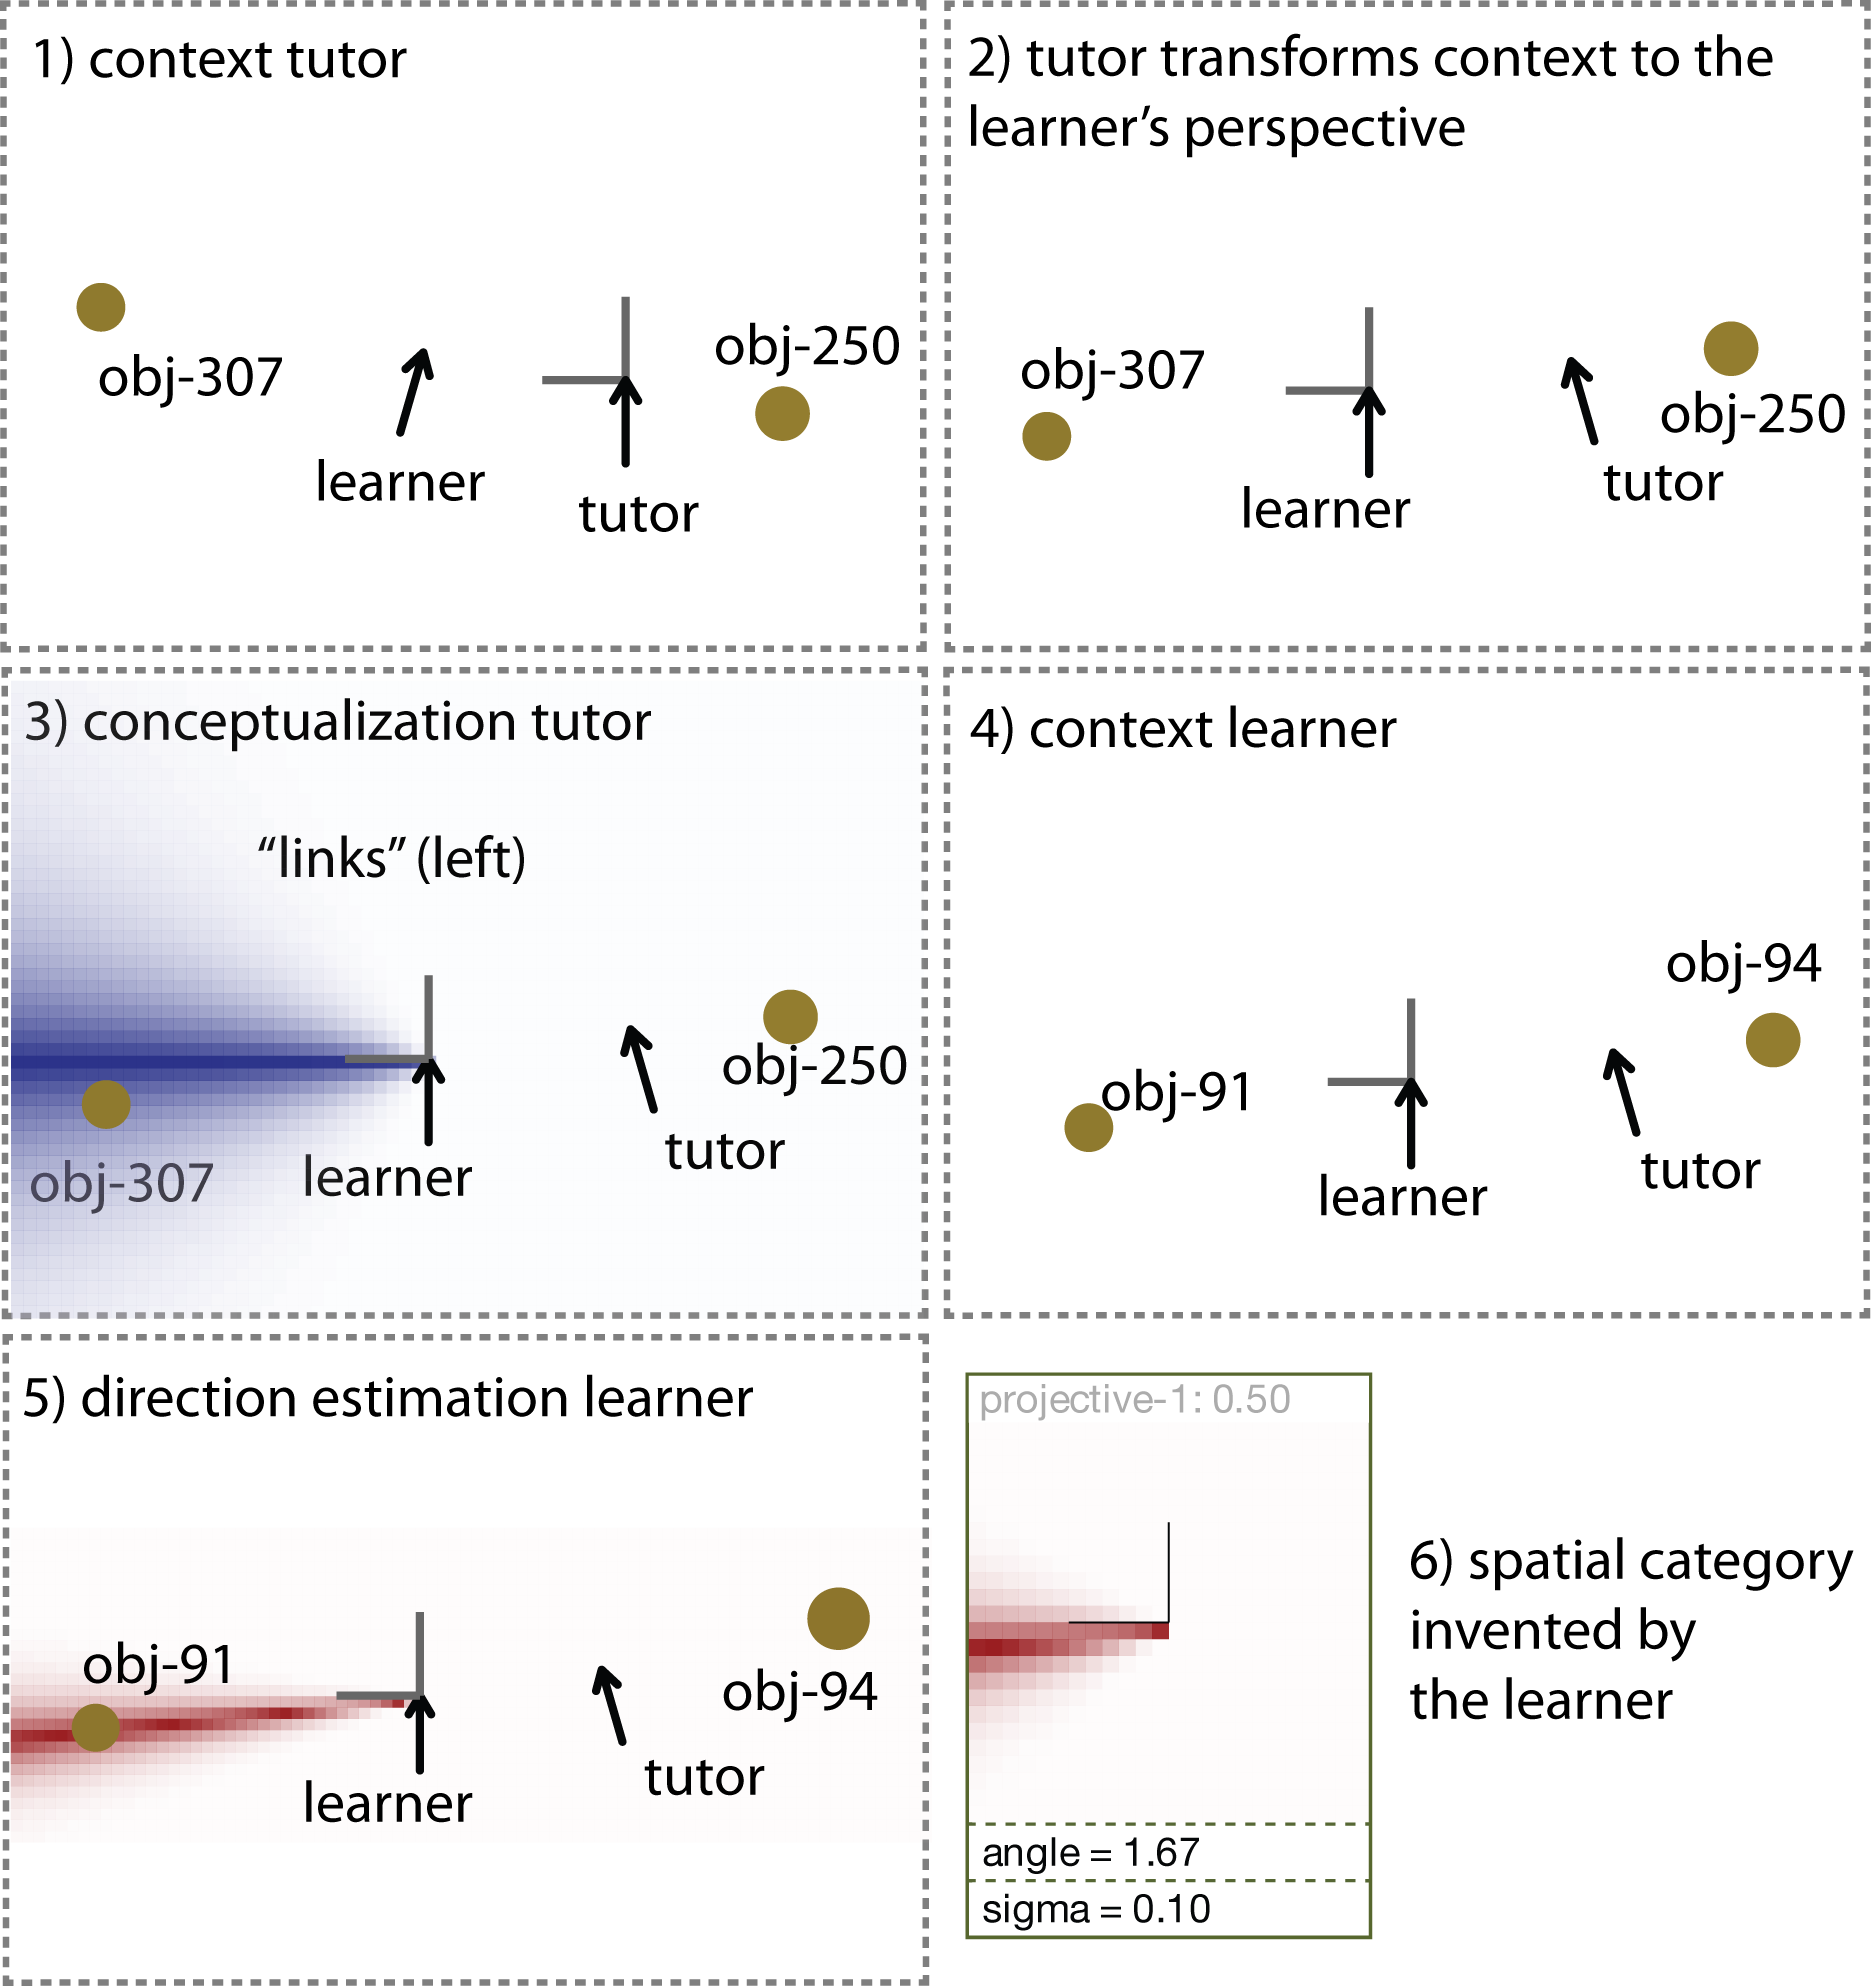
\includegraphics[width=0.75\columnwidth]{figs/category-acquisition-projective-single-category-acquisition.png}
\end{center}
\caption[Adoption of an unknown string]{This figure details the adoption of an unknown string by a learner agent in
interaction with a tutor agent. The tutor who is the speaker starts by conceptualizing for 
the topic object in his context (image~1). Here, {\footnotesize\tt obj-307} ({\footnotesize\tt obj-91} in the 
learner's context) is chosen as topic. In order to help the learner, the tutor conceptualizes 
a meaning for the topic from the perspective of the learner (image 2). For this
particular topic and context the tutor finds the category {\footnotesize\tt left}
associated with the word \textit{links} (`left') to be most discriminating (image 3). The speaker then
utters the word to the learner, who himself has a particular view of the world (image 4).
When this is the first interaction ever involving the word \textit{links}, the learner does not know
the word and the interaction fails. However, after the speaker pointed to the topic, the
hearer can adopt the string and connect it to the newly invented projective category
{\footnotesize\tt projective-1}, which derives its angle value from the direction of the topic object (image 5). 
The initial $\sigma$ is set to $0.1$. This is a low value that focusses the 
category around the direction of the topic object (image 6).}
\label{f:category-acquisition-projective-single-acquisition}
\end{figure}

\begin{figure}
\begin{center}
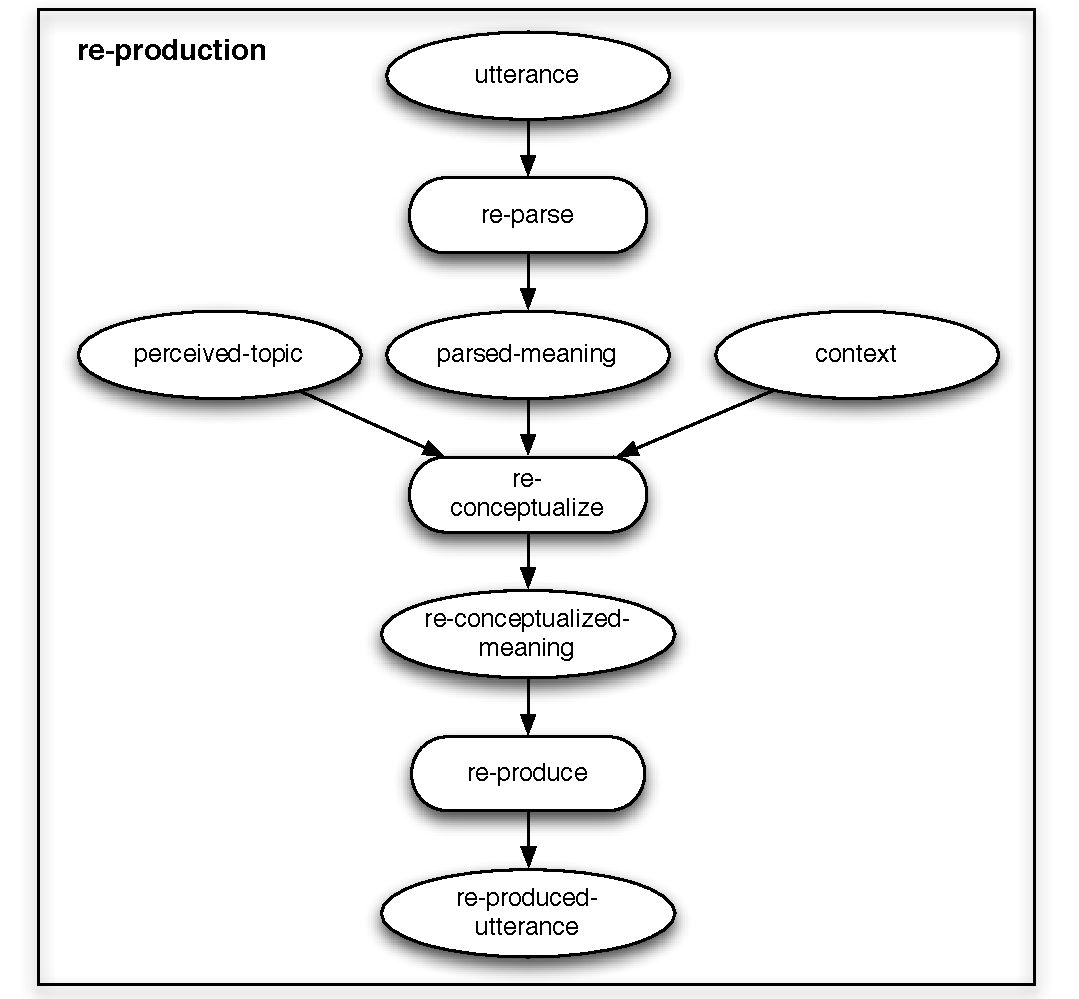
\includegraphics[width=0.75\columnwidth]{figs/task-re-production}
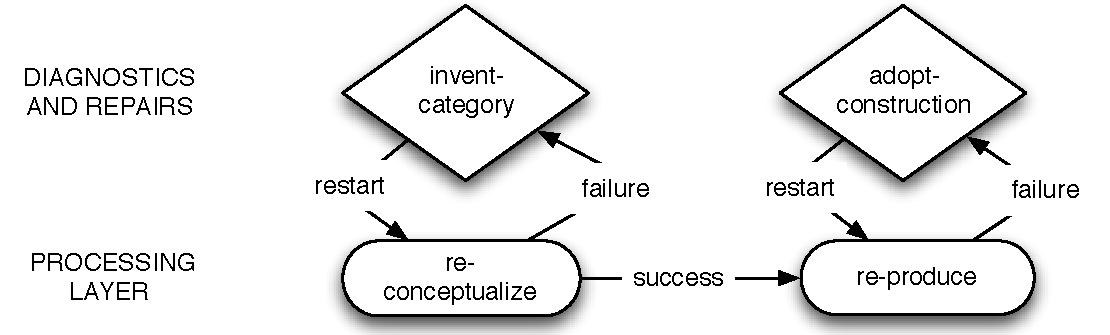
\includegraphics[width=0.75\columnwidth]{figs/diagnostics+repairs-adoption}
\end{center}
\caption[Re-production]{The top figure shows the processes that the hearer runs 
in {re-production} once it is clear that the interaction failed and 
the speaker pointed to the object ({\footnotesize\tt perceived-topic}). 
The agent {re-parses} the utterance and {re-conceptualizes} based on 
the {\footnotesize\tt perceived-topic}, the {\footnotesize\tt parsed-meaning} and the {\footnotesize\tt context}. 
{\footnotesize\tt Re-conceptualize} is similar to both {\footnotesize\tt conceptualize} (production) 
and {\footnotesize\tt find-topic} (interpretation). It uses IRL to find 
semantic structure that is compatible with the semantic structure
observed in the utterance and the topic. If 
{\footnotesize\tt re-conceptualize} is unable to find a category distinction 
for discriminating the topic, this
triggers the {\footnotesize\tt invent-category} repair strategy (bottom figure) 
which fixes the problem by 
inventing a new category. {\footnotesize\tt Re-production} continues by 
producing an utterance for the meaning ({\footnotesize\tt re-produce}). 
If the meaning includes a new category this fails 
which triggers the {\footnotesize\tt adopt-construction} repair.}
\label{f:re-production+diagnostics+repairs}
\end{figure}

% part one category invention and word adoption example
Let us suppose the tutor agent is equipped with the German projective 
lexical system and uttered the word \textit{links} (`left') in context {\footnotesize\tt scene-3398065133} 
(see Figure \ref{f:category-acquisition-projective-single-acquisition} 
to follow this example). Furthermore, let us suppose
the hearer, a student, has no knowledge of this word and, consequently, the interpretation
process fails. The hearer then waits for the speaker to point to the topic.
Upon observing the speaker point to the topic, the hearer \emph{re-produces}
for the now known topic. \textsc{Re-production} is a process by which agents try to fill 
in missing information in order to learn from the pieces of information available to them. 
Most importantly, the hearer \emph{re-conceptualizes}
a meaning for the topic, mirroring the speaker (see Figure \ref{f:re-production+diagnostics+repairs}). 
Because the agent does not yet have any spatial categories, re-conceptualize fails and 
no meaning is computed. To solve this problem the hearer invents a new category. 
The new category is directly based on the topic object. For projective categories, 
the direction vector of the new category is directly 
established from the direction the topic object lies in. When the hearer has invented 
the category he can conceptualize a meaning for the topic object and, subsequently, when trying to 
express it for himself in {re-production}, he fails, because this category is new
and he has no construction covering it. At this moment, another
repair strategy uses the conceptualized meaning and in particular the conceptualized
category, as well as the fact that there was an unparsed string to create a new 
construction that links the category with the unparsed string 
(see Figure \ref{f:category-acquisition-projective-single-acquisition-cxn} for
the new construction). After these two repairs operated, 
the learner ends up with one new category linked via the new construction to the 
word \textit{links} (`left'). The new category is based on a single example of what 
the tutor agent equipped with the German projective system would call \textit{links} (`left').

\begin{figure}
\begin{center}
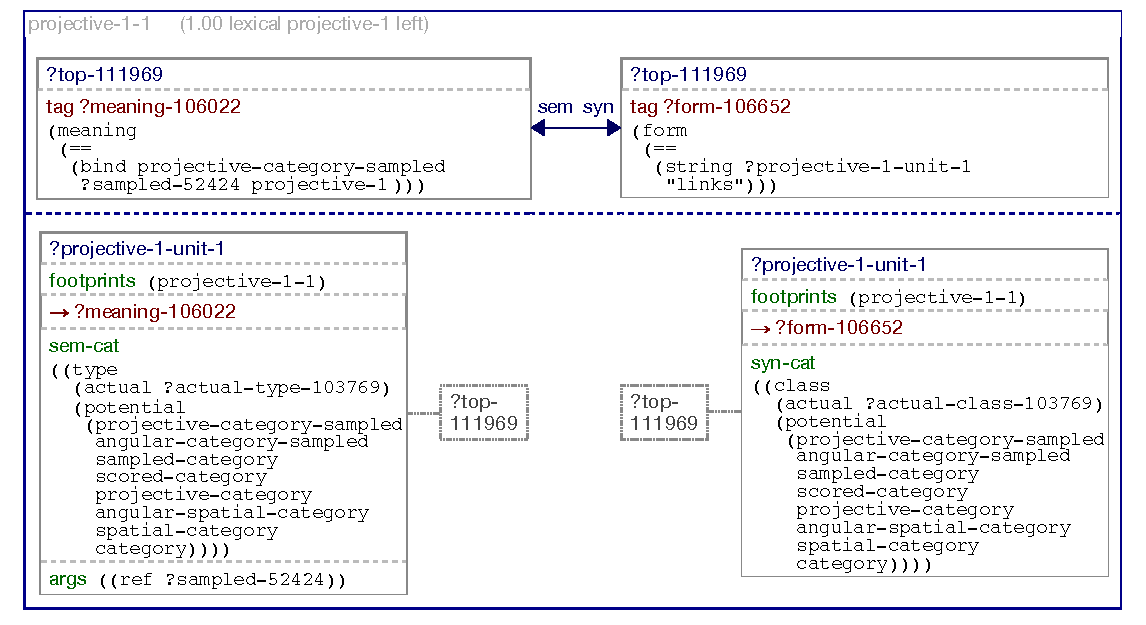
\includegraphics[width=1\columnwidth]{figs/category-acquisition-projective-adopted-cxn-left}
\end{center}
\caption[Construction invented by the repair {\footnotesize\tt adopt-construction}]{Construction invented by the repair {\footnotesize\tt adopt-construction} 
which links the string \textit{links} to the new category {\footnotesize\tt projective-1}.}
\label{f:category-acquisition-projective-single-acquisition-cxn}
\end{figure}


% general introduction alignment
Adoption is necessarily based on a single example. Consequently, the category
adopted by the hearer might be quite different or at least dissimilar to the category
that the tutor used. Learners need a mechanisms that align the category 
representation of over many interactions with that of the target language system. 
Of course, the learner can never directly read out 
the category the tutor uses in communication, hence, the only possible source of 
data for learners are the samples of objects that the tutor names using the same word, 
that is to say, the topic objects in interactions in which one of the agents actually uses 
the concept associated with a particular string, for example, the word {\itshape links} (`left'). Category representations are updated in a continuous manner 
from interaction to interaction by adding samples and re-estimating the components of 
the representation. For projective categories, samples are used to 
re-estimate the prototypical direction by computing the mean direction vector of 
the samples using the following formula for averaging the angles of the samples $S$.
\begin{equation}
a_c = 
%\operatorname{atan2}
\left(\frac{1}{|S|}\sum_{s\in S}\sin a_s,\frac{1}{|S|}\sum_{s\in S}\cos a_s\right)
\label{e:update-a}
\end{equation} 
On top of that, the new $\sigma$ value $\sigma'$ 
which governs the shape of the similarity function is adapted using the following formula.
\begin{equation}
\sigma'_c = \sigma_c + \alpha_\sigma \cdot \left(\sigma_c - \sqrt{\frac{1}{|S|-1}\sum_{s\in S}(a_c - a_s)^2}\right)
\label{e:update-sigma-a}
\end{equation} 
This formula describes how much the new $\sigma_c$ of the category $c$ 
is pushed in the direction of the angle standard deviation of the sample set 
by a factor of $\alpha_\sigma \in [0,\infty]$. Naturally, alignment and
adoption operators have quite a number of parameters, for instance
how many samples to consider, how eager to update the $\sigma$ component using
$\alpha_\sigma$ and so on and so forth. These parameters are typically quite robust and little to
medium changes do not affect the overall performance of the system.

\is{alignment}
Alignment is not only important for re-estimating the category representation,
but it also extends to all levels of semantic and syntactic processing. Every item 
in the inventory of an agent including every category and construction is scored. 
After each interaction scores of these items are updated by alignment operators 
based on the usage and communicative success. 
For lexical systems, the two important components are
lexical constructions and categories. Student agents increase the score of successfully
used constructions and categories and decrease the score 
if the item was used unsuccessfully. Constructions and categories with 
a score lower than or equal to $0$ are removed from the inventory. 

% category development over time
\begin{figure}
\begin{center}
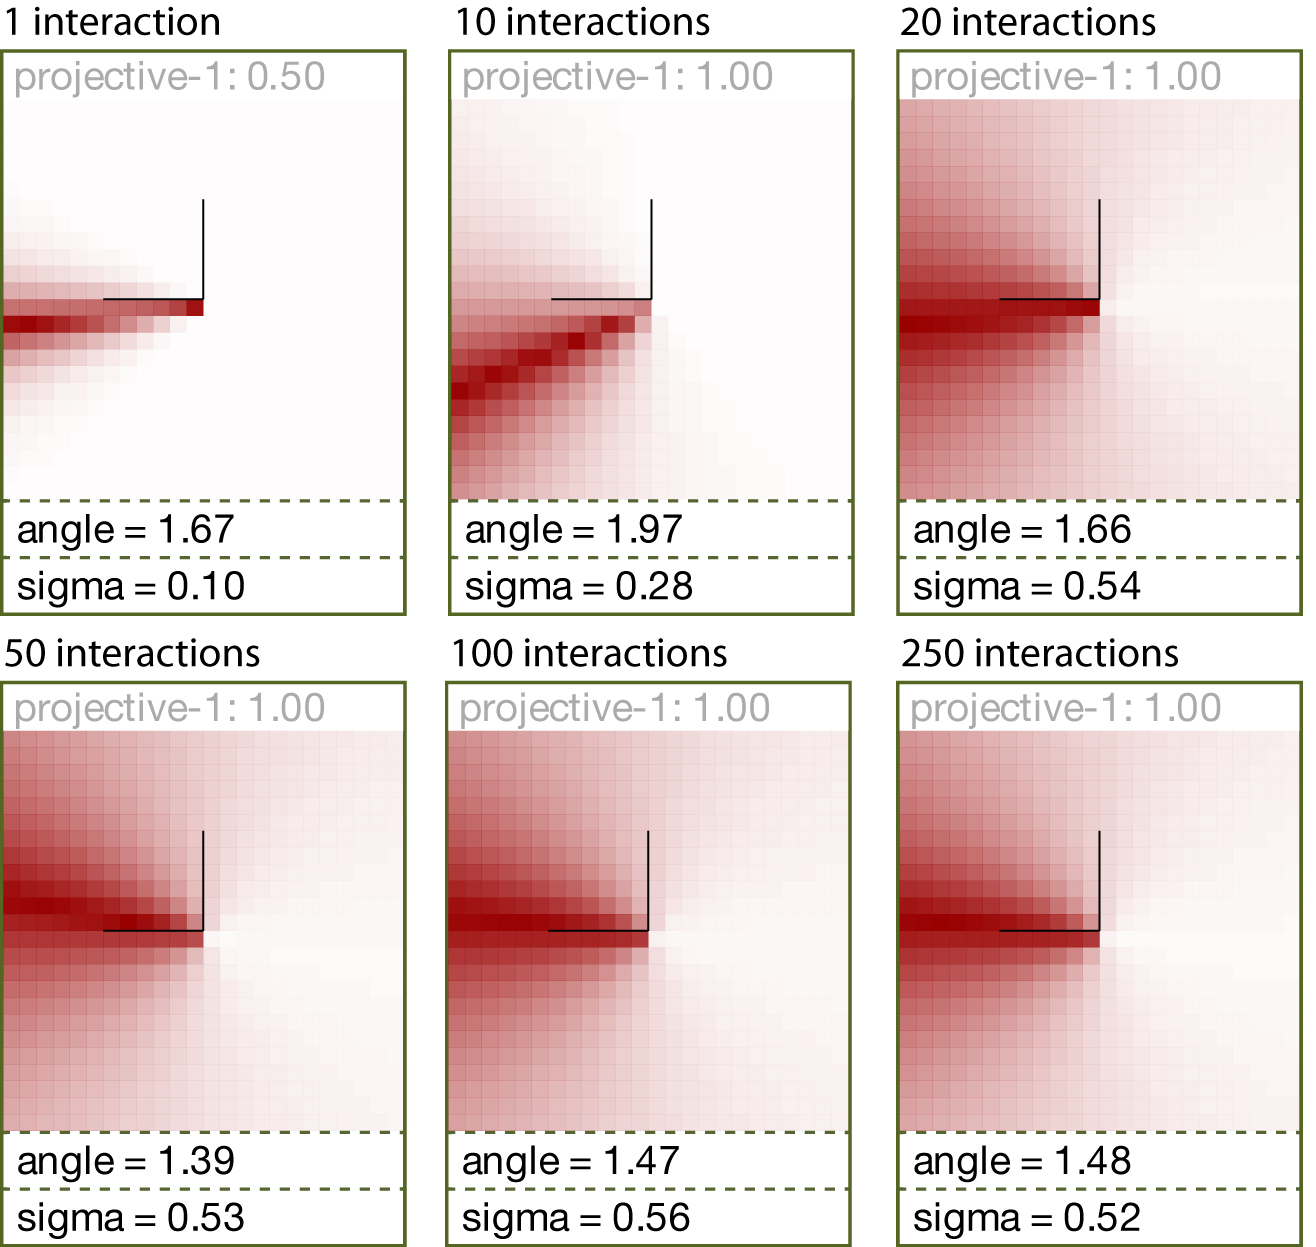
\includegraphics[width=0.8\columnwidth]{figs/category-acquisition-projective-category-development-over-time.png}
\end{center}
\caption[Development of a projective category]{Development of the projective category whose initial adoption is depicted in 
Figure \ref{f:category-acquisition-projective-single-acquisition} over many interactions 
(after 1, 20, 50, 100 and 200 interactions). In the beginning the width of the category is narrow (small $\sigma$). Gradually 
its direction approaches the direction of the target category {\footnotesize\tt left} and so does its $\sigma$ 
(the target category's $\sigma$ is $0.4$).}
\label{f:category-acquisition-projective-development-over-time}
\end{figure}

\subsection{Experimental setup and measures}
One can test the performance of the learning operators discussed above and their 
sufficiency for acquiring a language system by applying them in populations
of two agents. One of the agents, the tutor agent, is equipped with a fully 
developed projective category system and corresponding lexical items. 
The second agent, the learner agent is equipped with the learning operators.
Both agents are situated in the real world and are given the task to talk about
objects in their environment in a spatial language game. The population
continuously interacts over a number of interactions. Success, performance
and development of the population are tracked with a variety of measures.
\begin{description}
\item[Communicative Success] \is{measures!communicative success}Communicative success is the most important
measure as it reflects the overall performance of the population. Every interaction
is either a success or a failure. Success is counted as $1.0$ and failure 
is counted as $0.0$. 
\item[Number of Categories per Student] \is{measures!number of categories}This measure counts 
the number of categories known to student agents. 
Besides number of categories, number of constructions\is{measures!number of constructions} is an often
used measure in acquisition experiments.
But, since the number of categories is equal to the number of constructions, 
measuring the number of constructions\is{measures!number of constructions} is omitted for the acquisition experiments
\item[Interpretation Similarity] \is{measures!interpretation similarity}This measure tracks how similar the 
interpretation of each word known to the tutor is to that of the student. 
Technically this is measured by comparing the category the tutor links
to a specific word to the category the student links to the same word.
Since projective categories are described by a direction and a similarity function 
width parameter $\sigma$, two categories are most similar when both angle 
and $\sigma$ are equal. The precise formula is based on the repertoire of 
words $W(a_{tut})$ known to the tutor 
$a_{tut}$ and the similarity of the category $C(a_{tut},w)$ the tutor 
associates with each word $w$ to the category the learner $a_{learn}$
associates with that word $C(a_{learn},w)$
\begin{equation*}
\operatorname{I} (a_{tut},a_{learn}) 
= 
\frac{1}{|W(a_{tut})|}\sum_{w \in W(a_{tut})} 
\operatorname{s} \left(C(a_{learn},w),C(a_{tut},w)\right)
\end{equation*}
If the learner has no category associated with a particular word $w$, i.e., when $C(a_{tut},w)$ 
does not find a category, the similarity is $0$. If, however, the learner has some projective category
associated with the word, then $\operatorname{s}$ is defined as follows.
\begin{equation*}
\operatorname{s}(c,c')=e^{-\frac{1}{2}(a_c - a_c')^2\frac{2}{\sigma_c + \sigma_c'}}
\end{equation*}
\end{description}

To be sure that this approach to acquisition works reliably, acquisition is not only tested
in a single population, but multiple experiments are run in which learners have to 
acquire the lexical systems of the tutors. In every interaction between a tutor and a learner certain 
choices are random. Which agent is speaker? Which agent is hearer? Which object is topic? 
These are all choices that are made using a random number generator. Particular
choices may or may not favor the acquisition of the lexical system by the learner. 
To account for such effects, 25 experiments are run in parallel, each starting with a 
student which initially knows no categories, no words and no constructions linking them. 
The progress of each such run is measured simultaneously, and, finally, all results are 
collected and the measures are averaged over the 25 runs.

\begin{figure} 
\begin{center}
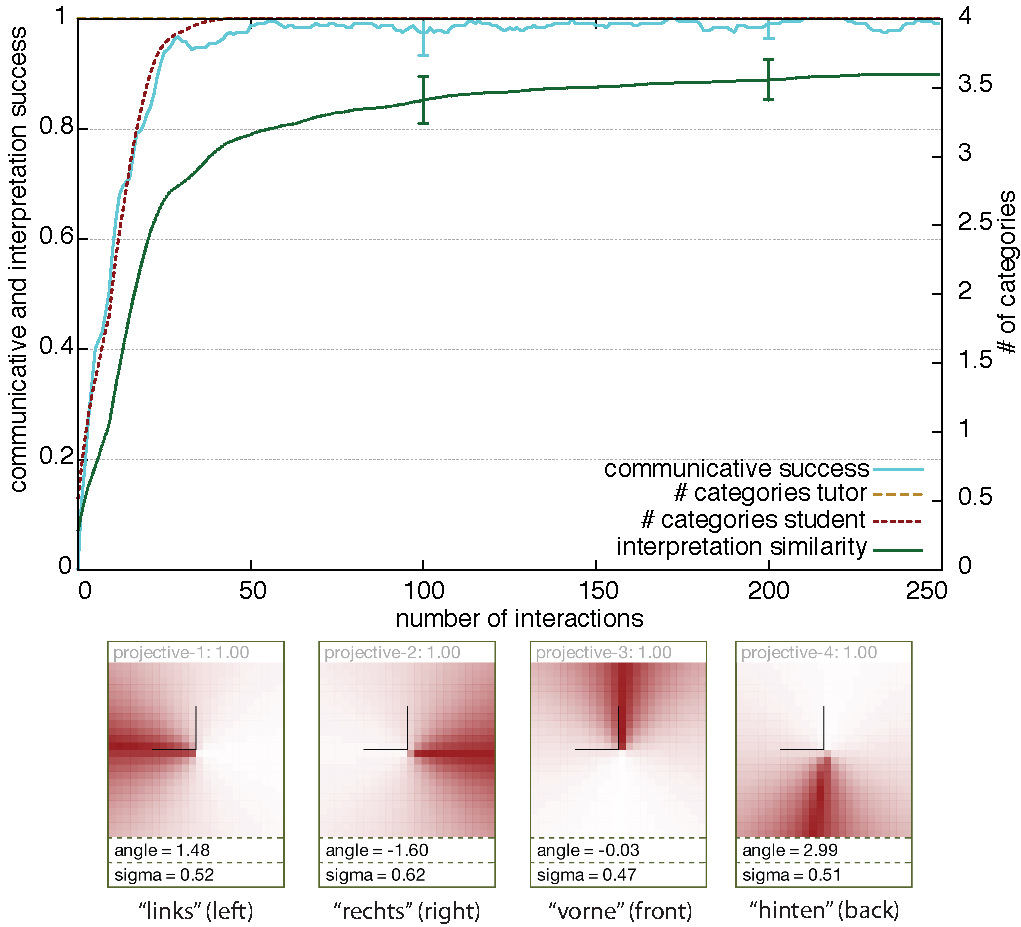
\includegraphics[width=0.8\columnwidth]{figs/category-acquisition-projective-results+categories}
\end{center}
\caption[Results acquisition of the projective system]{%
The top figure shows the dynamics of 
acquisition experiments over many interactions (25 runs averaged) in which 
a learner is trying to acquire the projective language system from a tutor.
Agents quickly reach communicative success (the base line experiment of tutors communicating 
reaches ~98\% success for the same data set). After roughly 25 interactions, all categories and their 
corresponding strings have been adopted (the number of categories approaches 4)\is{measures!number of categories}. 
In the remaining interactions the alignment operator drives the {interpretation
similarity} towards 1.0 (which is the highest value and signifies total overlap between the categories
of the tutor and the learner). Interestingly, communicative success\is{measures!communicative success} correlates
with the number of categories\is{measures!number of categories} of the student more than it does with interpretation similarity.\is{measures!interpretation similarity}
This shows that agents do not need perfectly aligned categories to be able to communicate successfully.
The bottom figure shows the categories acquired by a learner in one 
particular population of an acquisition experiment and to which strings they are linked. 
The resulting categories are very similar to the projective categories given to the tutor.}
\label{f:category-acquisition-projective-results}
\end{figure}

\subsection{Results}
Interestingly enough, the basic mechanisms for adoption and alignment
are sufficient to get a learner agent to acquire the German projective category 
system from a tutor. Figure \ref{f:category-acquisition-projective-results}
shows the results of 25 populations each consisting of one tutor and one student
averaged over 250 successive interactions. Clearly, the learner agent is able to increase
its communicative ability while adopting the lexical system of the tutor agent,
which manifests in the increase in average communicative success\is{measures!communicative success}
over interactions which progressively approaches the value of $1$. Two tutors 
interacting on the same data set interact successfully in 98\% of the cases, which
makes for a \emph{baseline} communicative success of $1.0$. So we can conclude that
the learner easily acquires similar communicative abilities.
These positive developments are on the one hand a result of
successful adoption of words and categories, but on the other hand, they are due to
the alignment operators that gradually push the categories of the learner agent 
to become more and more similar with those of the tutor which can be seen with 
the increase in interpretation similarity. Lastly, one can check the number of categories\is{measures!number of categories} acquired
which gradually approaches the number of categories\is{measures!number of categories} in the target language system.

\begin{figure}
\begin{center}
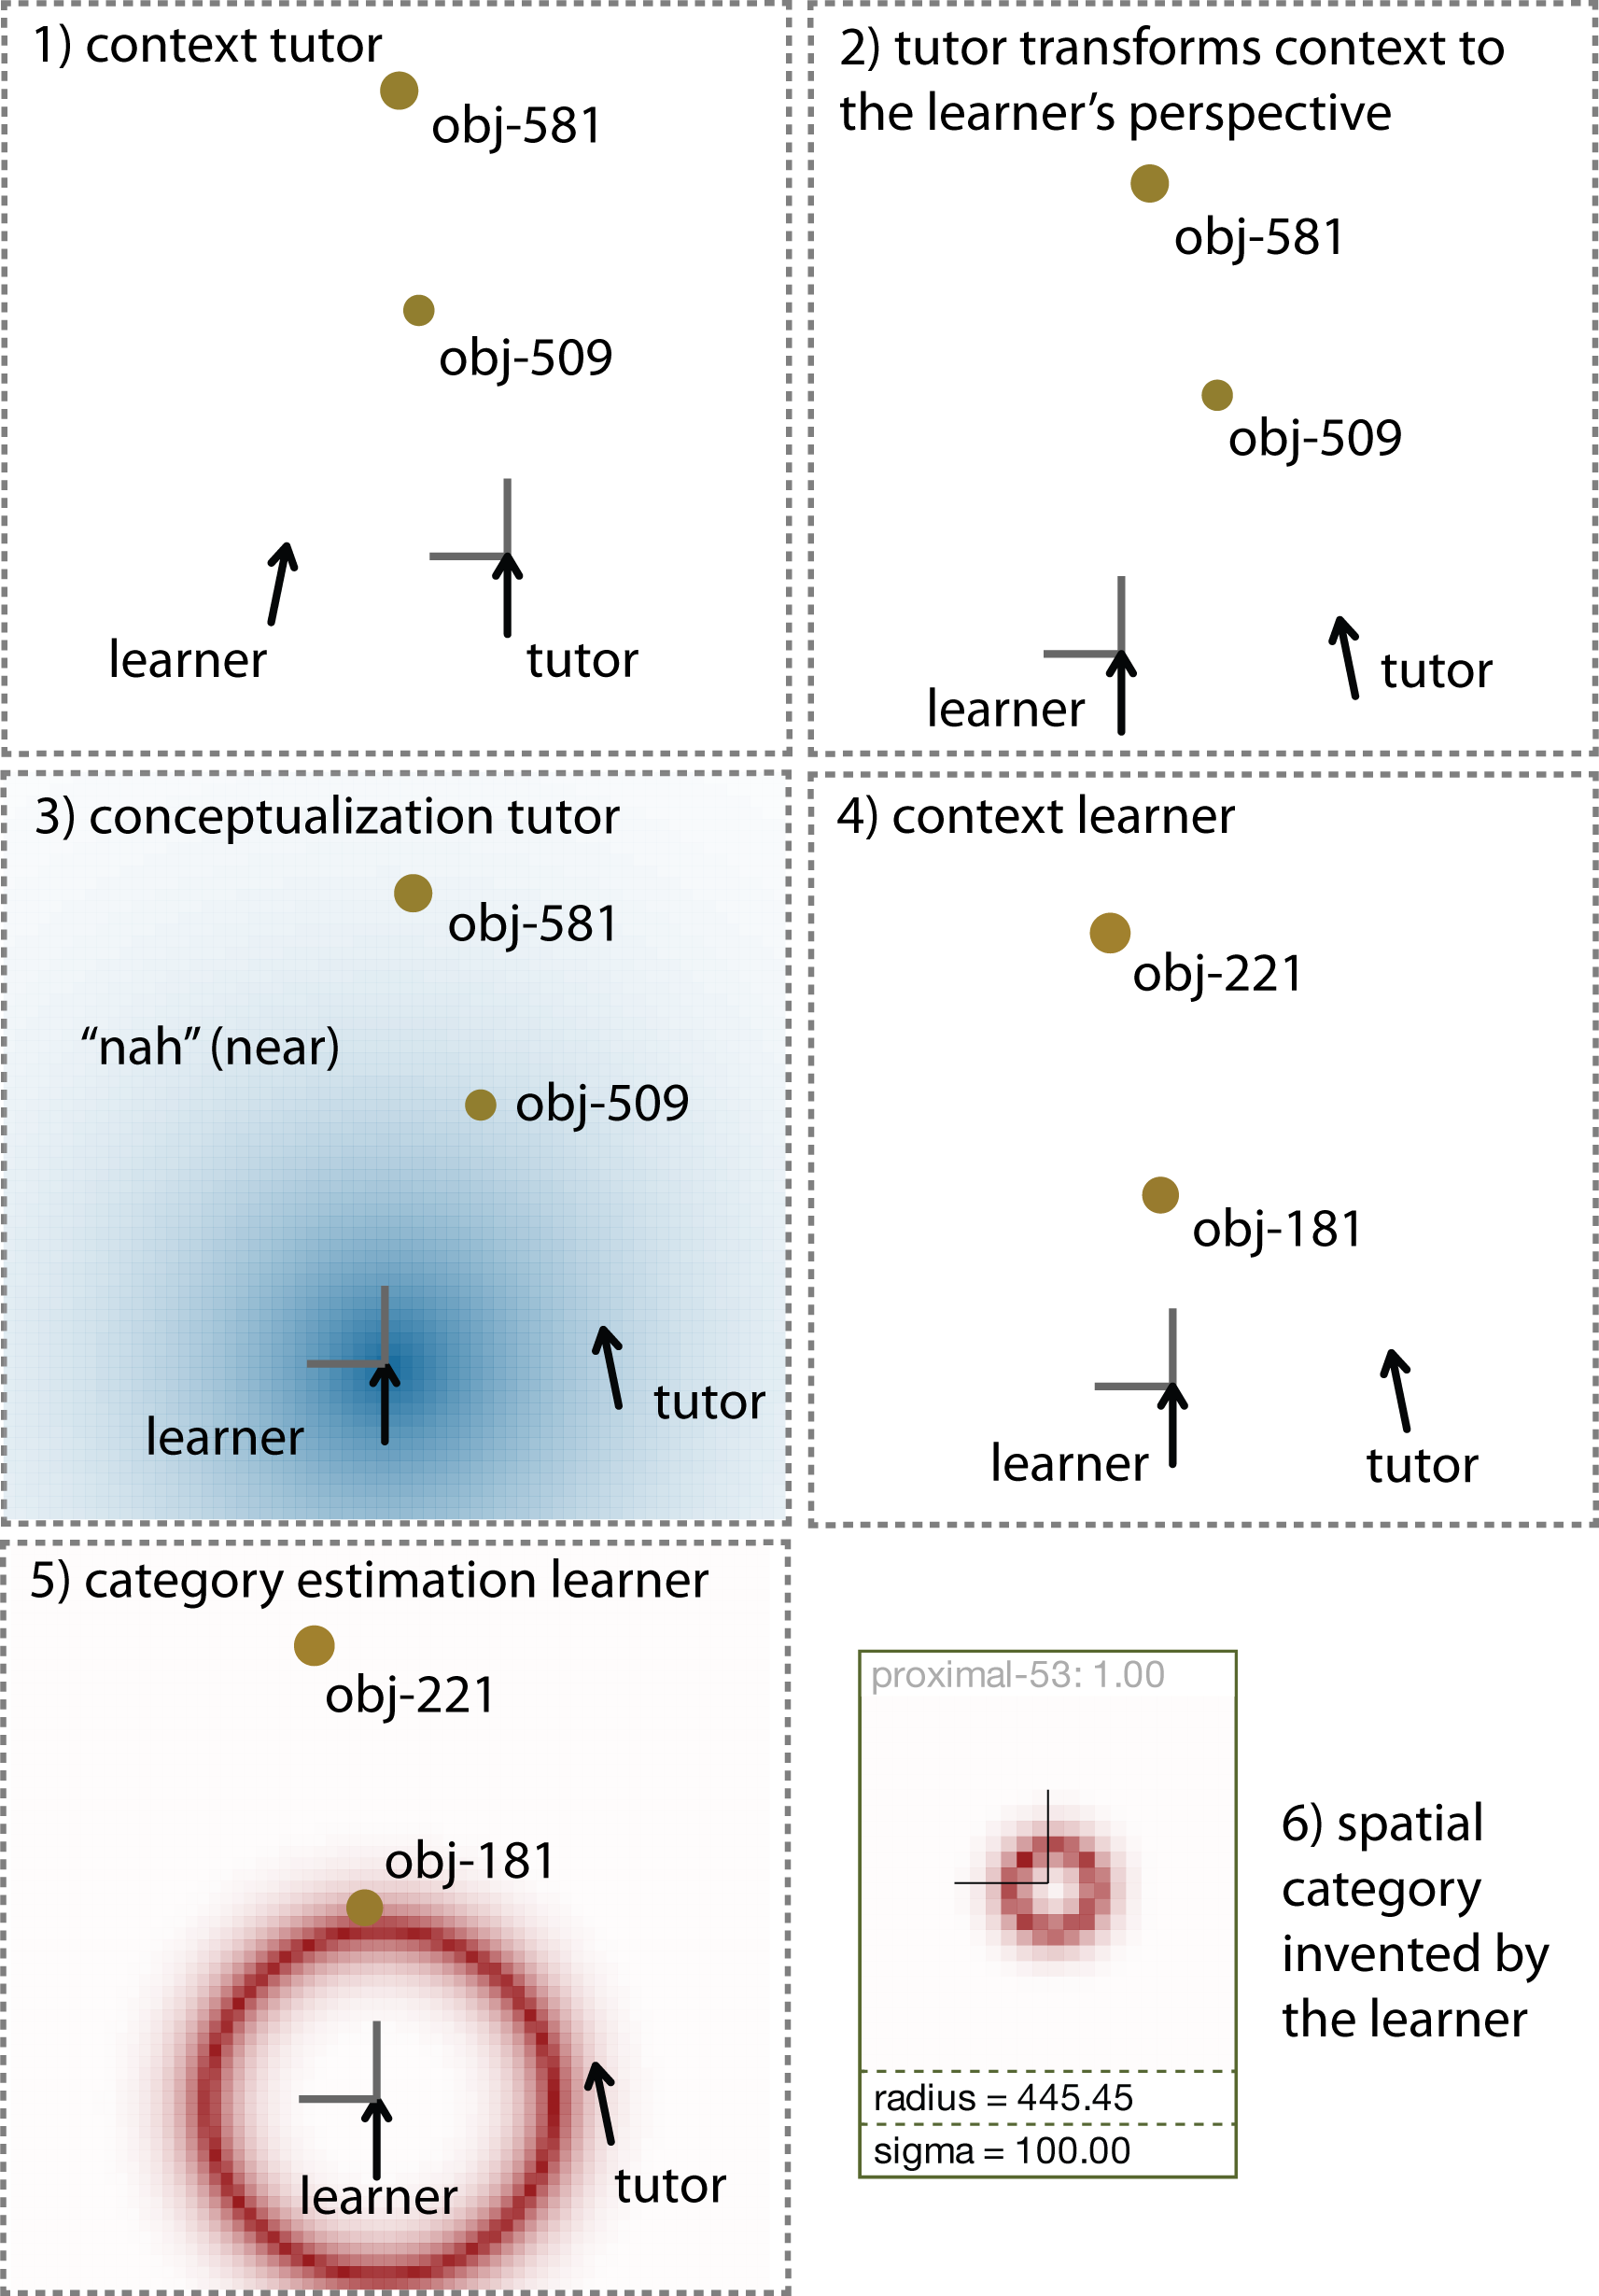
\includegraphics[width=0.8\columnwidth]{figs/category-acquisition-proximal-single-category-acquisition.png}
\end{center}
\caption[Acquisition of a single proximal category]{Acquisition of a single proximal category. The sequence of steps 
are the same as for projective categories. However, since the the tutor is equipped with
proximal categories, he conceptualizes a proximal category for the topic object ({\footnotesize\tt obj-181} 
in his context). In contrast to the projective case, the learner uses the distance of the 
topic object ({\footnotesize\tt obj-181} in his context) to build the new category.}
\label{f:category-acquisition-proximal-single-acquisition}
\end{figure}

% example for proximal concrete strategy 
\subsubsection{Acquisition of the proximal system}
Similar learning operators are sufficient for learners to acquire the 
German proximal spatial category system. The only difference is 
that the learning operators are adapted to proximal categories. So, for instance,
instead of using the direction of the topic object as a seed for a new category,
its distance is used (Figure \ref{f:category-acquisition-proximal-single-acquisition} 
details the process). Consequently, the alignment operators are also 
adjusted to use the average distances of samples and to 
update the $\sigma$ of the categories using distances of sample objects. 
\begin{equation}
d_c = \frac{1}{|S|}\sum_{s\in S} d_s
\label{e:update-d}
\end{equation} 
\begin{equation}
\sigma'_c = \sigma_c + \alpha_\sigma \cdot \left(\sigma_c - \sqrt{\frac{1}{|S|-1}\sum_{s\in S}(d_c - d_s)^2}\right)
\label{e:update-sigma-d}
\end{equation} 
Furthermore, the adoption operator for constructions linking an invented proximal category to 
an observed string is the same as for projective category acquisition.
We can test the performance of the learning 
operators using a population of agents where one agent, the tutor, 
is equipped with the German proximal system, and the other agent, 
the learner, starts without any knowledge 
of the system and is given proximal category adoption and alignment
operators to acquire the system from the tutor. Figure \ref{f:category-acquisition-proximal-results}
details results for proximal categories. The graph shows that 
the acquisition and alignment operators enable the learner to quickly pick up the
two projective categories. Interpretation similarity also quickly rises; however,
it stays low and does not approach $1.0$ as in the case of projective categories. 
If one looks at the resulting categories of one particular run 
(bottom Figure \ref{f:category-acquisition-proximal-results}), 
one can easily see the reason for this. First, both the distance prototype of the proximal category 
associated to the word \textit{nahe} (`near') as well as the distance prototype associated with the word 
\textit{fern} (`far') do not have the same values as the corresponding tutor categories, which have been
setup with $0.0$ for near and $2000.0$ for far. Second, the $\sigma$ values for these categories also
do not overlap sufficiently ($\sigma$ values in tutor categories are equal to $1000.0$). 
The reason for this is the distribution of objects in the spatial scenes used in the experiments. 
No object is ever further away than about $1500.0$ mm and no object is so close to any of the robots as to approach
a distance of $0.0$. So the alignment operator has no chance of picking up values even close
to the ones set in the tutor categories. The categories acquired by the learner, in other words,
accurately reflect the actual distribution of objects in the spatial scenes rather than the 
values picked for the tutor. Nevertheless, learner and tutor are capable of 
communicating successfully after the system stabilizes.


\begin{figure} 
\begin{center}
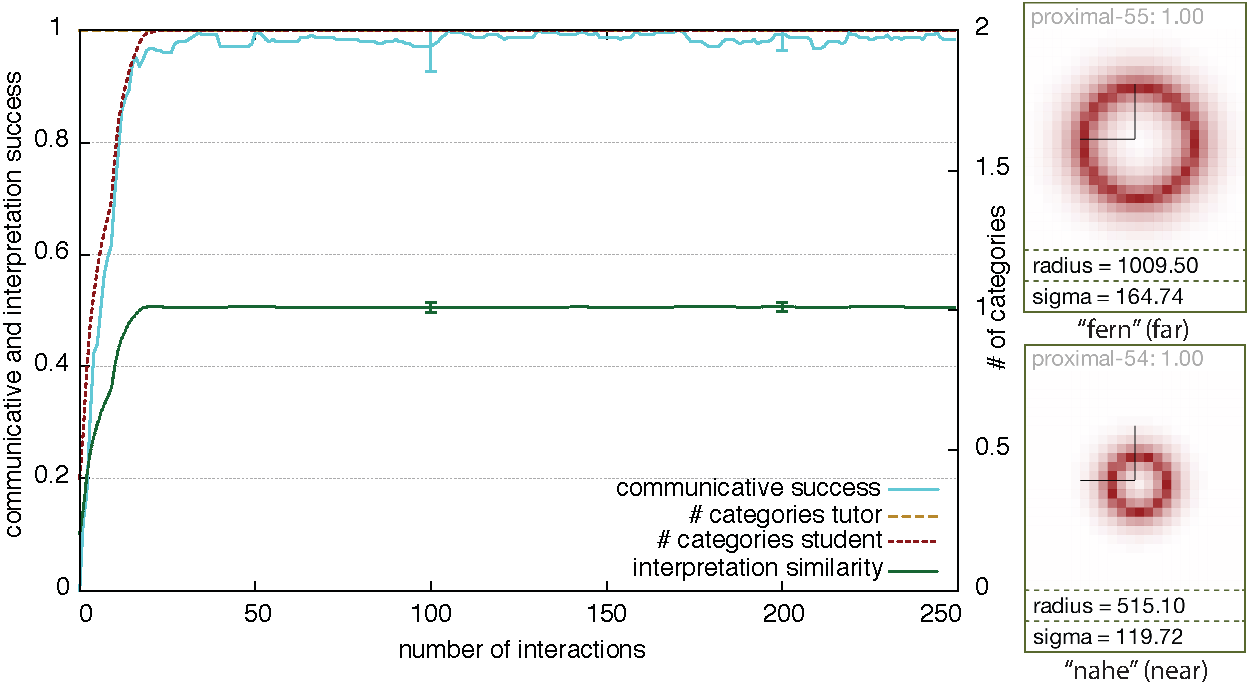
\includegraphics[width=1.0\columnwidth]{figs/category-acquisition-proximal-results+categories}
\end{center}
\caption[Results acquisition of the proximal system]{This figure shows the dynamics of acquisition experiments over many interactions (25 runs averaged, 
left image) in which the tutor possess a proximal language system. 
Agents quickly reach communicative success\is{measures!communicative success} (the base-line experiment of tutors communicating 
reaches 98\% success for the same data set). To the right, categories acquired by a learner in 
one particular run of such an acquisition experiment are shown.}
\label{f:category-acquisition-proximal-results}
\end{figure}

\begin{figure}
\begin{center}
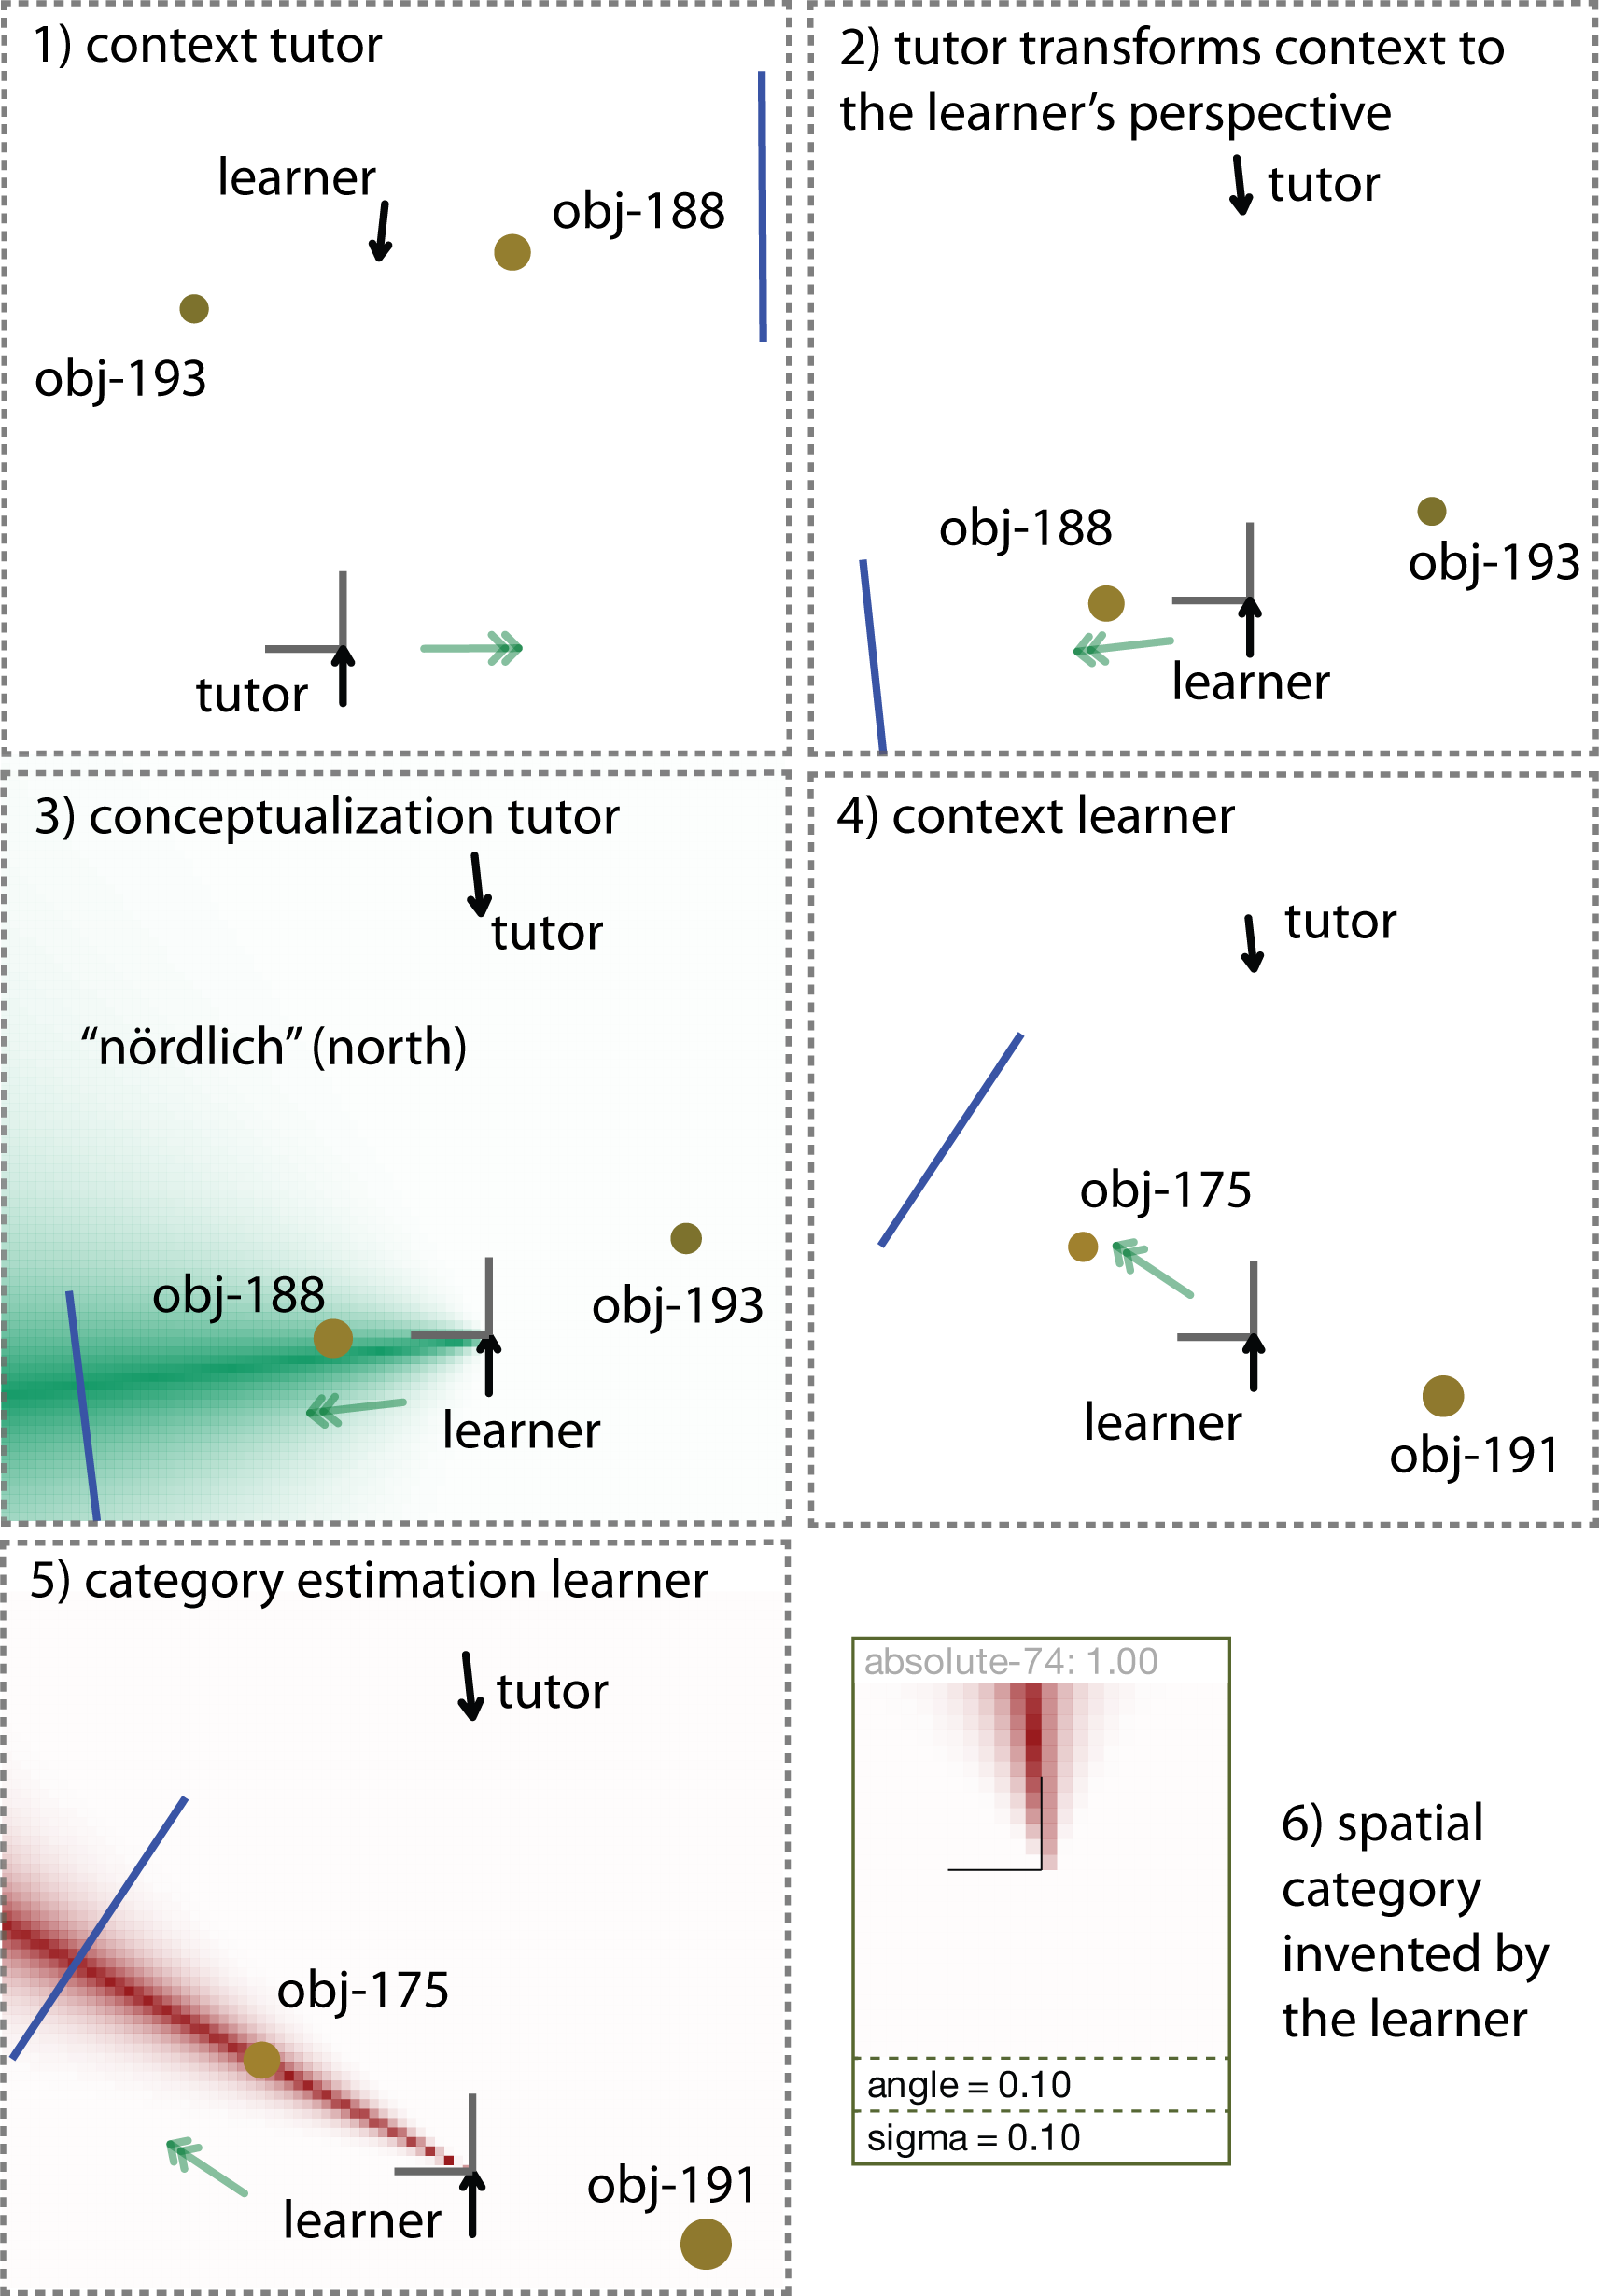
\includegraphics[width=0.8\columnwidth]{figs/category-acquisition-absolute-single-category-acquisition.png}
\end{center}
\caption[Acquisition of a single absolute category]{%
Acquisition of a single absolute category. The steps are the 
same as for projective and proximal categories, but the tutor 
conceptualizes using absolute categories which
implies that he needs to take into account the direction to 
the global reference (green arrow).
Consequently, the learner uses the direction to the topic object 
(here {\footnotesize\tt obj-188} in the tutor's context and {\footnotesize\tt obj-175} in the learner's context)
given the global direction to build a new category.}
\label{f:category-acquisition-absolute-single-acquisition}
\end{figure}


\subsubsection{Acquisition of the absolute system}
The last group of categories in the German language system discussed in this book
are absolute categories like {\footnotesize\tt north} and {\footnotesize\tt east} and so forth. Again,
the learning operators are adapted to be specialized on the acquisition of absolute
categories, which are very similar to projective categories in that they focus on
the angular dimension (the same formulas apply). The only real difference to
projective categories is that absolute categories are applied slightly differently
by taking the global reference into account. Figure 
\ref{f:category-acquisition-absolute-single-acquisition} details the acquisition
of a single absolute category and results of acquisition are shown 
in Figure \ref{f:category-acquisition-absolute-results}. One can conclude that
acquisition of absolute categories is easily established using the 
learning operators suggested.

\begin{figure} 
\begin{center}
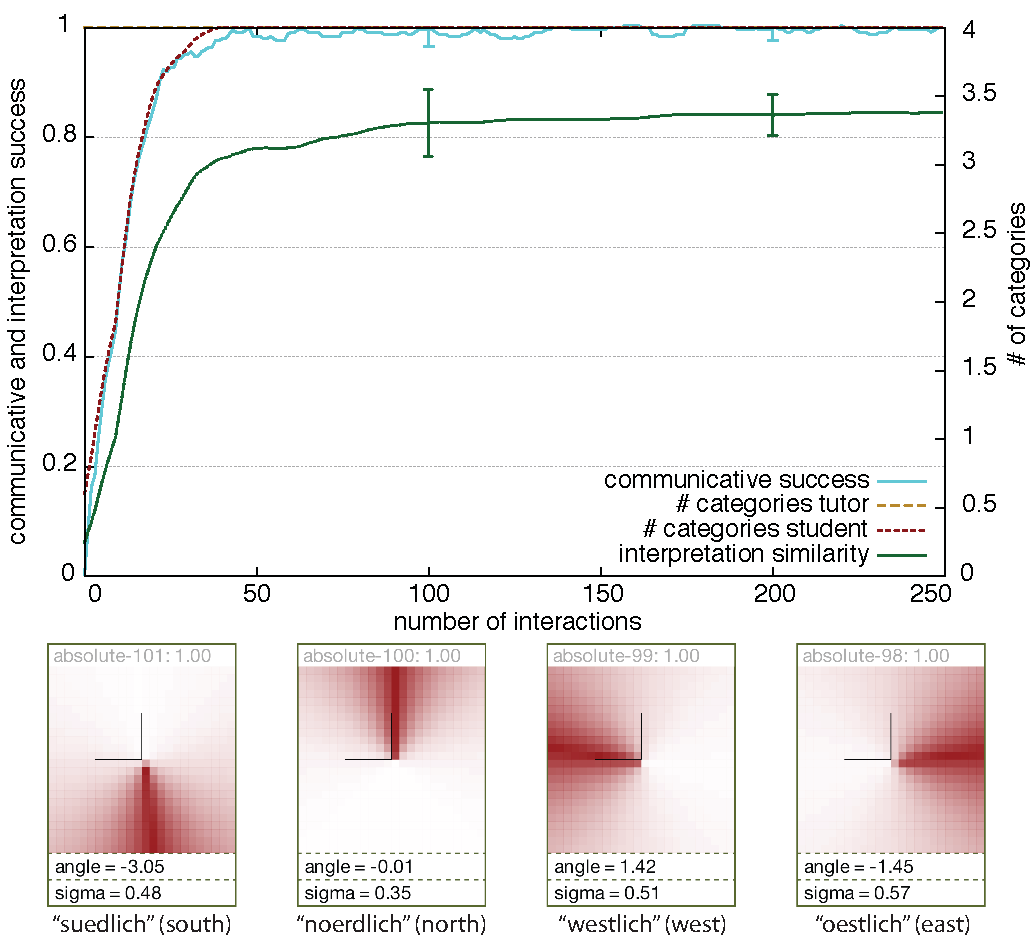
\includegraphics[width=1.0\columnwidth]{figs/category-acquisition-absolute-results+categories}
\end{center}
\caption[Results acquisition of the absolute system]{This figure shows the 
dynamics of absolute category acquisition experiments 
over many interactions (25 runs averaged, 
left image). Agents quickly reach communicative success (the base-line experiment 
of tutors communicating reaches 98\% success for the same data set). 
The bottom figures show the categories acquired by a learner in one particular run of such 
an acquisition experiment. The interpretation similarity\is{measures!interpretation similarity} develops comparably to the projective
case.}
\label{f:category-acquisition-absolute-results}
\end{figure}

\subsubsection{Co-acquisition of lexical systems}
In all the above experiments, learners were acquiring a single category type,
e.g., either projective, proximal or absolute. This entails that learners 
upon hearing a new term could be absolutely sure about the 
category type the speaker used for conceptualizing reality.
The problem with this approach is, of course, that this is rarely ever the
case in acquisition and the learner never knows what type of category he is 
supposed to acquire based solely on the word
he is observing. So the challenge remains as to how learners 
can acquire a complete system of spatial categories including proximal, 
projective and absolute categories at the same time. 

\begin{figure}
\begin{center}
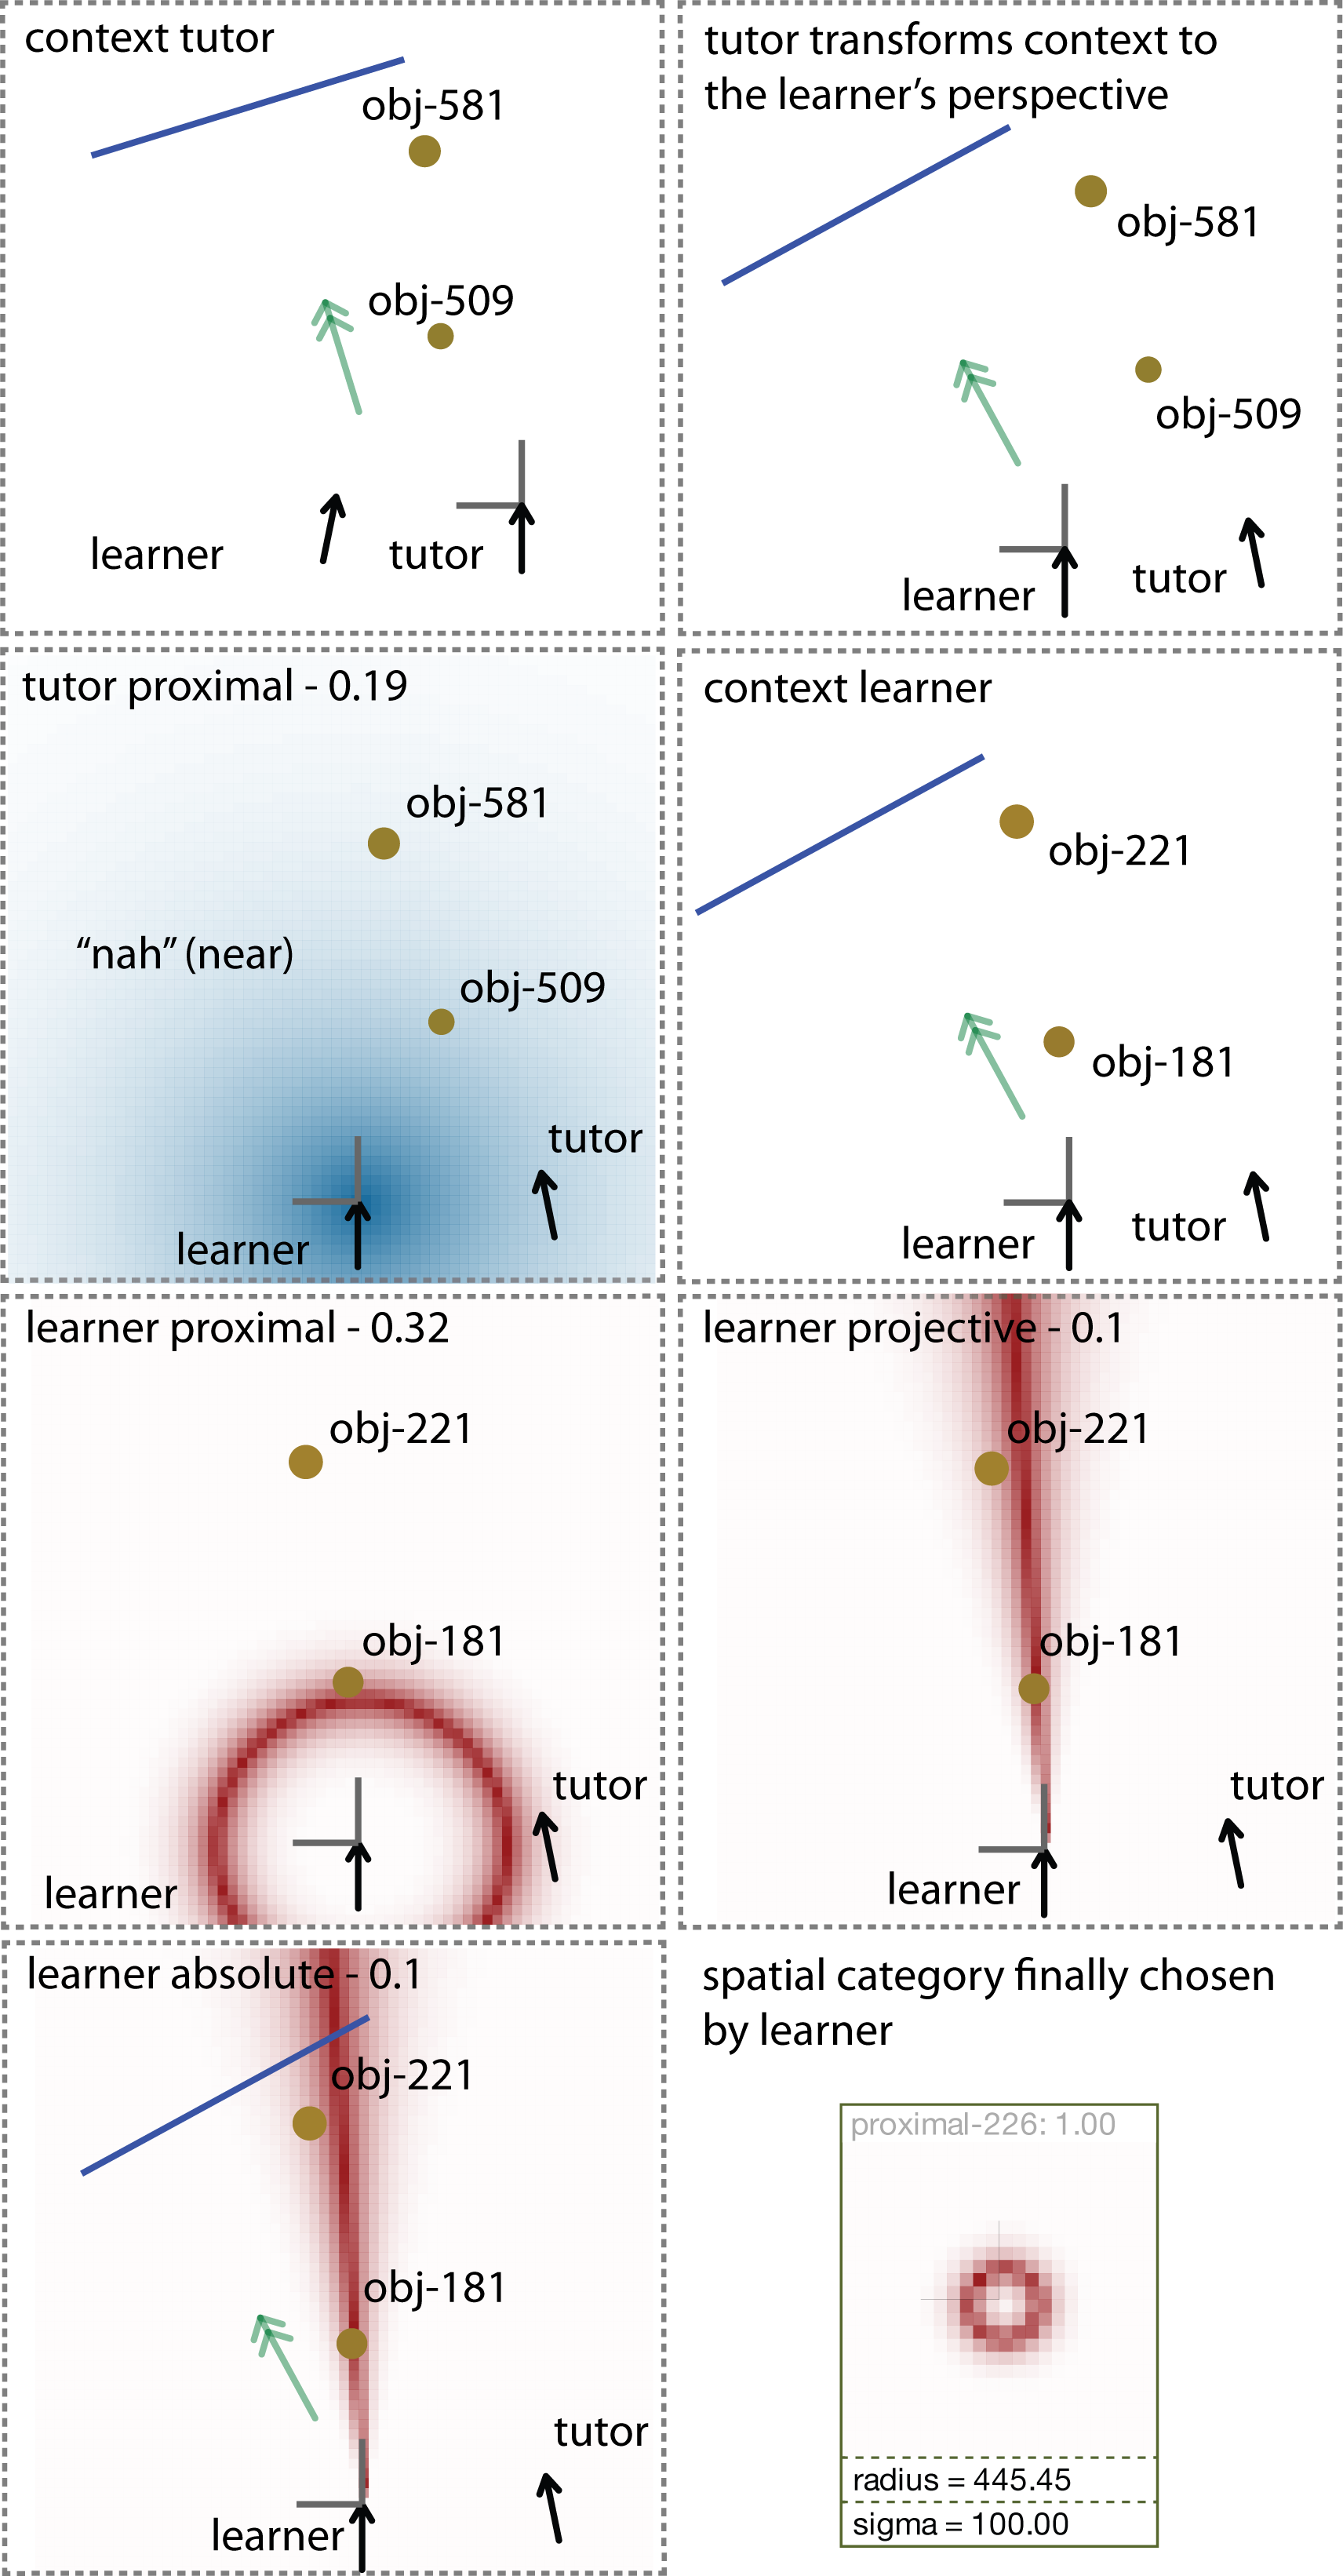
\includegraphics[width=0.7\columnwidth]{figs/category-acquisition-absolute+proximal+projective-single-category-acquisition.png}
\end{center}
\caption[Inference in re-conceptualization]{Inference in re-conceptualization}
\label{f:category-acquisition-absolute+proximal+projective-single-acquisition}
\end{figure}

% cross-situational learning? attention in thex? reference
One idea is to endow the learner with additional machinery.
What if the learner has the ability to make a best guess on 
what type of category he should learn based on discriminative power
(see \citealt{steels1997distinctions}\index{Steels, L.} for similar ideas). 
In other words, the learner should choose the particular category type
based on the current context, the topic object and, in particular, based on 
the discriminative power of each category type in the current situation.
It turns out, that we can easily use this insight to enhance the system. 
Instead of inventing a single category, the learner invents three
categories one for each category type and in re-conceptualization chooses
the category which \emph{maximizes discriminative power}.
In other words he chooses the category with the highest discrimination score. 
It is this category which survives the 
competition with the other two and it will be associated with the observed string
using a newly invented construction, while the losers will be removed.
Figure \ref{f:category-acquisition-absolute+proximal+projective-single-acquisition} 
gives an example of the process (Figure \ref{f:re-production-branching} sketches the implementation).
In the example of the figure the tutor used the projective 
category {\footnotesize\tt near} to conceptualize for the topic 
{\footnotesize\tt obj-509} (in his context). The learner invents three 
different categories one proximal, one projective and one absolute and
uses them to re-conceptualize for the topic ({\footnotesize\tt obj-175} in his context). 
The proximal category has the highest discrimination score 0.32 
and is, consequently, chosen by him as the seed for the projective 
category linked to the word \textit{nahe} (`near').

\begin{figure} 
\begin{center}
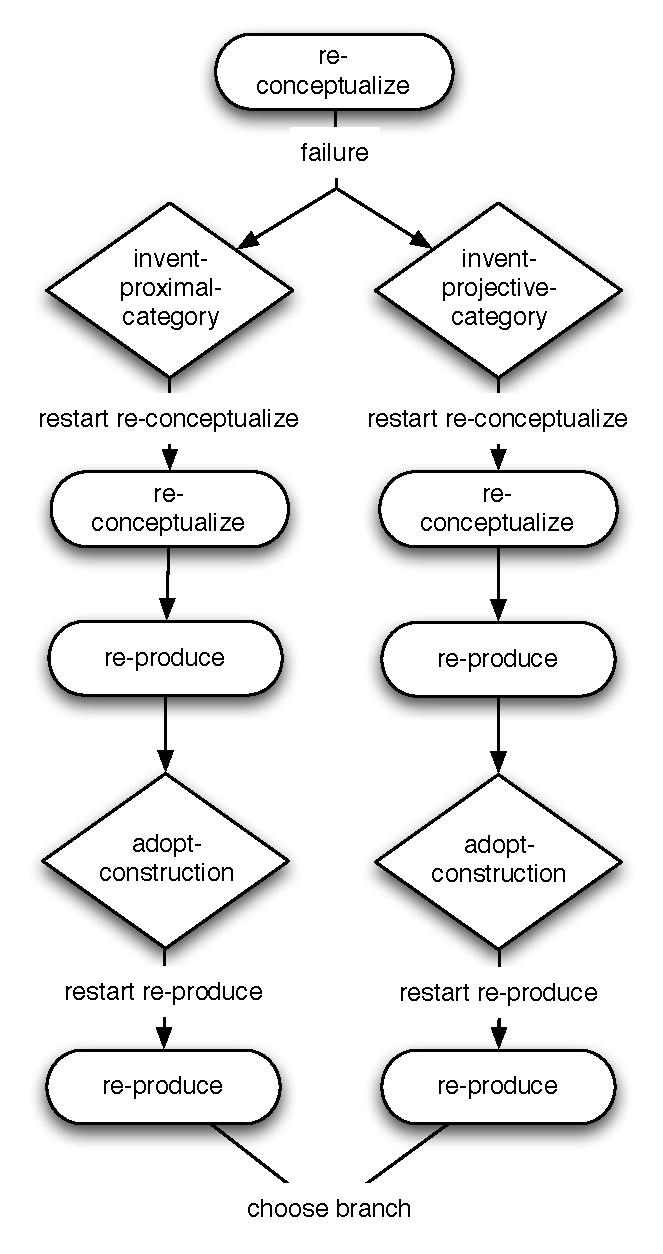
\includegraphics[width=0.5\columnwidth]{figs/re-production-branching}
\end{center}
\caption[Schematic flow of control when {\footnotesize\tt re-production} branches]{%
Schematic flow of control when {\footnotesize\tt re-production} branches to track
different possible inventions. If there is a failure in \emph{re-conceptualize} and
the agent is equipped with different strategies for solving this problem, the processing
splits into two branches. Here, the {\footnotesize\tt invent-proximal-category} learning operator
(part of the proximal language strategy) and the 
{\footnotesize\tt invent-projective-category} learning operator 
(part of the projective language strategy) both apply to 
fix the problem. Consequently, in each branch different
categories are invented and different constructions that 
link each category to the utterance are adopted.
At the end of processing the branch with the overall 
maximum score is chosen and the categories
and constructions of that task are saved by the agent.}
\label{f:re-production-branching}
\end{figure}


\begin{figure} 
\begin{center}
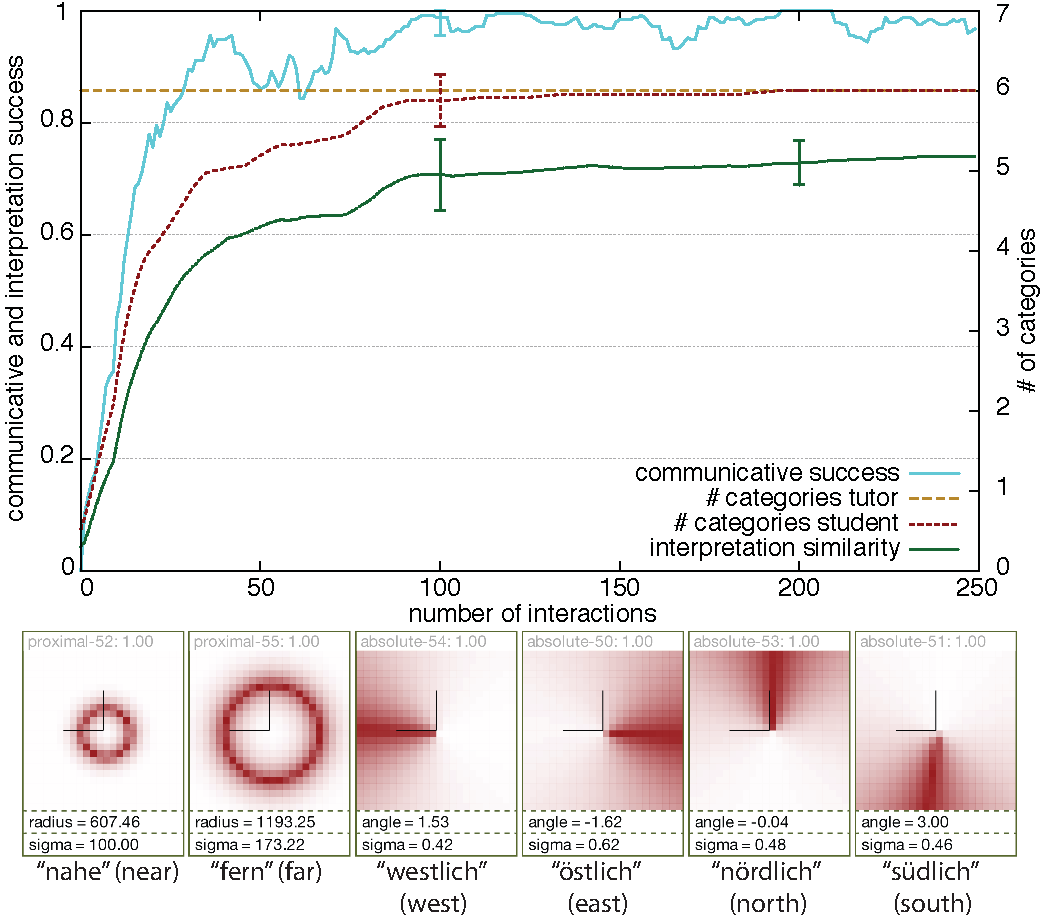
\includegraphics[width=0.7\columnwidth]{figs/category-acquisition-absolute+proximal-results+categories}\\
\vspace{0.1cm}
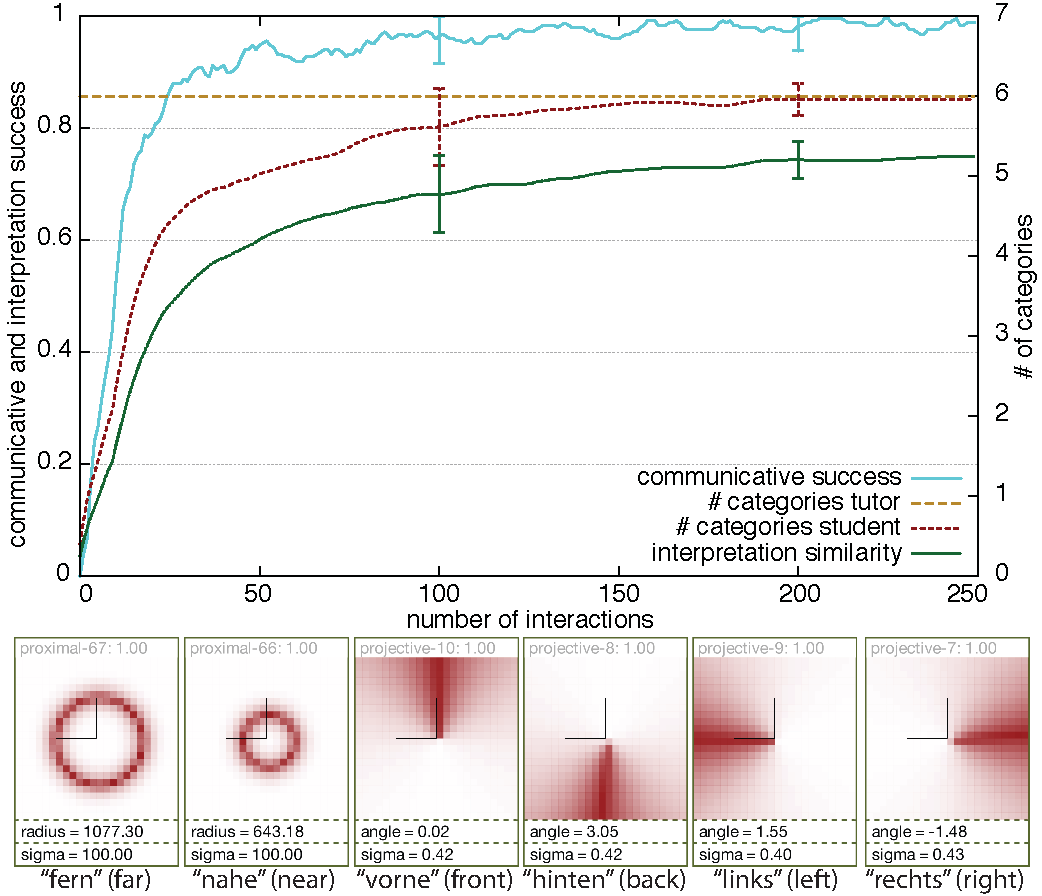
\includegraphics[width=0.7\columnwidth]{figs/category-acquisition-projective+proximal-results+categories}
\end{center}
\caption[Results for dual acquisition experiments]{Results for two types of acquisition experiments using inference. 
One in which the tutor is equipped with proximal and projective 
categories (top) and one where the tutor is  given proximal and 
absolute categories (bottom).}
\label{f:category-acquisition-proj+prox++abs+prox-results}
\end{figure}

The use of discrimination, fundamentally, rests on exploiting 
conceptualization as an inference process. The best of the three
different possible category types is chosen based on what is the most 
plausible category given that the tutor also choose the category based on 
the principle of maximizing discriminative power.
Figure \ref{f:category-acquisition-proj+prox++abs+prox-results} 
shows results both for an
acquisition experiment where the tutor is equipped with proximal 
and projective categories at the same time and
for a population in which the tutor is equipped with
absolute and proximal categories at the same time. 
In both cases the dynamics of acquisition are comparable 
to the single category type cases, although reaching the baseline 
success takes longer due to the increased number of categories\is{measures!number of categories}.
Learners quickly pick up the categories and are able to communicate 
successfully. Hence, the inference in conceptualization based on discrimination
scores is successful.

However, in certain combinations of category types using the 
principle of maximizing discriminative power has limits. 
Figure \ref{f:category-acquisition-projective+absolute-results} shows 
a case where the target language system
given to the tutor has both projective and absolute categories. We can observe
that the learner is unable to achieve similar communicative success as in all
other cases of acquisition discussed in this chapter. Second, learners also 
cannot advance in establishing interpretation similarity. Third, the categories
acquired by the learner are of the wrong type, as for example, \textit{westlich} (`west')
was acquired as a projective category rather than as an absolute one and \textit{rechts} (`right')
was adopted as absolute rather than projective category. Why is that?
A key to the answer can be found in Figure 
\ref{f:category-acquisition-absolute+proximal+projective-single-acquisition}. 
The problem is that in contexts where there is a global reference the learner
upon hearing a new word has no means to decide on whether a projective or 
absolute category was used. In the example described in that figure, both the invented 
absolute and the invented projective category have the same discrimination score, 
because both exclusively rely on the angle to the topic object. Now, the angle to the
topic object for both absolute and projective category may be different in numerical 
value for the invented absolute and projective categories, but their discriminative power 
is the same (0.11 in the case described by the figure). 
In other words, the discrimination score does not distinguish between both
the absolute and the projective systems in the same way as it does for the difference
of both to the proximal category. 

The reason why this problem appears in the particular constellation of this chapter is, of course, 
that both absolute and projective categories compete for the same angular dimension. 
If, for instance, the absolute categories would focus on a different angular dimension then
the projective ones this problem would not occur. Consider the 
example of \textit{über} (`above') and \textit{unter} (`below'), which have a 
predominantly absolute reading, but they focus on a
different direction than their horizontal counterparts. In this case the problem
does not appear and discrimination could do its job. Similarly, if there would 
be a strong tendency or bias in the population to use a certain type of category if applicable, 
the problem can also be alleviated. 
For the case discussed in this section one can for instance add a bias to all agents 
to prefer to use absolute categories over other ones if a global reference licensing 
their application is available. Figure 
\ref{f:category-acquisition-projective+absolute-biased-results}
shows the results of  an experiment in which all agents are equipped with such a bias.
The difference to the non-biased case in Figure \ref{f:category-acquisition-projective+absolute-results}
is obvious. Agents with bias can easily pick up the language system of their tutors. 
Biasing points to an additional layer of complexity which will be discussed in much
more detail in the coming sections. The bias for absolute conceptualizations 
is implemented by boosting particular
semantic structure used in conceptualization. Categories in conceptualization
are always part of some semantic structure that applies them to the current context.
These structures are necessarily different for different kinds of categories. A fact that
I hinted at already in much more detail in Section \ref{s:german-locative-phrases-semantic-processing}.
To introduce a bias, consequently, means to score semantic structure used for applying absolute categories
to the current context higher than those for projective and proximal categories.
Semantic structure, in particular, the operations used in conceptualization are 
themselves subject to acquisition and formation something which is discussed
in more detail in later sections. 


\begin{figure} 
\begin{center}
% \includegraphics[width=0.9\columnwidth]{figs/category-acquisition-projective+absolute-results+categories}
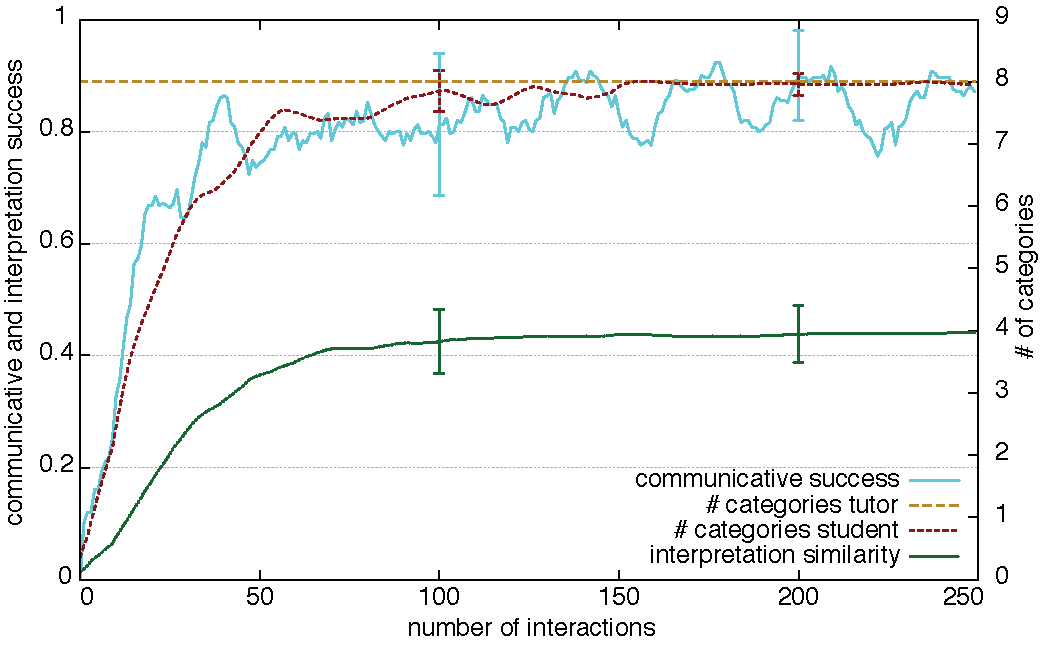
\includegraphics[width=0.8\columnwidth]{figs/category-acquisition-projective+absolute-results+categories-1}
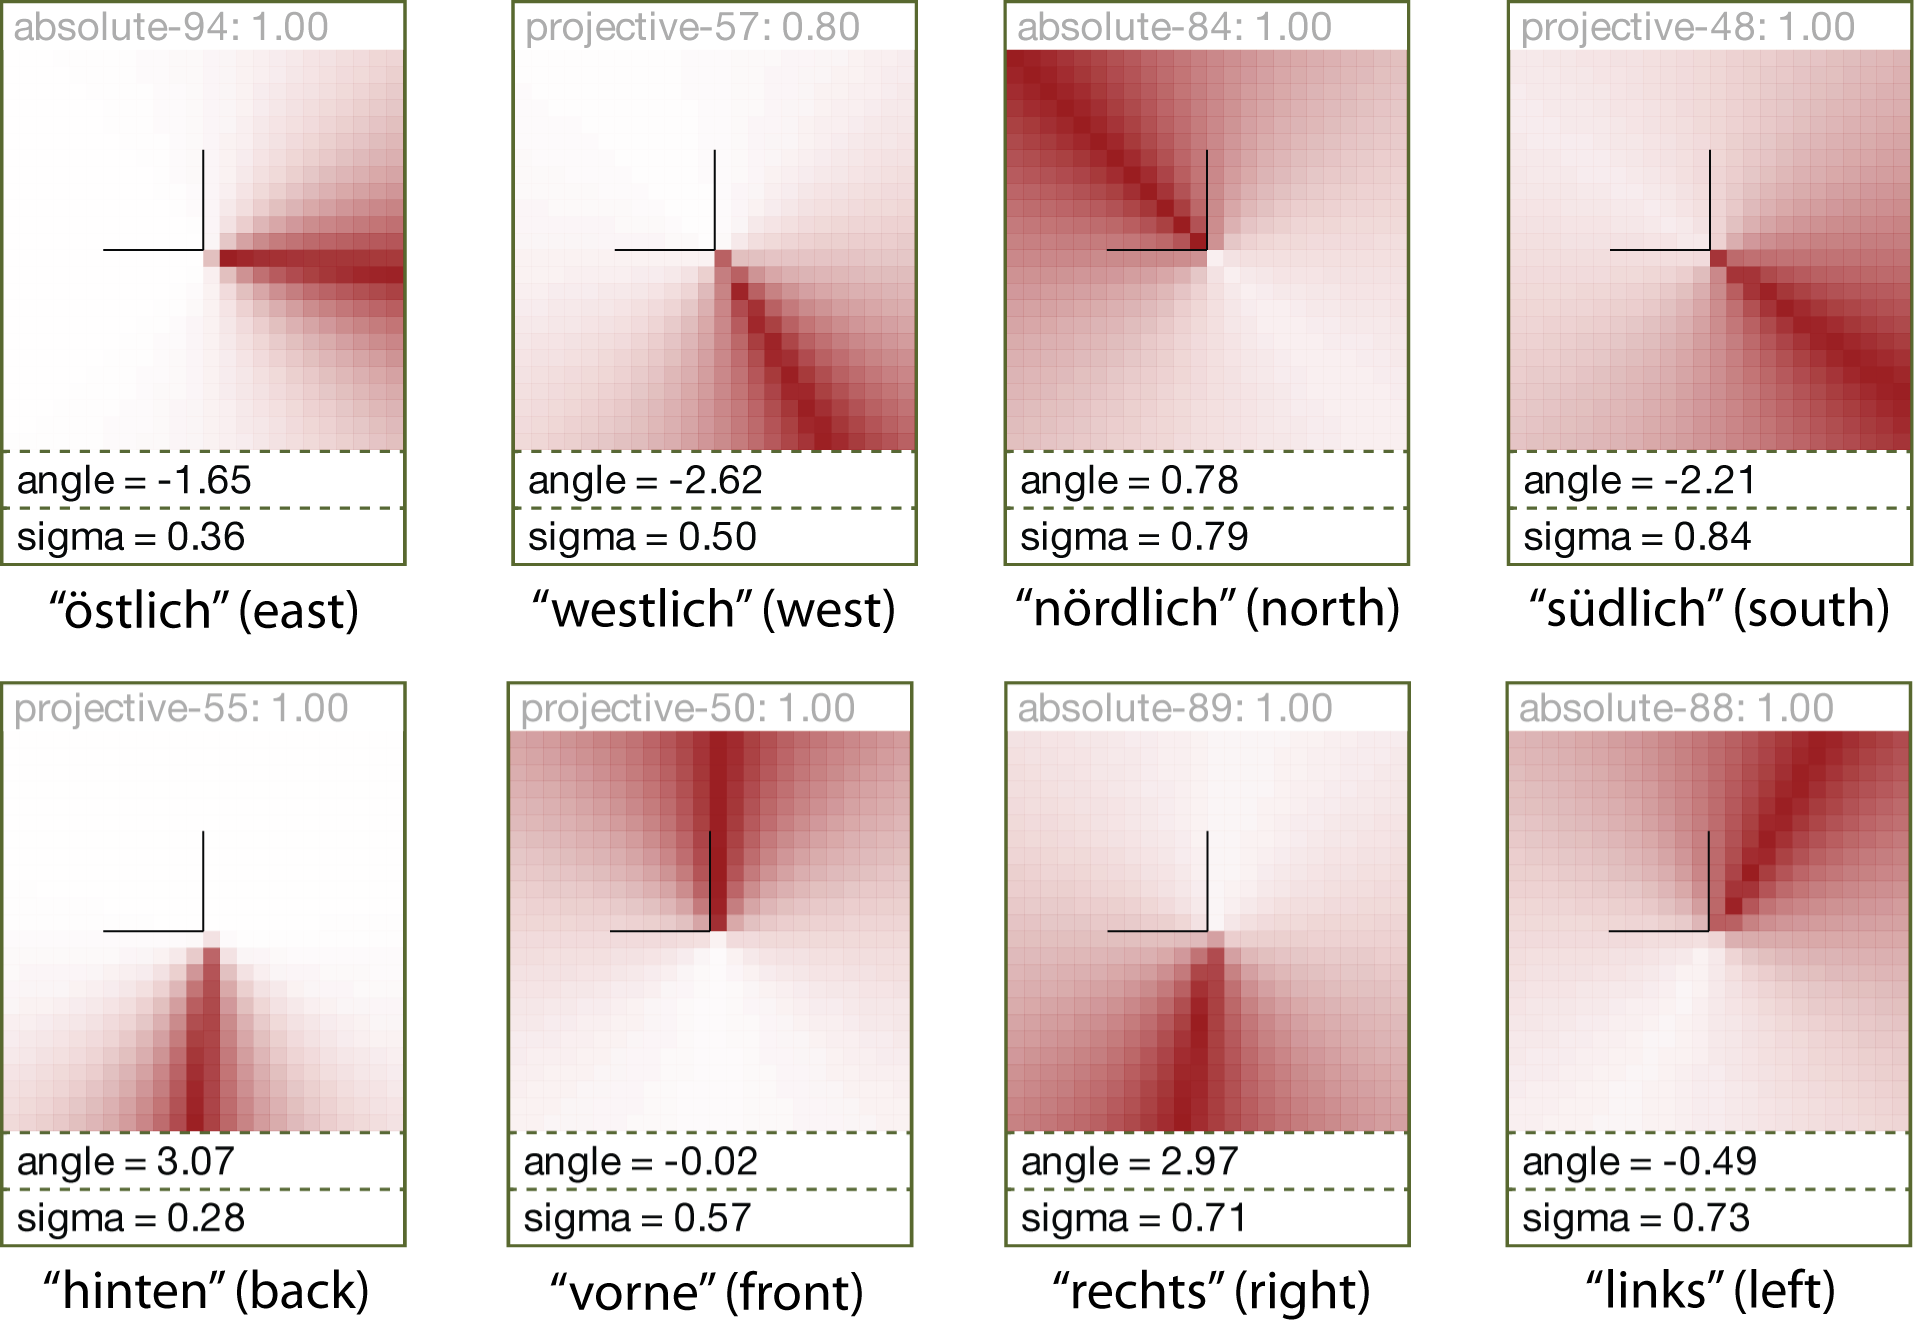
\includegraphics[width=0.8\columnwidth]{figs/category-acquisition-projective+absolute-results+categories-2.png}
\end{center}
\caption[Results for acquisition of projective and absolute systems]{%
Results for an acquisition experiment in which learners face 
the German projective and absolute language system at the same time. 
Learners have no means of determining the strategy, and therefore have 
to guess the strategy behind each word. The system that learners 
acquire differs from the tutor systems quite substantially, the estimated 
categories have few similarities with their target, and they are 
also of the wrong type (e.g. \textit{südlich} (`south') is learned as a projective category).
Communicative success\is{measures!communicative success} remains surprisingly high. 
However, a success rate of 80\% is low in comparison with other acquisition experiments.}
\label{f:category-acquisition-projective+absolute-results}
\end{figure}


\begin{figure} 
\begin{center}
% \includegraphics[width=0.9\columnwidth]{figs/category-acquisition-projective+absolute-biased-results+categories}
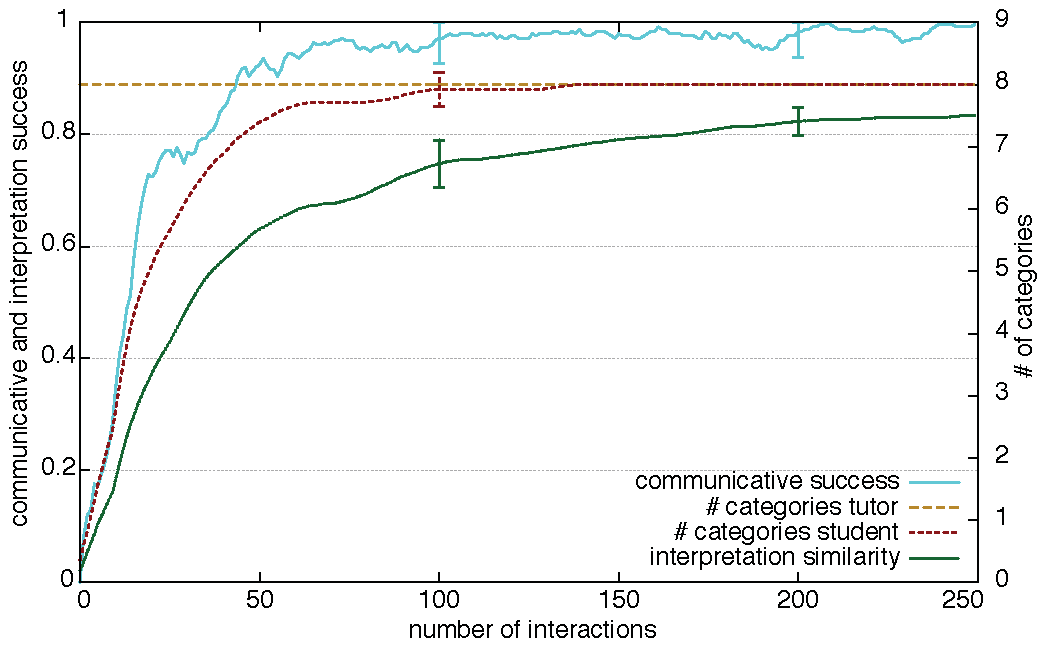
\includegraphics[width=0.8\columnwidth]{figs/category-acquisition-projective+absolute-biased-results+categories-1}
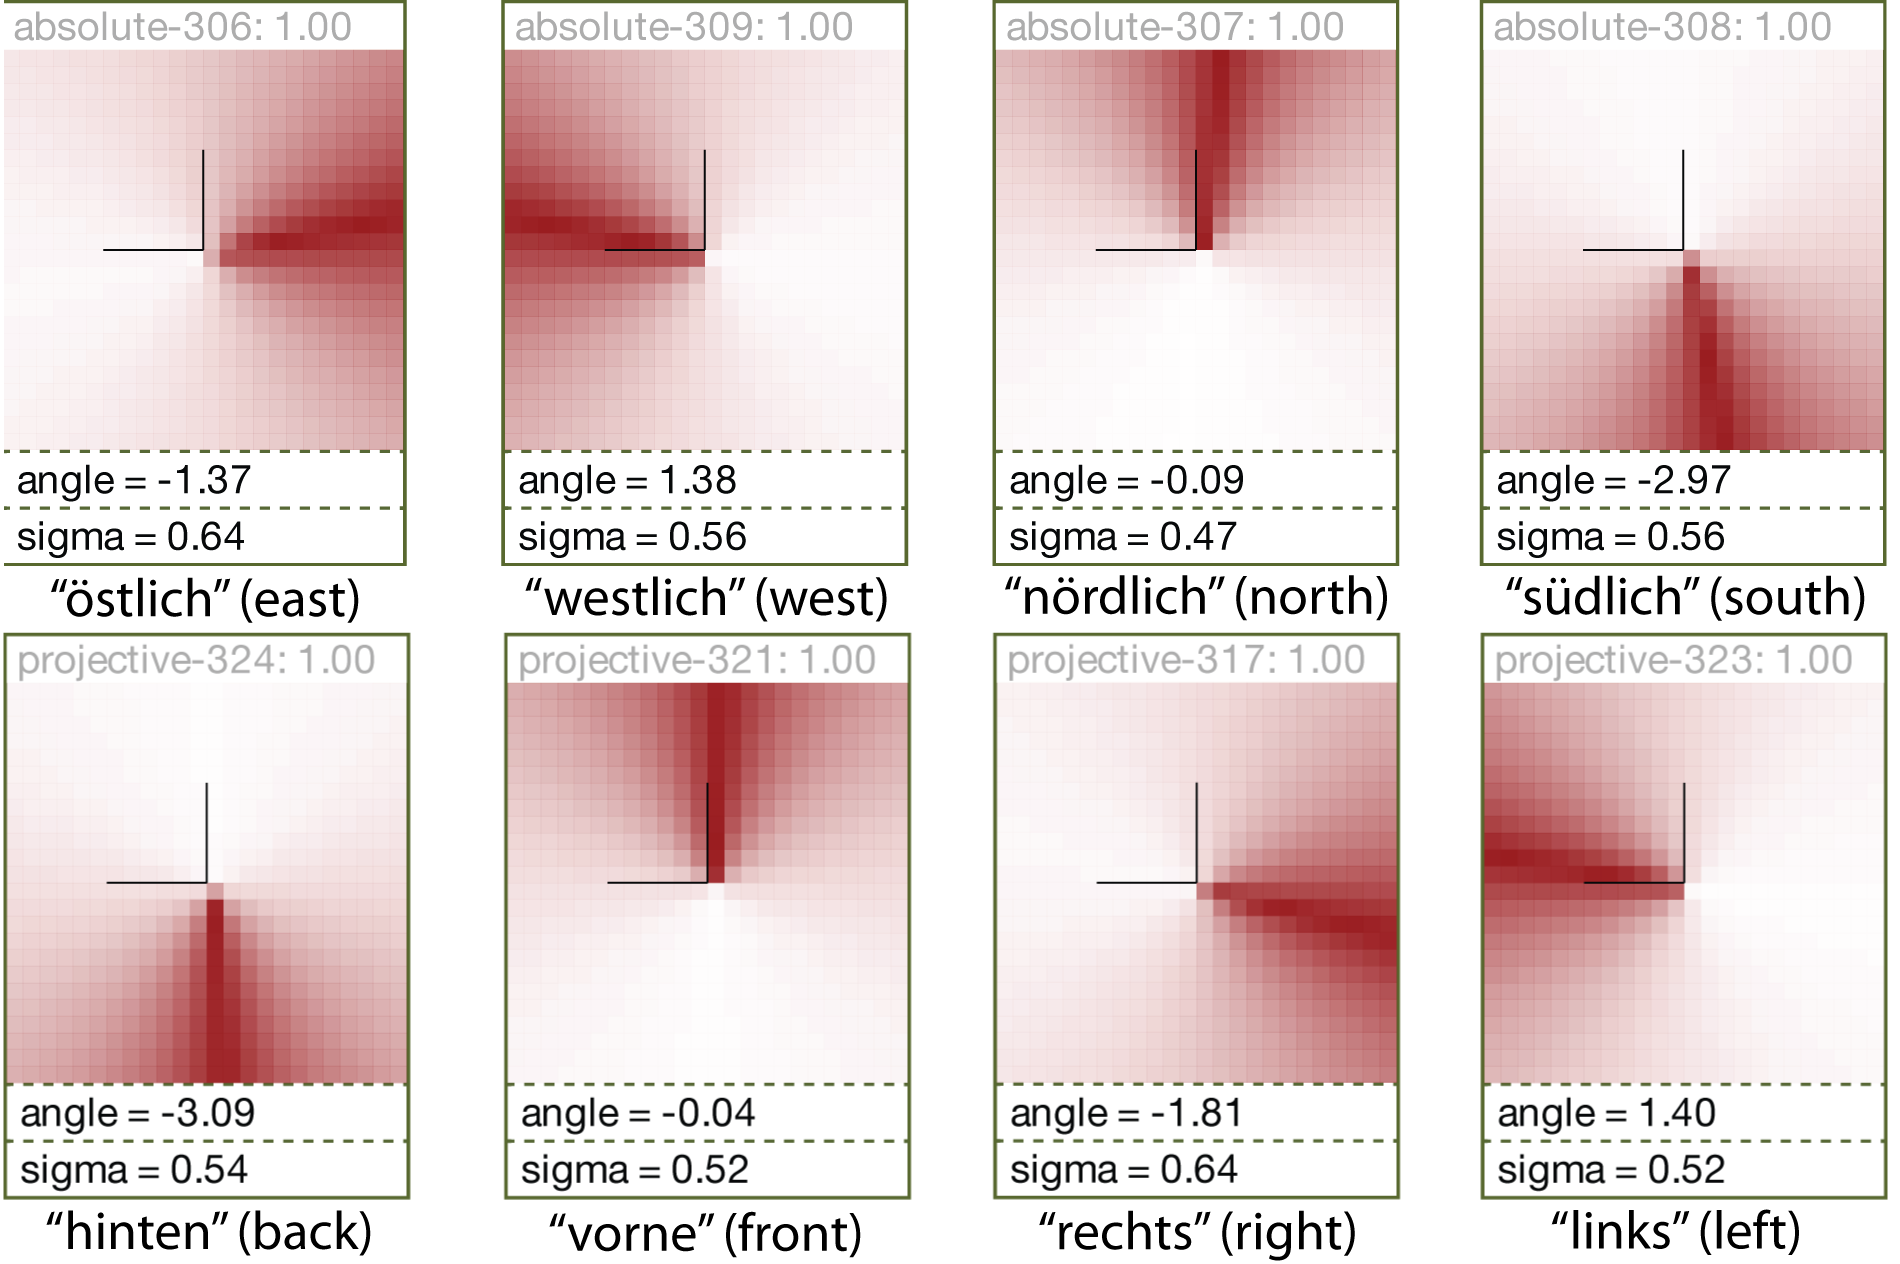
\includegraphics[width=0.8\columnwidth]{figs/category-acquisition-projective+absolute-biased-results+categories-2.png}
\end{center}
\caption[Preference based acquisition of proximal and absolute systems]{%
Results for an acquisition experiment where learners face 
both a projective and absolute system
at the same time. In contrast to the results shown in Figure \ref{f:category-acquisition-projective+absolute-results}, agents are equipped with a strong preference for the absolute strategy. If the environment
has absolute features agents prefer absolute conceptualizations of the spatial scene. 
Consequently, upon observing a new word in a context where absolute features are available, learners 
will adopt the word as part of an absolute language strategy. Based
on the bias, learners successfully and correctly acquire the complete system.}
\label{f:category-acquisition-projective+absolute-biased-results}
\end{figure}



\subsubsection{Hybrid systems}
Another extent in which all previous acquisition experiments are equal is that
in all of them learners are equipped with very particular mechanisms for 
each category type. A learner, for instance, in the case of a full language 
system encompassing absolute, projective and proximal categories is equipped 
with a separate learning mechanism for each 
category type. Let us for a moment put aside the problem of discriminating
between projective and absolute categories and focus only on the case of 
proximal and projective categories. The assumption that there is a separate
learning operator for each of these two in acquisition is an assumption that can be 
questioned, based on the grounds that it presupposes the existence
of learning operators for each particular input dimension, namely distance and angle. 
In this section I propose a mechanism in which such a bias for clear-cut 
channel distinctions is not given to a learner prior to acquiring
the language system, but in which the channel focus of certain categories
is autonomously established by the learner. The mechanism consists, first, of 
a representation that encompasses both distance and angle sensory channels and, second, 
an alignment mechanism for both distance and angle channels in categories.
The new category type is called \textsc{proximal-angular} and is essentially a combination
of the proximal and the angular category type. It consists of two channel values, 
distance $d$ and angle $a$, as well as corresponding sigma values for each channel
($\sigma_a$ and $\sigma_d$).
The similarity $\operatorname{sim}$ of some object to a 
particular proximal-angular category 
is computed as the product of angle and distance similarity.
\begin{eqnarray}
\label{e:proximal-angular-similarity}
\operatorname{sim}(l,c)&:=& \operatorname{sim_a}(l,c) \cdot \operatorname{sim_d}(l,c)
\end{eqnarray}
In the above formula $\operatorname{sim_a}$ is the similarity defined for  angular categories 
(see Equation \ref{e:angular-category-similarity}) and $\operatorname{sim_d}$ is defined
as the similarity for proximal categories (see Equation \ref{e:proximal-category-similarity}).

\begin{figure}
\begin{center}
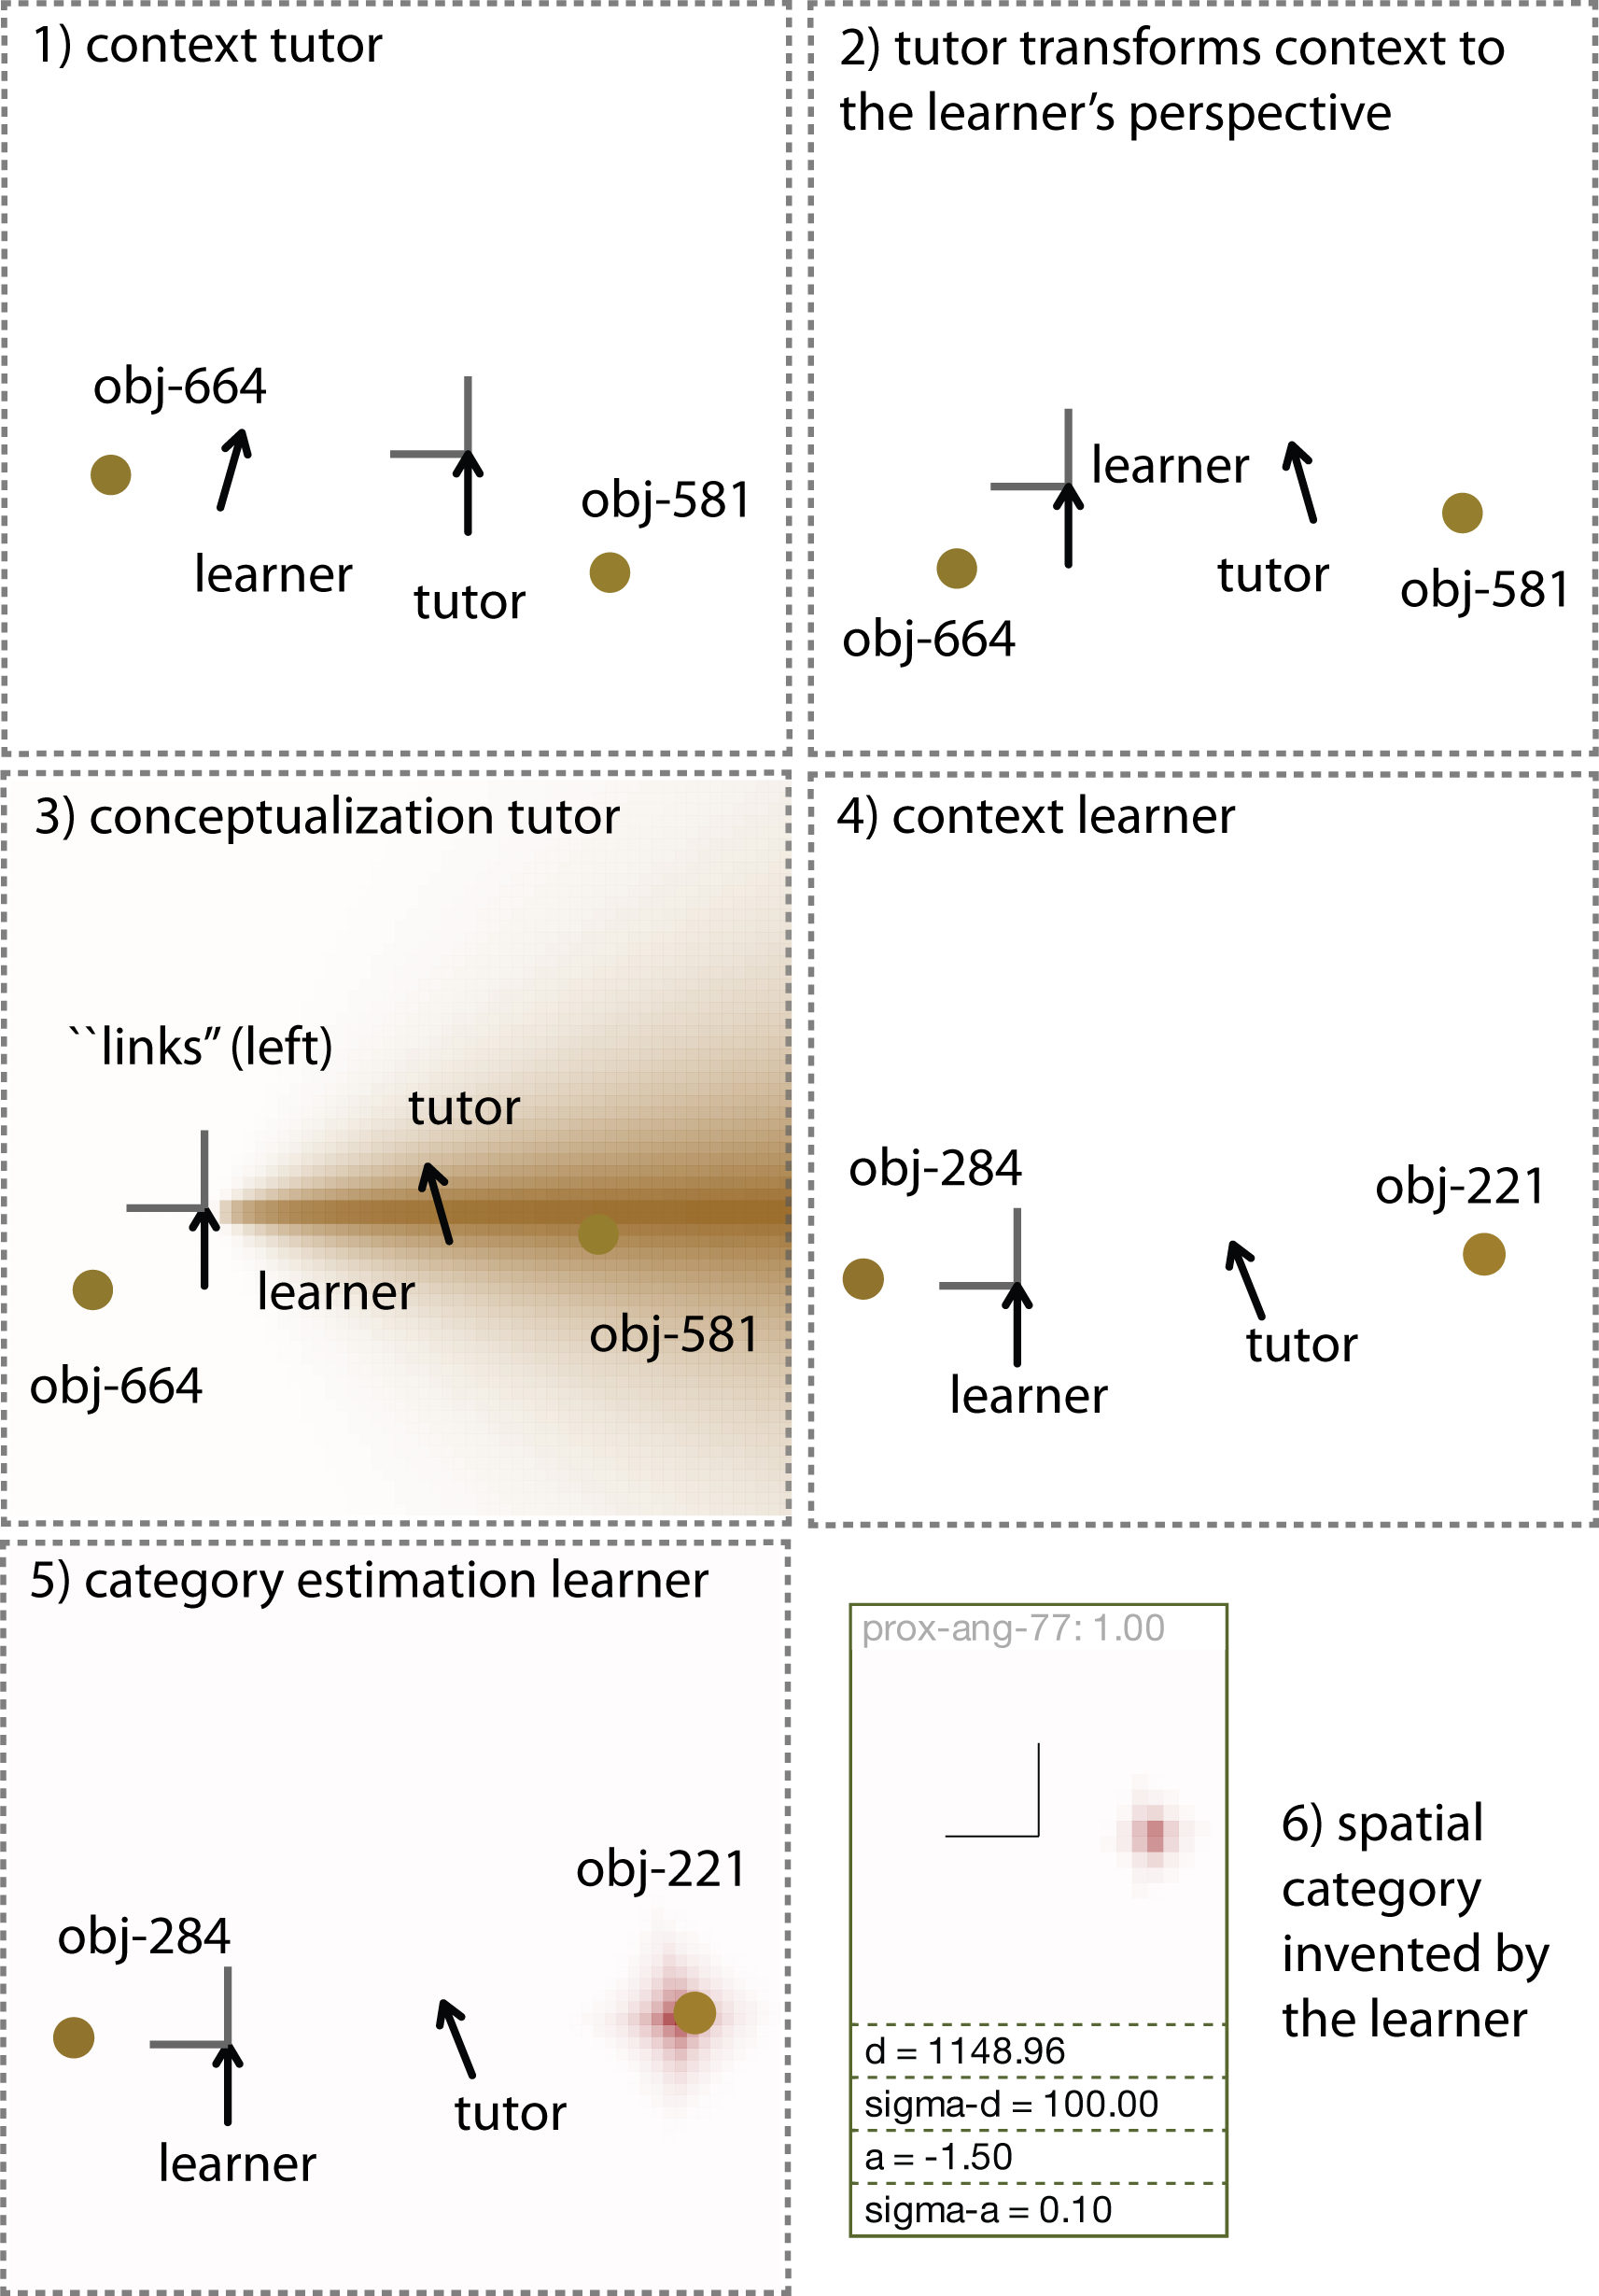
\includegraphics[width=0.8\columnwidth]{figs/category-acquisition-proximal-angular-single-category-acquisition.png}
\end{center}
\caption[Acquisition of a single {\footnotesize\tt proximal-angular} category]{Acquisition of a single {\footnotesize\tt proximal-angular} category. The steps are the same 
as for proximal, projective and absolute category adoption, except for the resulting category 
which is focussed around the topic object ({\footnotesize\tt obj-581} in the tutor's context and
{\footnotesize\tt obj-221} in the learner's context) both in terms of angle and direction.
Initial sigma values both for the angular and the distance dimension 
($\sigma_d$ and $\sigma_a$) are small.}
\label{f:category-acquisition-proximal-angular-single-category-acquisition}
\end{figure}

\begin{figure}
\begin{center}
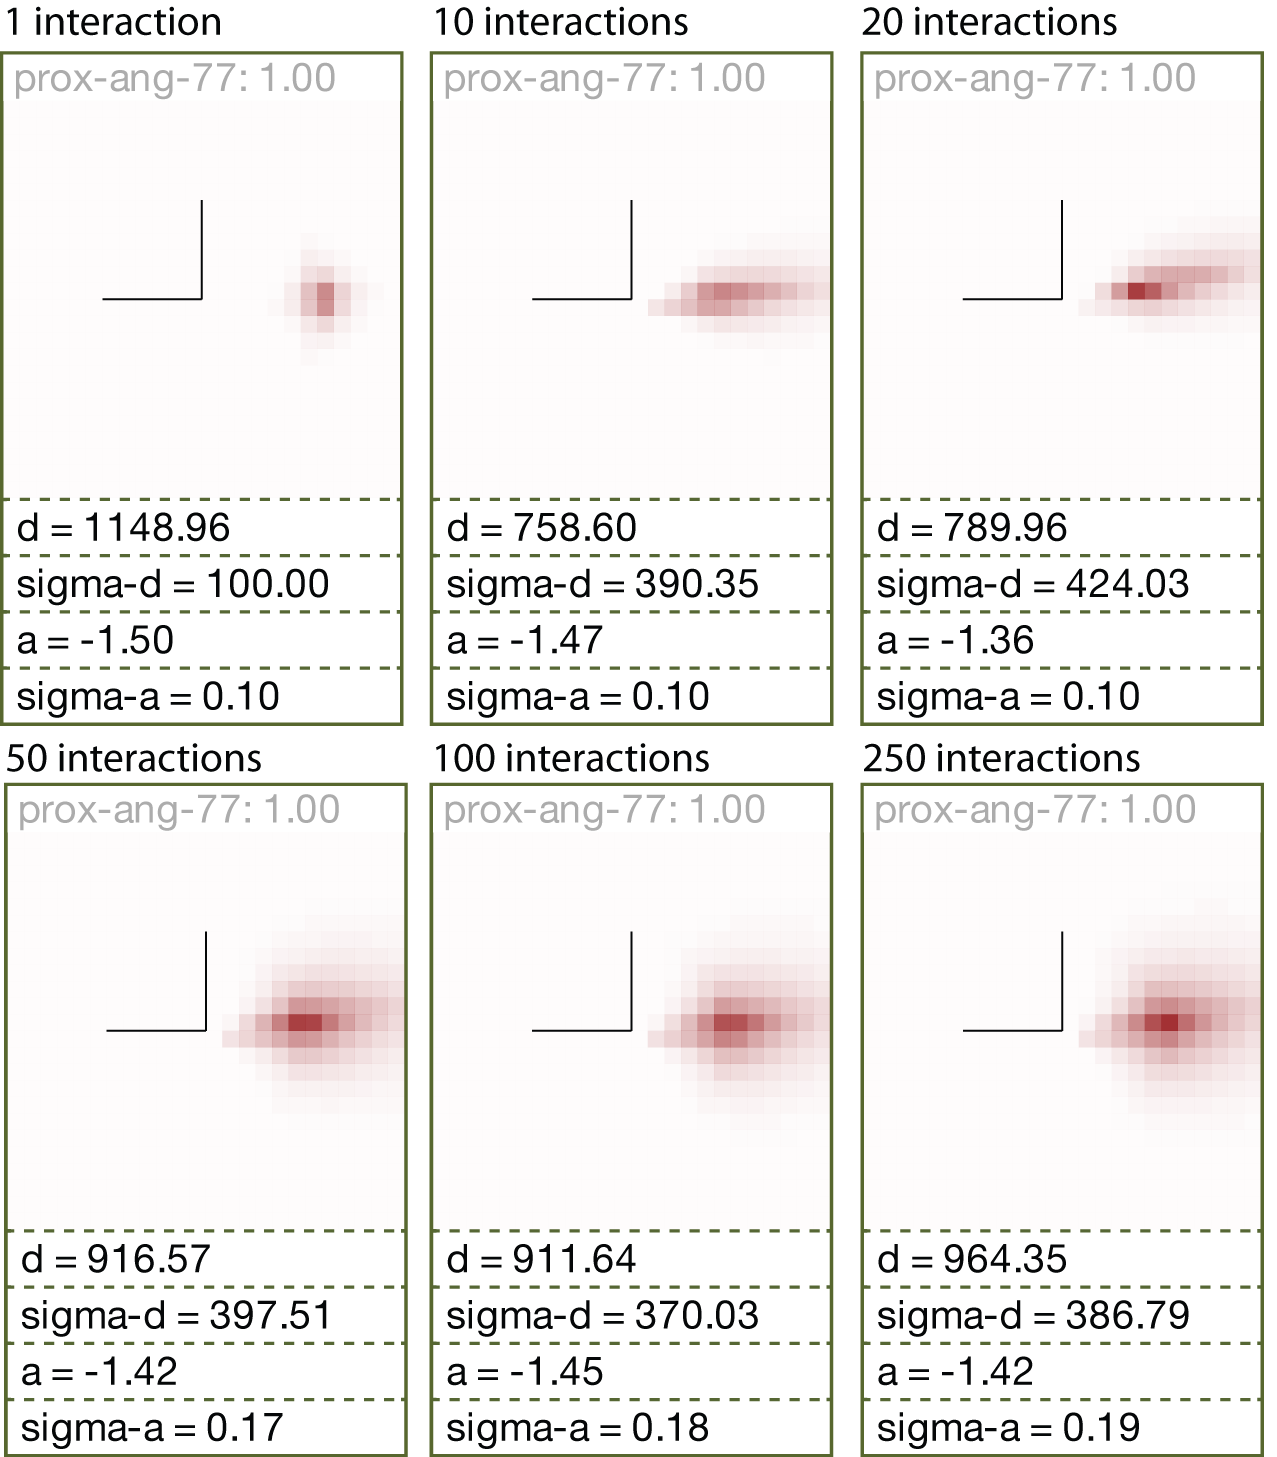
\includegraphics[width=0.9\columnwidth]{figs/category-acquisition-proximal-angular-category-development-over-time.png}
\end{center}
\caption[Development of a single {\footnotesize\tt proximal-angular} category over time]{%
Development of a single {\footnotesize\tt proximal-angular} category over time (see Figure \ref{f:category-acquisition-proximal-angular-single-category-acquisition} for the initial invention of that category). 
Over the course of many interactions this category which is linked to the word \textit{links} (`left') develops
into a category which resembles more and more the projective category {\footnotesize\tt left}. 
The activation area is spread out in the distance dimension and more narrow in the angular 
dimension signified by a low $\sigma_a$ value and a high $\sigma_d$ value.}
\label{f:category-acquisition-proximal-angular-category-development-over-time}
\end{figure}

\begin{figure}
\begin{center}
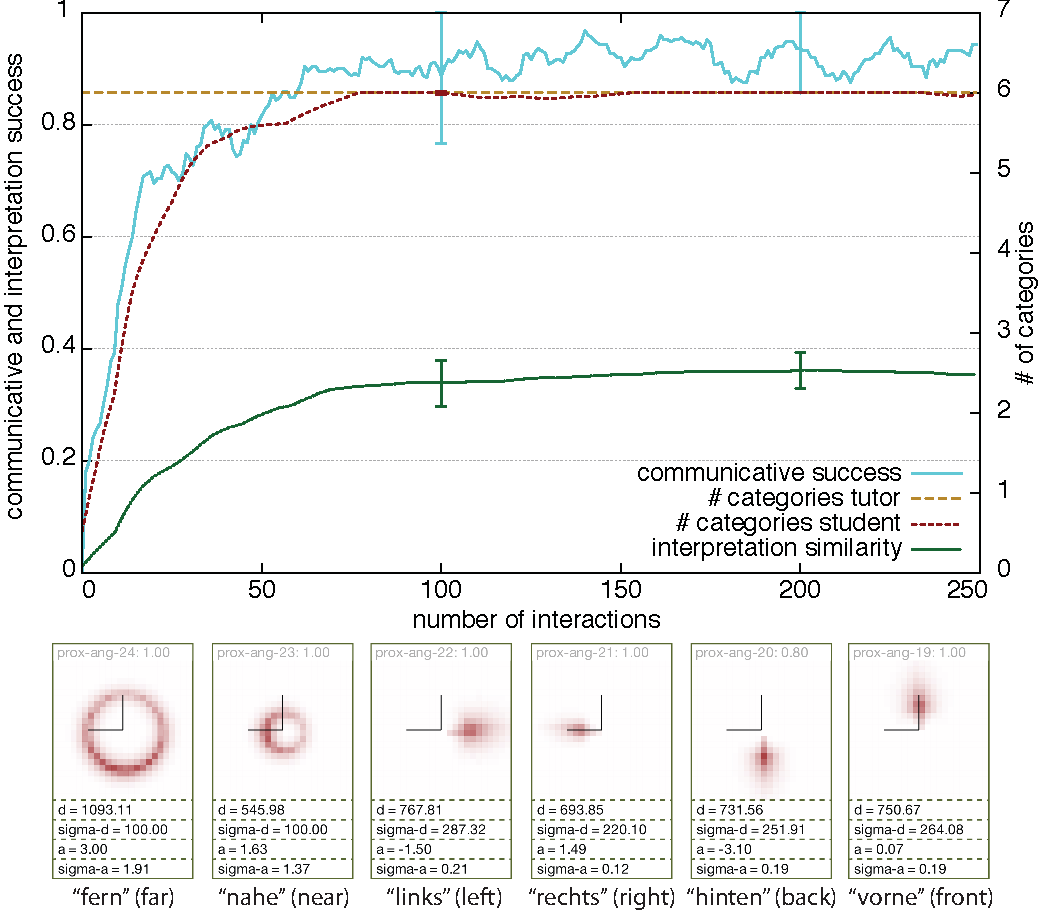
\includegraphics[width=0.9\columnwidth]{figs/category-acquisition-proximal-angular-results+categories}
\end{center}
\caption[Results for proximal-angular acquisition experiments]{%
Results for proximal-angular acquisition experiments in which the tutor
is given proximal and projective categories (25 runs averaged). Learners are 
equipped with proximal-angular category invention and alignment operations.
Communicative success\is{measures!communicative success} is more varied than in the case for single category acquisition.
Nevertheless, agents manage to learn words and category mappings, but the shape 
of the categories, i.e., their preferred activation, mirrors the categories given to tutors. 
Overall, interpretation similarity stays rather low which is mostly due to the differences 
in distance and sigma distance of the acquired categories. The reason is the same as
for proximal acquisition and lies in the distribution of object distances in the spatial scenes. 
The most important fact about interpretation similarity\is{measures!interpretation similarity} is that it stabilizes over time.}
\label{f:category-acquisition-proximal-angular-results}
\end{figure}

The category representation, thus, does not really introduce something 
new apart from the combination of two known representations. The similarity in 
representation carries over to the invention operator which is a combination of 
the invention operator for angular and proximal categories 
(see Figure \ref{f:category-acquisition-proximal-angular-single-category-acquisition} 
for an example of the acquisition of a single proximal-angular category).
When a proximal-angular category is invented by the learner it does not cover just a
particular channel. In fact, the invented category covers a small area both 
in angle and distance around the topic object. How the category develops after it has been invented is essentially a matter of the kind of objects which are successfully conceptualized and
interpreted using the category. The alignment operator after each interaction adds more samples 
to the category and recomputes the distance $d$ 
and the distance sigma $\sigma_d$ exactly like for proximal categories
(see Equations \ref{e:update-d} and \ref{e:update-sigma-d}) and 
the angle $a$ and the angle sigma $\sigma_a$ as for projective categories 
(see Equations \ref{e:update-a} and \ref{e:update-sigma-a}). 
Consequently, if more distance variation is acceptable
in the topic objects, the category's $\sigma_d$ (the distance channel sigma) 
can widen, in other words, the category is more discriminating in the angle direction. 
Vice versa, if topic objects are more angle varied then the category can 
develop into a more distance discriminating category. Figure 
\ref{f:category-acquisition-proximal-angular-category-development-over-time} shows how 
the category whose adoption is shown Figure \ref{f:category-acquisition-proximal-angular-single-category-acquisition} exemplarily develops over time. 

Figure \ref{f:category-acquisition-proximal-angular-results} 
shows the results for acquisition experiments with proximal-angu\-lar 
categories. The tutor in these experiments is simultaneously 
equipped with the German proximal and projective system. 
The learner is given adoption and alignment operators for proximal-angular 
categories. Overall communicative success stays slightly lower than in comparable experiments
(for instance, Figure \ref{f:category-acquisition-proj+prox++abs+prox-results} for acquisition of
proximal and projective categories). However, the task is also slightly
more difficult as agents have to acquire not only the mean values for distance \textit{and} angle of a
category, but also their distributional properties in the two sensory channels.

The way that the proximal-angular categories are implemented presupposes a particular
way of applying the angular component. In the experiments discussed in this section
the angular component was implemented to mirror projective categories. 
Technically speaking, one could have also chosen to use proximal-angular
categories with an angular component that operates like an absolute category by
taking into account the global features of the environment. Consequently, 
the problem of learning the absolute system at the same time as the projective system 
was left unexamined. In fact, the reasons for why this is even a problem apply 
just as drastically as they did before. Better answers will be given later sections.

\subsection{Implementation details}
In the above description I have glossed over some of the technical details. 
Specifically I have not explained how precisely the different conceptualization 
strategies are implemented. This section presents a simplified approach to spatial
conceptualization which will gradually be extended in the next chapters
to reach the full semantic complexity needed for spatial language.
Figure \ref{f:categorization-strategies} shows the IRL-network
used to implement the projective and the proximal strategy. The cognitive
operations {\footnotesize\tt identify-object-proximal} and  {\footnotesize\tt identify-object-projective}
implement the different categorization strategies. They are applied to an 
input set which for the learner is just the spatial context introduced by 
{\footnotesize\tt get-context}. These operations are not only used by the tutor to apply German 
spatial relations, but they also serve the learner in invention. 

\definition{Semantic Operation}{identify-object-proximal}
\begin{explanation}{description}
Applies a proximal category to an input set and extracts the 
object with the highest discrimination score.
\end{explanation}
\begin{explanation}{arguments}
{\footnotesize\verb+?identified-object+} (of type object) \\
{\footnotesize\verb+?source-set+} (of type entity-set) \\
{\footnotesize\verb+?category+} (of type proximal-category)
\vspace{0.3cm}
\end{explanation}

\definition{Semantic Operation}{identify-object-projective}
\begin{explanation}{description}
Applies a projective category to an input set and extracts the 
object with the highest discrimination score.
\end{explanation}
\begin{explanation}{arguments}
{\footnotesize\verb+?identified-object+} (of type object) \\
{\footnotesize\verb+?source-set+} (of type entity-set) \\
{\footnotesize\verb+?category+} (of type projective-category)
\vspace{0.3cm}
\end{explanation}

\section{Lexicon formation}
\label{s:category-formation}\is{lexicon!formation}
% from acquisition to formation
% speakers solve communicative problems through invention and adoption
% agents are equipped with adoption operators
From the acquisition of a lexical language system to the autonomous formation
of a lexical language it is only a small step. In fact, in many ways the 
whole process of adopting a particular lexical item is already one 
of invention because learners invent categories 
based on the topic object and the current context followed by the invention of 
constructions that link some observed word to the invented category. 
Consequently much of the machinery for acquisition can be
used for formation, the only difference being that the word to which a category
is linked via a construction is not perceived by a learner but itself invented by agents. 
However, while there are some striking similarities, there are also some important differences. 
The most important of which is that formation is necessarily happening in a population of agents that
is larger than two agents. This puts particular pressure on alignment\is{alignment} operations as 
different words might pop up in a population for the same concept, but also 
since the categories themselves can diverge into different
corners of the conceptual space within the population. All of this is caused by the
fact that all interactions of agents are local involving always only
two agents of the population. Any kind of agreement two agents
reach, whether it is to use a certain word or to apply a certain category, consequently,
requires adoption and alignment across the population.

% close up invention
When forming a language system, speakers, at least in the beginning, lack the proper
categories to conceptualize reality and/or the proper linguistic means to express 
themselves. For instance, when an agent encounters an object that he cannot 
discriminate the categories known to him, the interaction fails. 
Now if no one in the population ever does anything about this problem,
there will obviously be no communication. Hence, in contrast to acquisition where
the learner being unable to conceptualize can wait until he picks up new semantic 
distinctions from the tutor, speakers in forming a language system are forced to resolve
their problems by inventing distinctions themselves. The learning operators used in formation, however,
are not that different from acquisition. Given some topic object, speakers
are given the ability to invent a category comparable to the cases discussed in acquisition 
in Section \ref{s:category-acquisition}. If there is a problem diagnosed in conceptualization, 
for instance, if the speaker cannot discriminate the topic object or 
he cannot discriminate it enough, i.e. the discrimination score of the best 
conceptualized meaning is too low, he can repair the problem
by creating a new category based on the topic object. This solves his problem 
in conceptualization. If he then goes on to try and produce an utterance for the newly created
category, he will face the problem that he has no means to express himself. The category
was just invented and, hence, there are no constructions linked to the category yet. He
resolves this problem by applying another repair strategy that of inventing a
new word together with a lexical construction that links the new category with the new word.
Given that the hearer is equipped with the same operators as learners in acquisition, he can pick
up both the newly invented word, as well as invent a category that is very similar
to the one of the speaker. 

% close up alignment
After such an interaction, two agents of the population have reached consensus about \is{alignment}
how to name a particular direction or distance, but this knowledge is still local to the two
agents that have participated in the interaction. The newly invented string as well
as the category now have to stand the test of time and they have to become
adopted and shared in the population. The process of alignment on the 
population level is one in which the category can undergo change and adoption
by agents in the population. It is particularly important to realize that 
in contrast to acquisition the target system is not fixed, in fact, it is unclear what
the target system is and agents can freely develop the system and adapt it to
their needs. The most important issue when adapting a language system is 
then, besides finding a suitable set of category distinctions and words to denote
these distinctions, is to reach consensus on the population level. Alignment
works on all levels of processing. The score of categories and constructions used in 
conceptualization or interpretation is updated based on the success of the interaction.
The shape of categories used in production and interpretation is updated by 
adding another sample and re-estimating the particular distance or angle
of the category (same as described in Section \ref{s:category-acquisition}).

\subsection{Experimental setup}
I test the validity of this approach to formation by running experiments 
in which typically 10 agents start without any categories and constructions 
and gradually have to solve their communicative problems by invention and
adoption of linguistic and semantic material. A set of measures tracks the 
progress of the population in establishing a communication system. The
measures are the same as for acquisition (communicative success,
number of categories and interpretation similarity), except that 
the average \emph{number of constructions}\is{measures!number of constructions} in the population is also tracked, 
because the mapping between categories and constructions is not necessarily one
to one due to synonymy. Also, the number of categories\is{measures!number of categories} is
not separately tracked for tutors and students but averaged across the population, 
because the distinction into tutor and learner agents does not exist in formation 
experiments. Every agent has the same capacity to invent and adopt \is{measures!interpretation similarity}
constructions and categories. Consequently, the interpretation similarity 
measure is averaged over all agents and all words in the population.


Spatial language necessarily is always tight to a particular reference system which
is to say every spatial relation is always applied with respect to some
object. Even uttering single words like \textit{links} (`left') entails an implicit reference
system and the object discriminated by uttering this word depends at least on which
of the two interlocutors is used as reference object. In acquisition this problem 
was solved by the tutor who always conceptualized from the learner, and, hence, 
the implicit reference system in every communication was the learner. In formation
this problem occurs again. Agents can use themselves implicitly as reference points
or they can use additional reference objects available to them in the spatial
scene they are confronted with. A detailed discussion of these
problems and their impact on lexical development is deferred to later sections. 
In order to focus only on lexical development, the problem is solved here by 
always using the box which is available in all spatial
contexts used in this section as the reference object. Different categorization 
strategies are, thus, represented using different semantic structure which all 
involve the box in each context (see Figure \ref{f:categorization-strategies} for
details).

\begin{figure}
\begin{center}
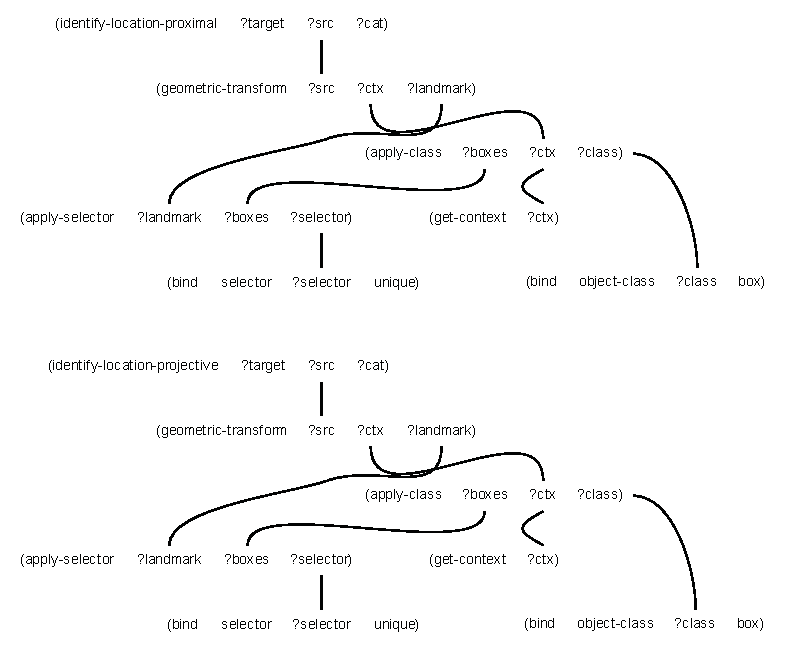
\includegraphics[width=1.0\columnwidth]{figs/category-formation-categorization-strategies}
\end{center}
\caption[Example strategies used in conceptualization]{%
Semantic structure used by agents to conceptualize reality. The top figure
shows the IRL-network for the projective strategy, the bottom figure for
comparison shows the proximal categorization strategy. Both differ in 
the categorization operation {\footnotesize\tt identify-object-projective} and
{\footnotesize\tt identify-object-proximal}. The rest of the network
transforms the complete context to the box landmark using the operation 
{\footnotesize\tt geometric-transform}.}
\label{f:categorization-strategies}
\end{figure}

\subsection{Results}
I test the invention and adoption system separately for absolute, proximal and
projective language strategies. Figures \ref{f:category-formation-projective-results}, 
\ref{f:category-formation-proximal-results} 
and \ref{f:category-formation-absolute-results} show both the communicative success\is{measures!communicative success}
averaged over 25 runs as well as examples of resulting language systems for
projective, proximal and absolute systems each. The graphs convincingly 
demonstrate the power of the invention and alignment operators, in other words, 
they show that given the proposed operators agents can develop a language
system and reach communicative success. Furthermore, these graphs show
that the language system evolved by agents is not necessarily the same
as the German language system. For instance, the categories of agents 1 to 3
in Figure \ref{f:category-formation-projective-results} are quite different from the 
German {\footnotesize\tt front}, {\footnotesize\tt back}, {\footnotesize\tt left} and {\footnotesize\tt right} projective
system which aligns its categories with the $x$ and $y$ axes of the coordinate system.
In particular, three categories seem to be sufficient for the agents in these experiments 
to discriminate all objects in the spatial scenes successfully. So the main question
given that we have established the success of the invention and alignment operators in formation 
is: what are the different factors influencing the shape of the language system developed?

Within the approach given in this book, there are two factors influencing the 
development of the category system which merit close consideration when 
it comes to explaining the outcome of formation experiments. 
First, the language strategy most importantly encompassing the conceptualization 
strategy as well as the learning and invention mechanisms including the 
set of parameters that come with them effect the forming language system. 
This is most obvious for the type of categories, e.g. absolute, projective or proximal, 
agents use for developing the language system because this entirely determined by
the strategy. The second important factor are the particular spatial scenes and their
properties that agents need to communicate in. The spatial scenes and the statistical 
distribution of objects are directly linked to the categories necessary for
discriminating objects.

\begin{figure}
\begin{center}
% \includegraphics[width=0.9\columnwidth]{figs/category-formation-projective-results+categories}
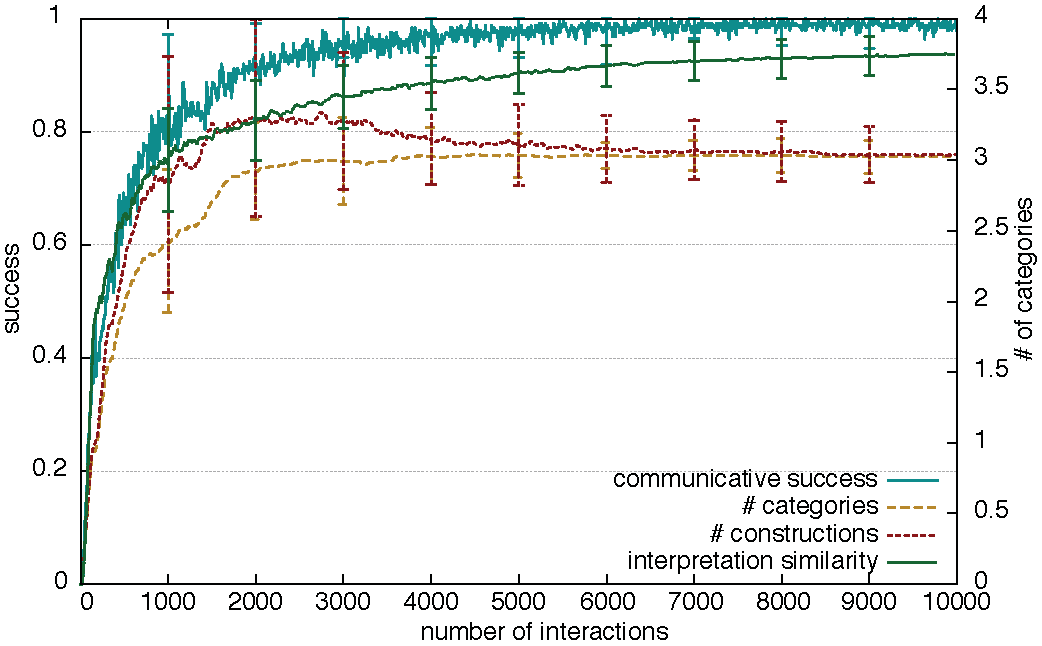
\includegraphics[width=0.9\columnwidth]{figs/category-formation-projective-results+categories-1}
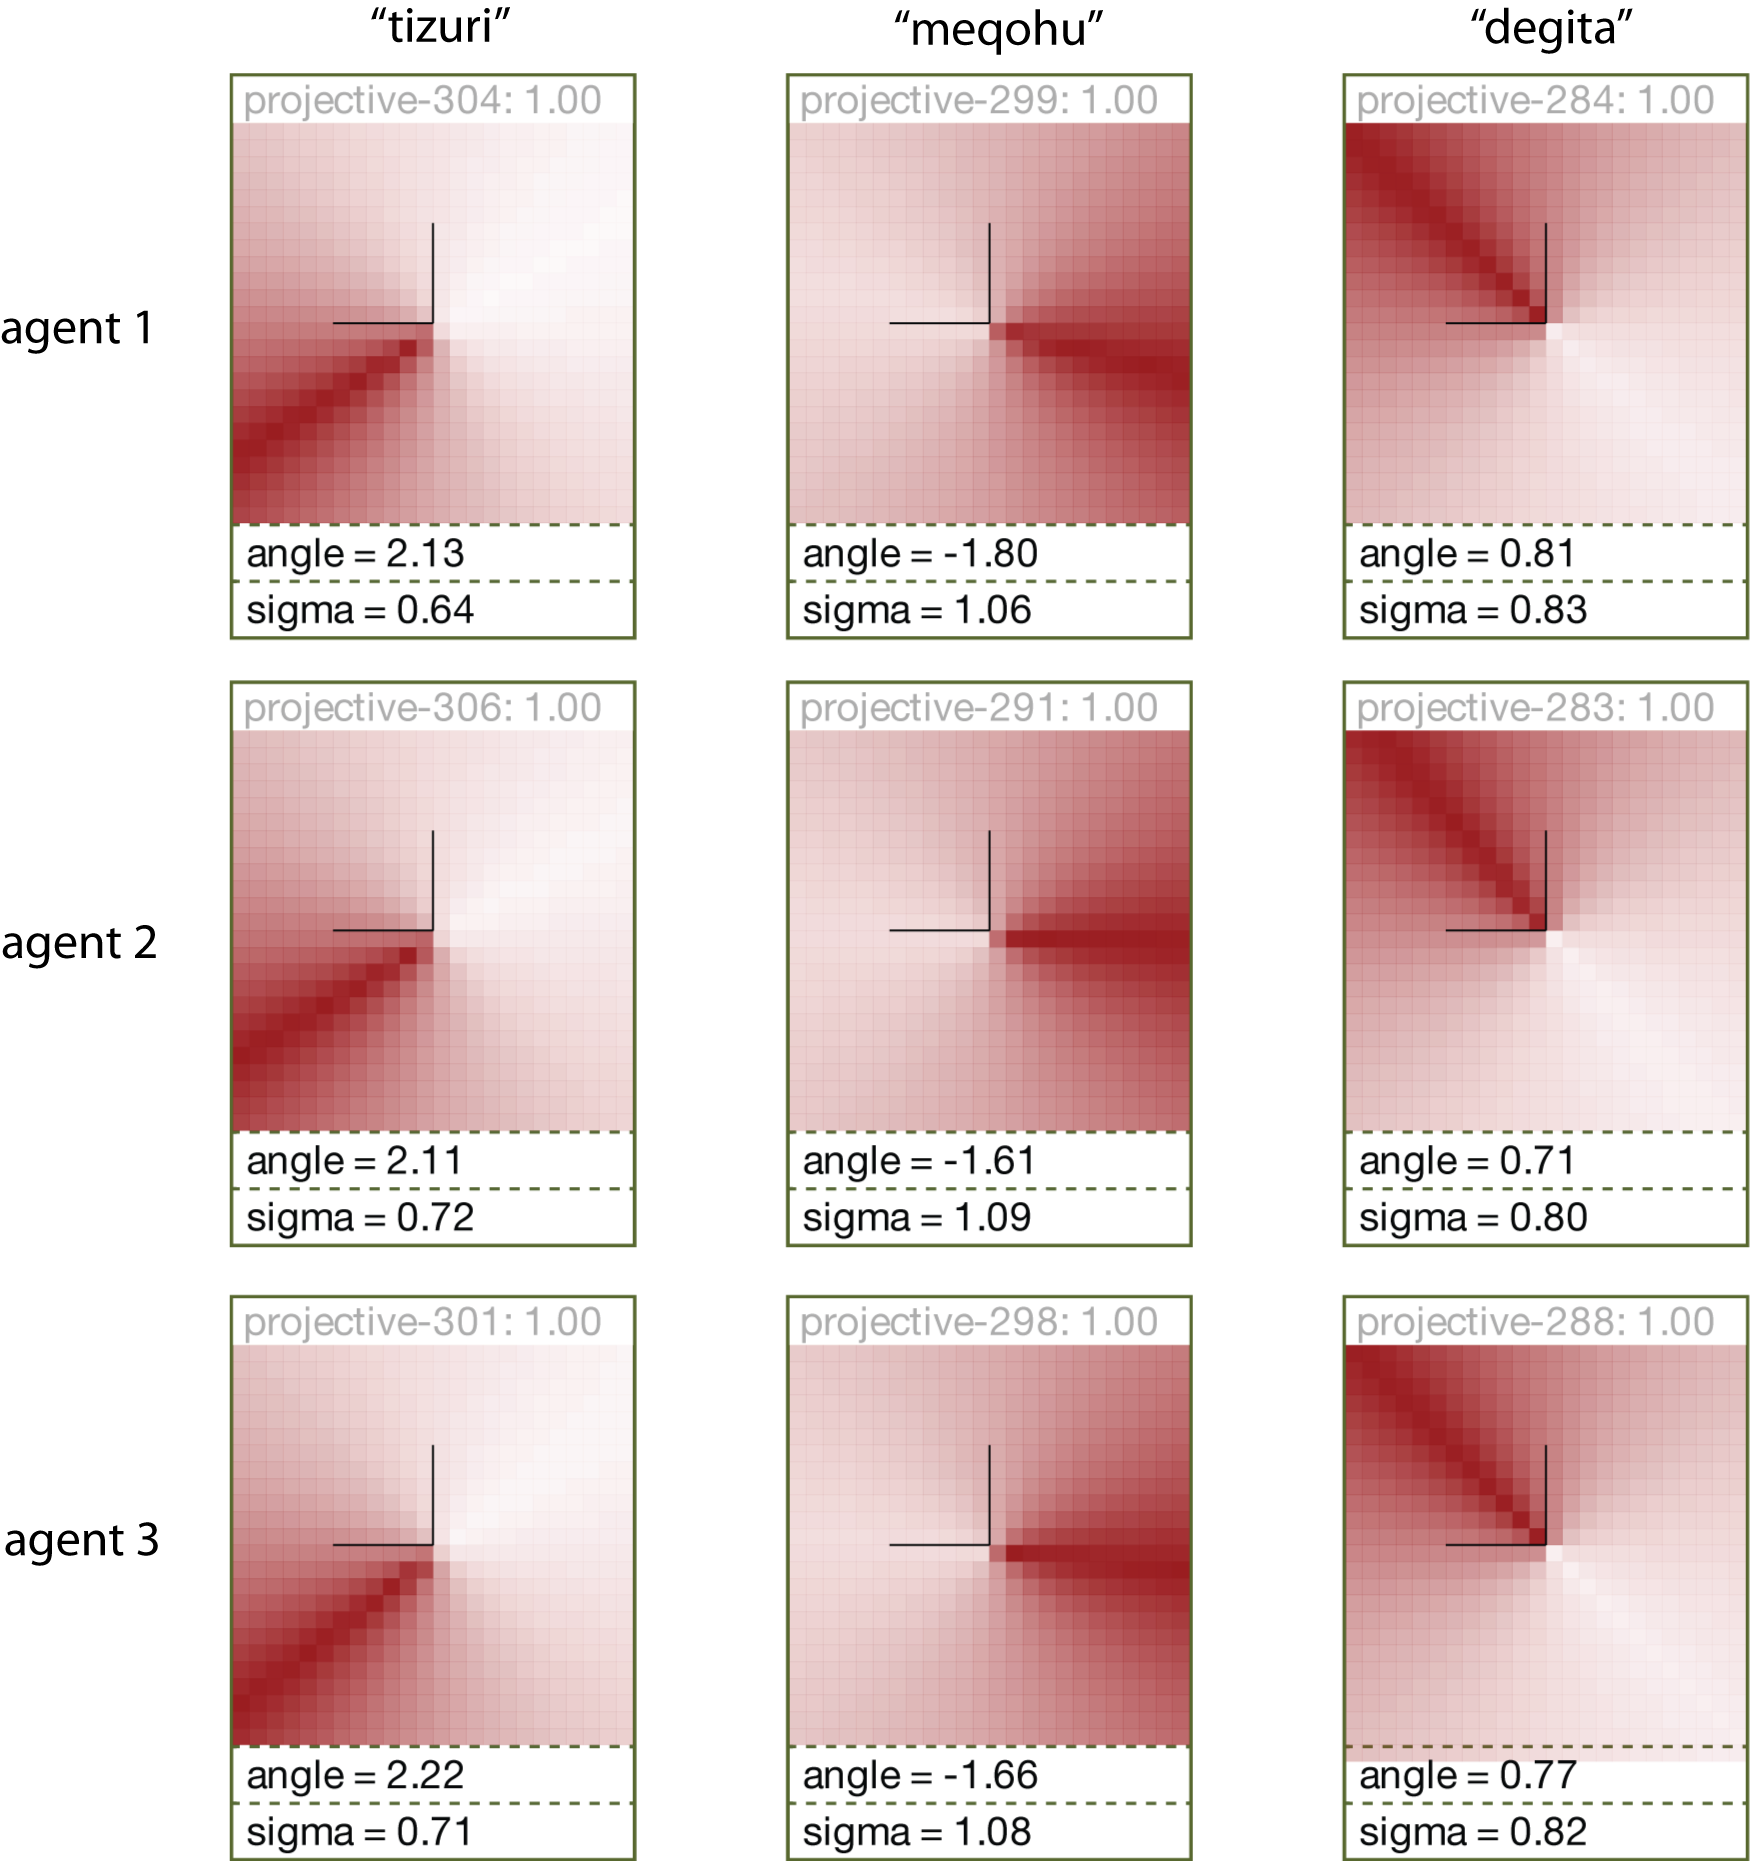
\includegraphics[width=0.75\columnwidth]{figs/category-formation-projective-results+categories-2.png}
\end{center}
\caption[Results formation of projective category systems]{%
Results for a formation experiment in which agents form
a projective category system (top). The bottom figures show the categories and words
in the inventories of the first three agents.}
\label{f:category-formation-projective-results}
\end{figure}

\begin{figure}
\begin{center}
% \includegraphics[width=0.9\columnwidth]{figs/category-formation-proximal-results+categories}
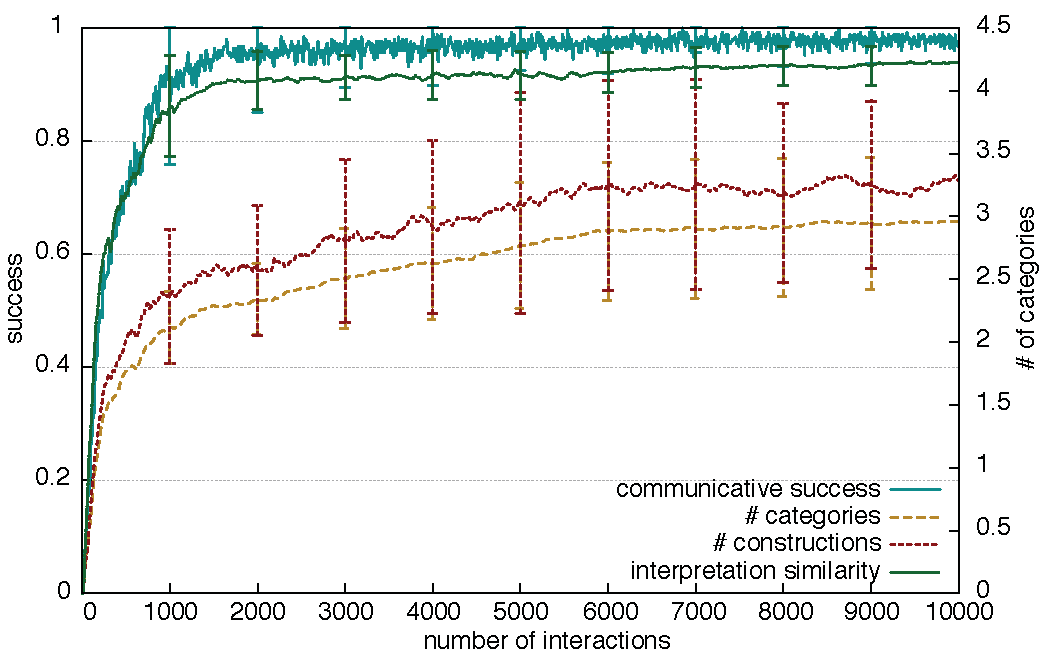
\includegraphics[width=0.8\columnwidth]{figs/category-formation-proximal-results+categories-1}
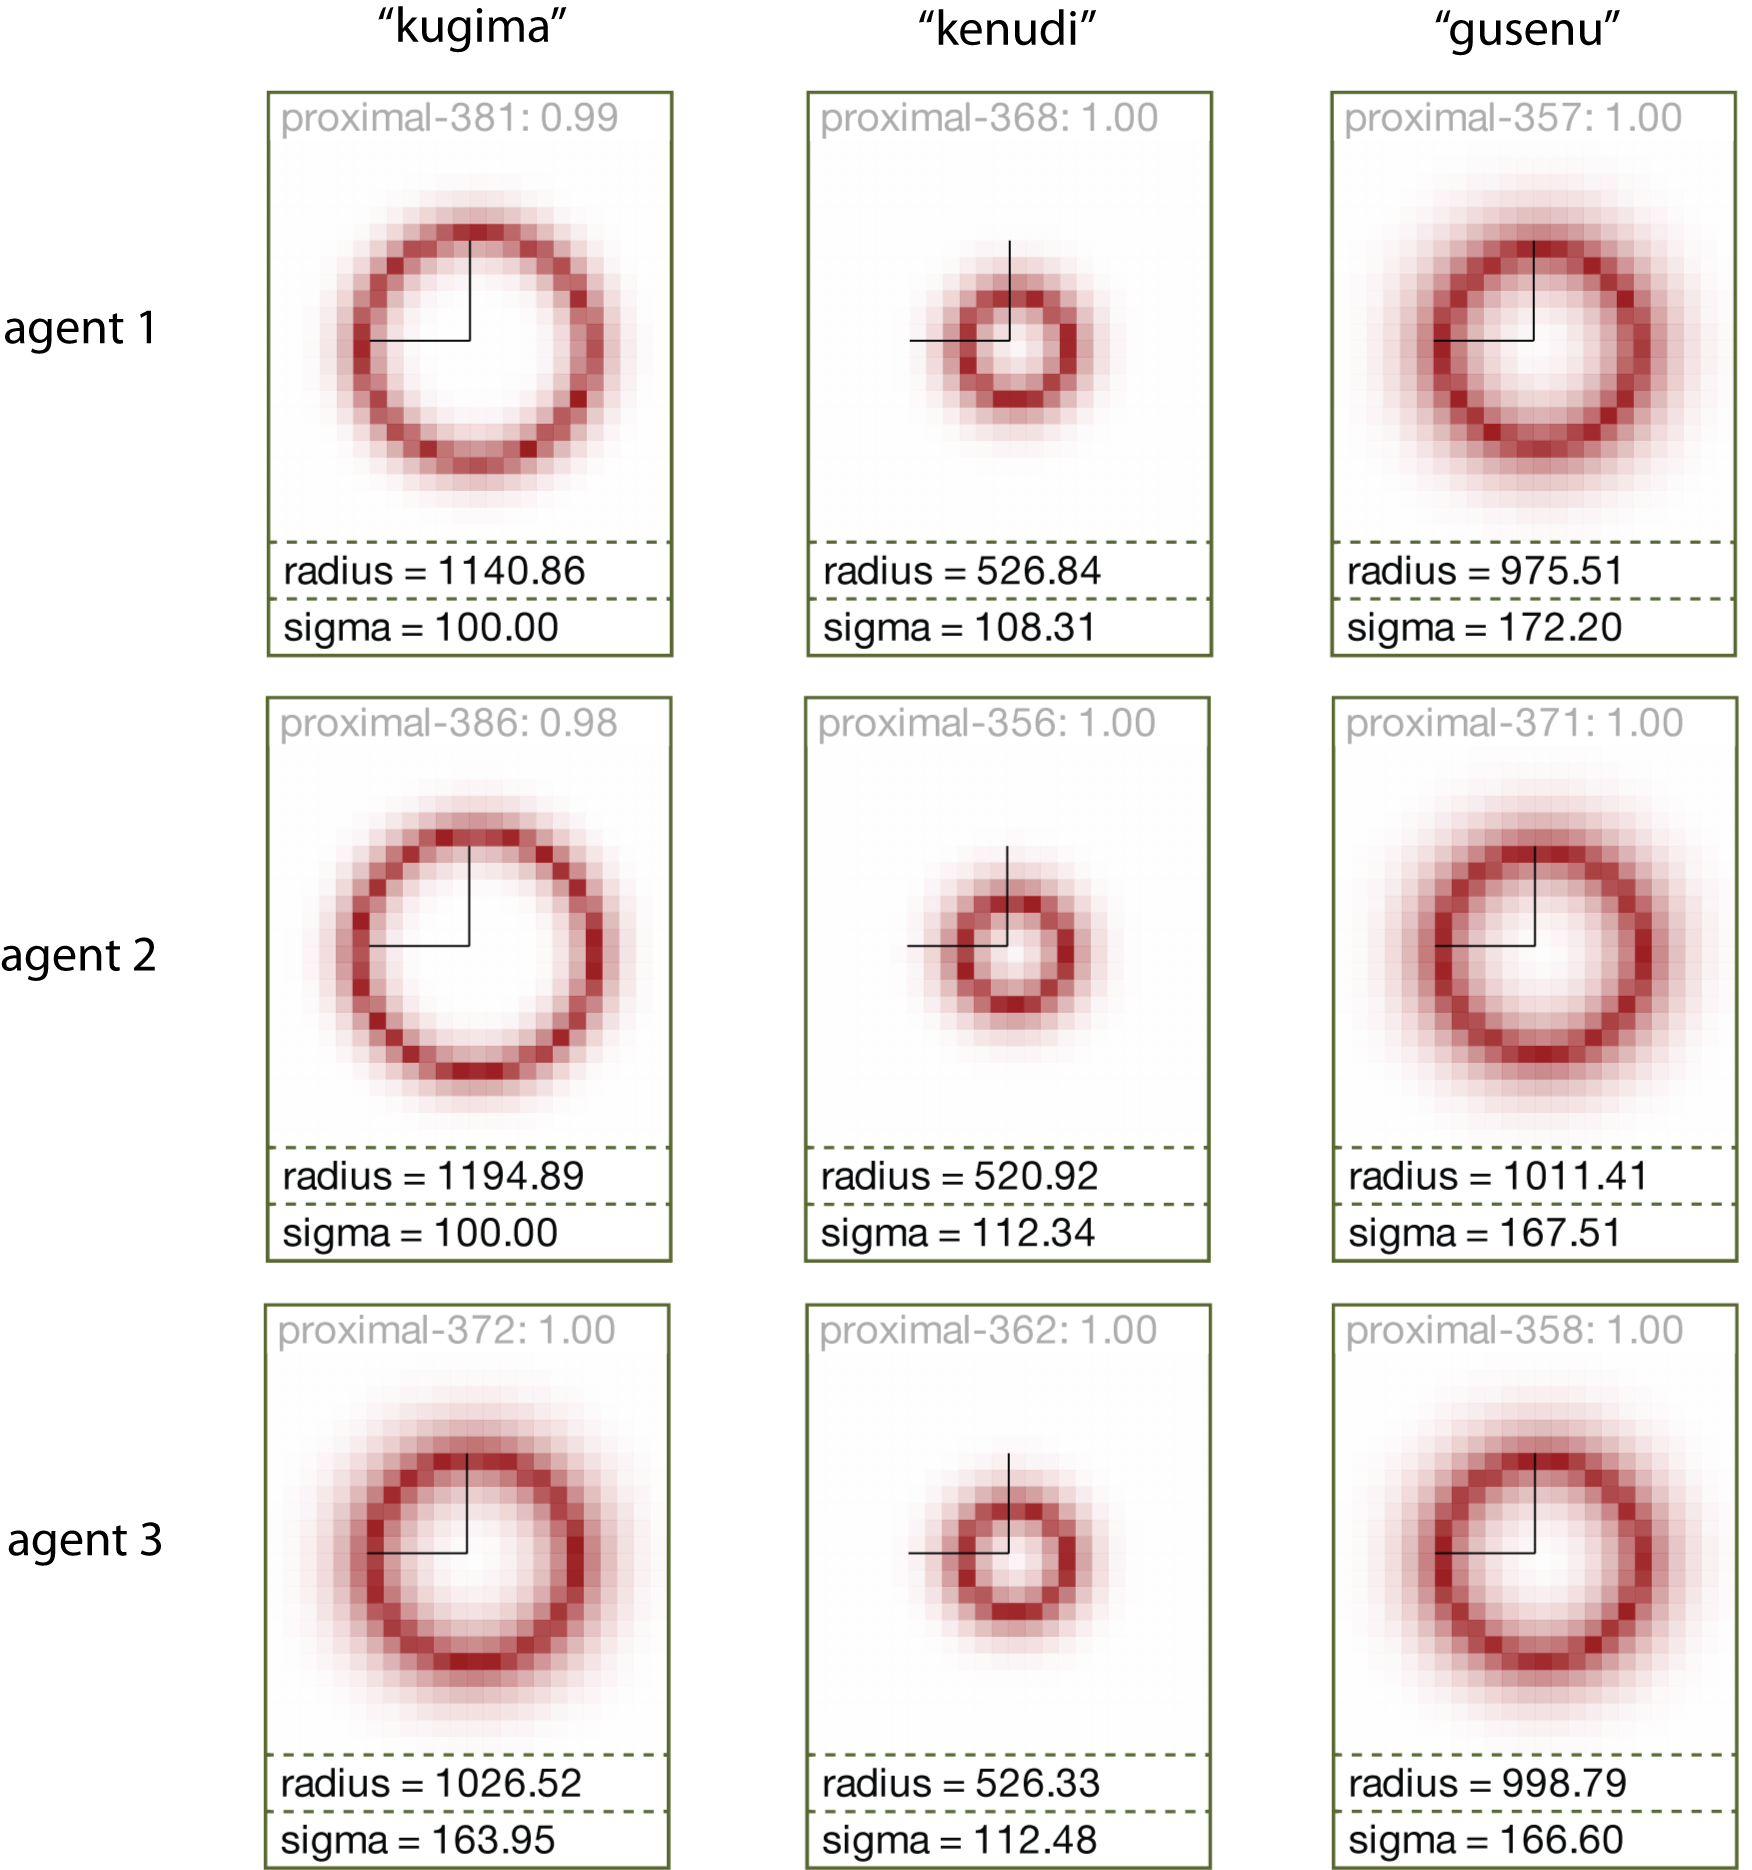
\includegraphics[width=0.8\columnwidth]{figs/category-formation-proximal-results+categories-2.png}
\end{center}
\caption[Results formation of proximal category systems]{Results 
for a formation experiment in which agents form
a proximal category system (top). The bottom figures show the categories and words
in the inventories of the first three agents.}
\label{f:category-formation-proximal-results}
\end{figure}

\begin{figure}
\begin{center}
% \includegraphics[width=0.9\columnwidth]{figs/category-formation-absolute-results+categories}
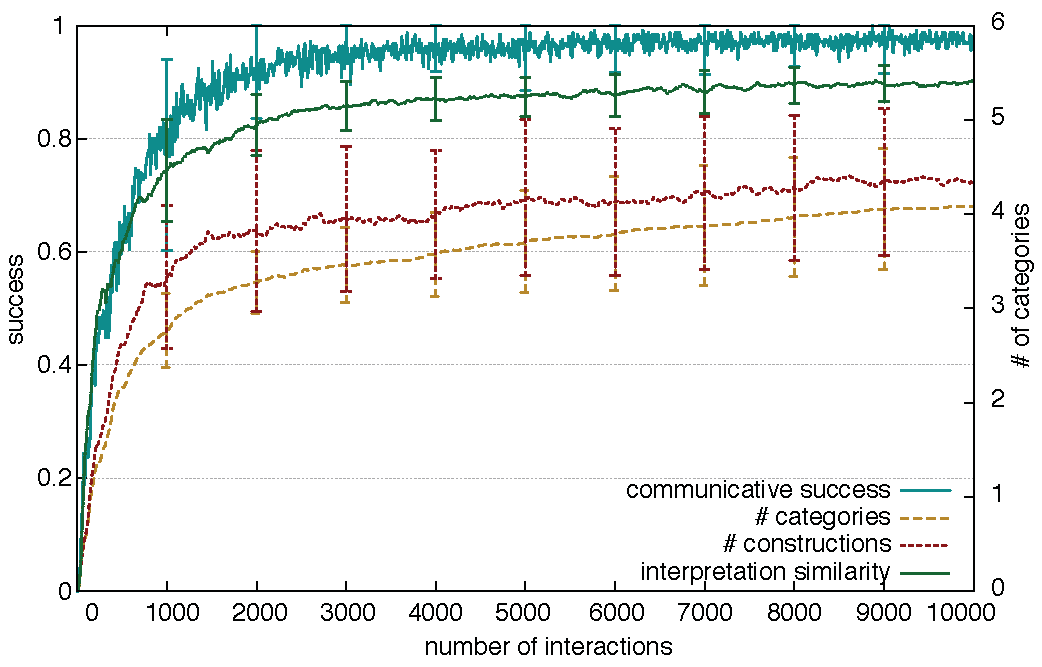
\includegraphics[width=0.85\columnwidth]{figs/category-formation-absolute-results+categories-1}
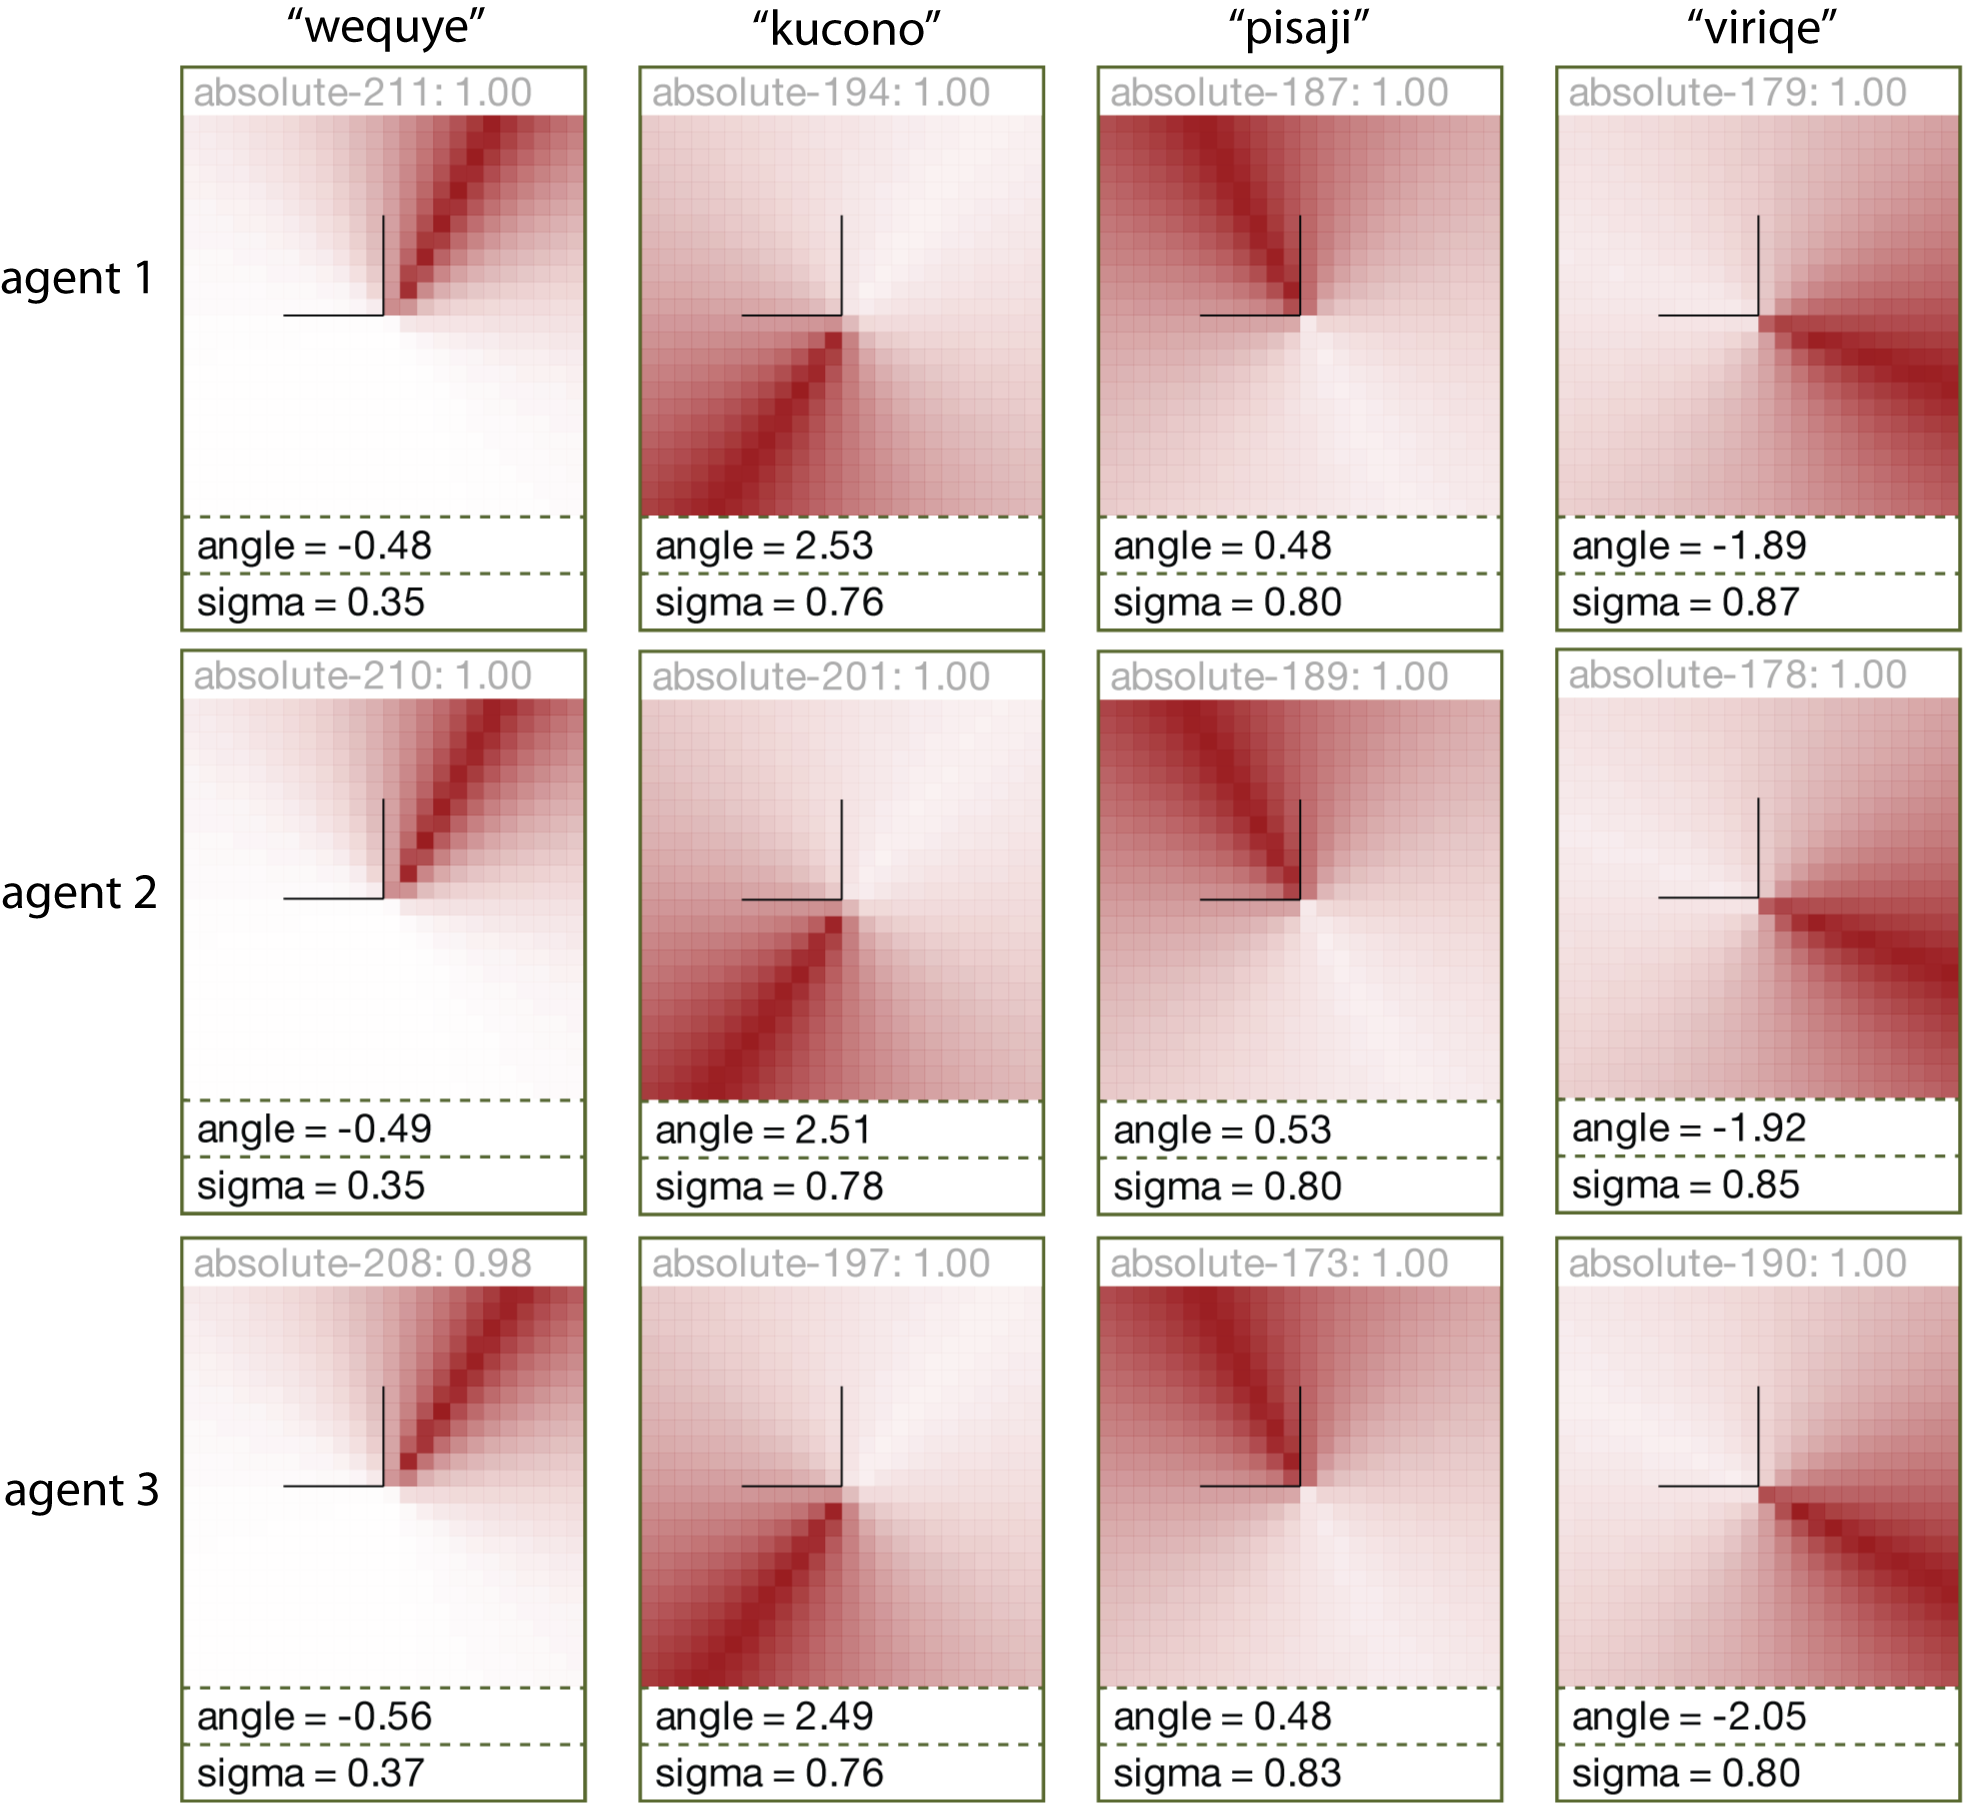
\includegraphics[width=0.85\columnwidth]{figs/category-formation-absolute-results+categories-2.png}
\end{center}
\caption[Results formation of absolute category systems]{Results 
for a formation experiment in which agents form
an absolute category system (top). 
The bottom figures show the categories and words
in the inventories of the first three agents.}
\label{f:category-formation-absolute-results}
\end{figure}

To shed some light on the two factors, I explore how the
system reacts by manipulating each of the two parameters separately. In particular,
one can study the systems emerging when the same strategy is applied in multiple runs
to the same set of contexts, how different strategies perform on the same set of contexts 
and how the same strategy performs when applied to different sets of spatial scenes. 
In Figures \ref{f:category-formation-projective-results} to \ref{f:category-formation-absolute-results} 
experiments are shown in which 25 times the same strategy is used to build either a
projective, a proximal or an absolute language system. Each of these 25 runs across the 
different strategies are performed on the same set of spatial scenes ({\footnotesize\tt space-game-2} 
for the projective language system, {\footnotesize\tt space-game-3} for the proximal system and a
combination of scenes from {\footnotesize\tt space-game-2} and {\footnotesize\tt space-game-9} for the absolute
system).  The only difference between different runs is which particular context was
randomly chosen in each interaction as well as which agents from the population participate
in each interaction. The graphs suggest given the same environmental conditions 
the system settles on the same number of spatial categories in different runs. A fact that is supported by measuring
the similarity of categories across experiments in this case $0.749$. Category similarity of 
populations is computed by maximizing the similarity of each agent of one population to each
agent of the other population and averaging the results. So in that sense $0.749$ is a rather high
number which quantifies the amount of similarity in the category systems of different
populations. We can conclude then that in the same environmental conditions the 
same strategy will develop very similar category distinctions. This, of course, only extends 
to the similarity of the categories themselves. The words floating in each population are different from 
other populations.

\begin{figure}
\begin{center}
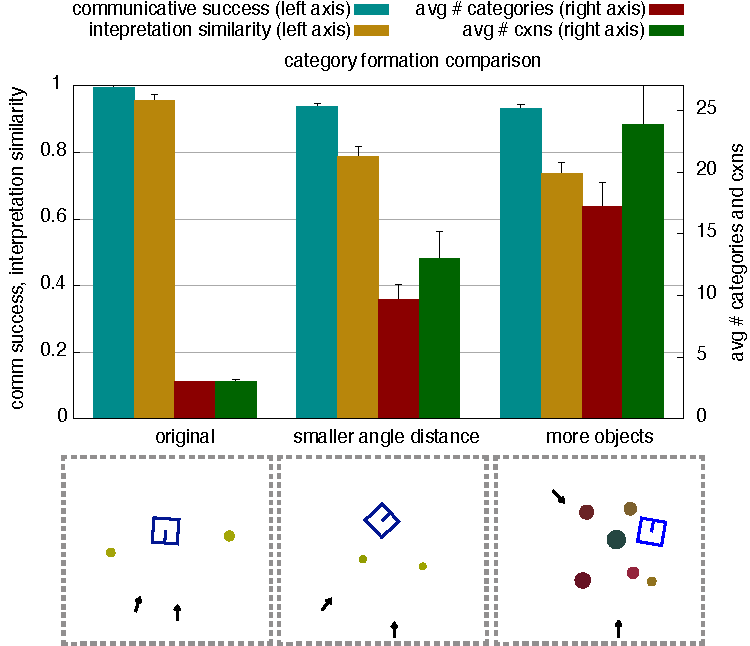
\includegraphics[width=1.0\columnwidth]{figs/category-formation-projective-compare-original-smaller-angle-more-objects}
\end{center}
\caption[Impact of different environmental conditions on 
projective systems]{%
Comparison of the impact of different environmental conditions on the language
system built by the projective language strategy. The {``original''} condition repeats the results 
from Figure \ref{f:category-formation-projective-results}. In the {``smaller angle distance''} condition
agents are facing two objects in each context that have a smaller angle distance than in the
{``original''} condition. The last condition is the {more objects} condition in which each context has 
on average $5.27$ objects. This entails that also the average angle distance is lower than in the original condition 
($1.64$ as opposed to $2.13$). The difference is roughly speaking a semi-circle.
Example scenes for each condition can be seen below.
A clear increase in the number of categories\is{measures!number of categories} for the two conditions {``smaller angle distance''} and 
``more objects'' can be observed (right axis). The graphs are generated by averaging the results 
from 25 runs in each condition of 10000 interactions in which agents form a language system and 10000
interactions where the developed system is just tested without further invention and alignment.}
\label{f:compare-original-smaller-angle-more-objects}
\end{figure}

The second interesting question is: what are the differences in language systems that
the same strategy builds when facing distinctly different environmental conditions? 
Let us look at the projective case. The results in Figure \ref{f:category-formation-projective-results}
were obtained on a set of spatial scenes in which each context consists of two objects
which have a mean angular distance of $2.13$, that is, the two objects in every context
are on average a semicircle apart from each other. I compare the results of
the projective language strategy on this data set to data sets in which the number of 
objects is varied and in which the mean angle distance between two objects is different. 
Figure \ref{f:compare-original-smaller-angle-more-objects}
shows the impact of these two manipulations. From these graphs we can
conclude that less angular distance between objects in spatial scenes require agents 
to make more distinctions which can be seen by the increase in categories 
emerging in the ``smaller angle distance'' condition. However, the real driving force 
behind invention of more distinctions seems to be related to the number of objects per context,
for which the corresponding ``more objects'' condition shows a massive increase in emerging
categories. In all three conditions, nevertheless, the system is able to stabilize on 
high average success proving the successful adaptation of the emerging language
system to different environmental conditions. 

A word of caution is in place here. There is no direct correlation between either number of 
objects nor average angle distance and the number of categories\is{measures!number of categories} needed for discrimination. 
There are always border cases in which, for instance, a small average angle distance still leads to 
few distinctions. Consider environmental conditions in which in every context, two objects are 
at the same position a tiny angle distance
apart from each other. In such a world agents will develop a projective category system
consisting of two categories only, since this is sufficient for discrimination.
In spite of such border cases, the general point is still valid. The less angle distance
and the more objects in each context, the more likely it is that agents need to develop
more category distinctions in order to be successful \emph{and} the systems presented in this
chapter allow agents to invent these necessary distinctions.

Finally, one can study other influences on the dynamics of language evolution
given the operators discussed in this section. One factor of interest is, for instance,
the population size. Figure \ref{f:impact-population-size} shows the impact different
population sizes have on the alignment and evolution of a projective language
system. The figure shows that the systems discussed in this section are
resilient to increases in population sizes and cope well with large populations of at
least up to 100 agents (which is the maximum number of agents tested).

\subsection{Interaction of strategies}
The influence of environmental conditions on the unfolding language system 
can be studied separately with respect to each categorization strategy be
it absolute, projective or proximal, but it can also be examined with respect
to the interaction of these different strategies. In the previous section 
I discussed the simultaneous acquisition of two language systems a projective and
a proximal one via {semantic inference}\is{semantic inference}, a mechanism
that allows agents to decide between different strategies based on discriminative power
(the mechanism is described in Section \ref{s:category-acquisition}). 
I extend this principle to formation of lexical systems by giving agents 
two categorization strategies, e.g., proximal and projective, at the same time 
and also equipping them with two invention strategies. 
Figure \ref{f:category-formation-proximal+projective-results}, for instance, 
shows agents developing proximal and projective categories at the same time. 
For such a coupled system environment factors are again the driving force behind 
the particular language system that is emerging. In environmental conditions where
objects in each context are at large distance from each other, proximal distinctions
should be more important and, thus, develop more strongly than, for instance, 
in environmental conditions where objects are situated with larger angle distance. 
Figure \ref{f:compare-projective+proximal} shows that this is the case.

\subsection{Hybrid systems}
Lastly, one can consider a system were agents do not have different strategies 
focussing on a particular sensory channel, but where they have one strategy 
which allows them to develop the channel focus autonomously. 
This continues the strand of categorization introduced in
Section \ref{s:category-acquisition}. In order, to test this strategy in formation
the system for acquisition is extended by invention operators that allow
speakers to introduce spatial categories and lexical items for expressing them.
Figure \ref{f:proximal-angular+results} shows that this strategy can also be
successfully used to form a language system.

\section{Summary}
This chapter has shown how populations can (a)
acquire, and (b) co-evolve an ontology and lexicon of spatial relations 
provided that they are equipped with a conceptualization strategy 
and invention, adoption and alignment operators. 
Moreover, this chapter studied the interaction of different language strategies
particularly with respect to environmental conditions. We can conclude that
the proposed operators allow agents to acquire and develop successful category systems
under certain conditions. 


\begin{figure}
	\begin{center}
		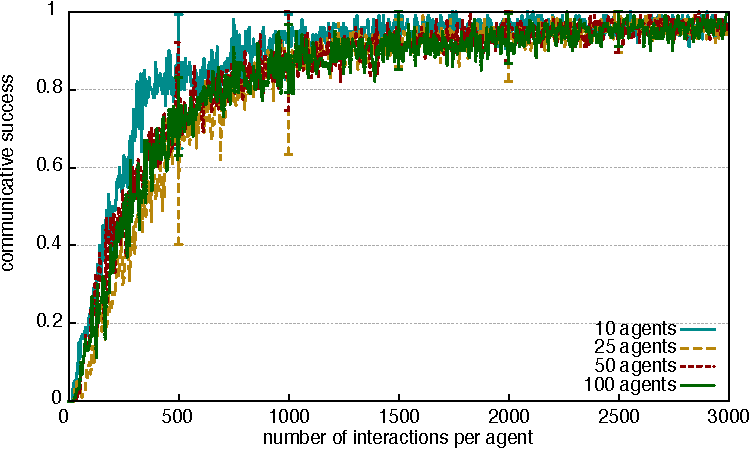
\includegraphics[width=0.9\columnwidth]{figs/category-formation-experiment-success-vs-population-size}
		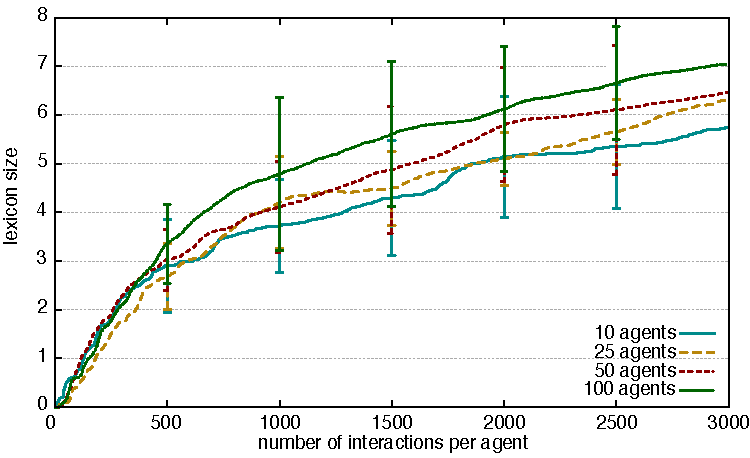
\includegraphics[width=0.9\columnwidth]{figs/category-formation-experiment-lexicon-size-vs-population-size}
	\end{center}
	\caption[Impact of population sizes on category formation]{%
		Impact of population sizes on category formation. On the x-axis is plotted number
		of interactions per agent. This is different from all other graphs discussed in this section.
		The figure shows that population size increases have a negligible effect on the dynamics
		of communicative success\is{measures!communicative success} and the developing ontology of spatial relations.}
	\label{f:impact-population-size}
\end{figure}


\begin{figure}
	\begin{center}
		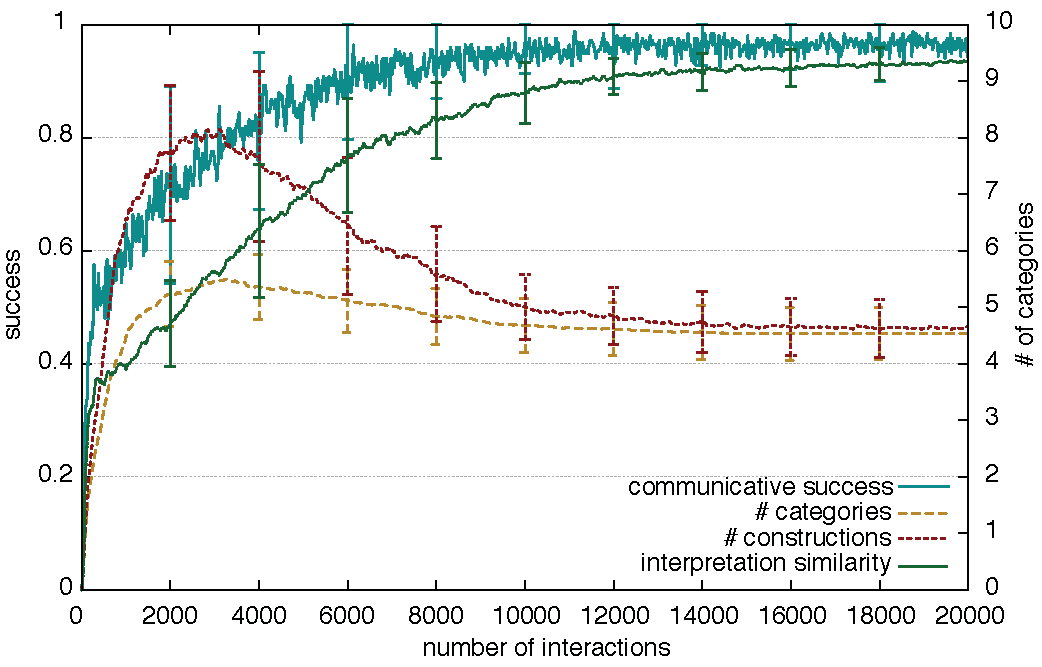
\includegraphics[width=0.8\columnwidth]{figs/category-formation-proximal+projective-results+categories-1}\\
		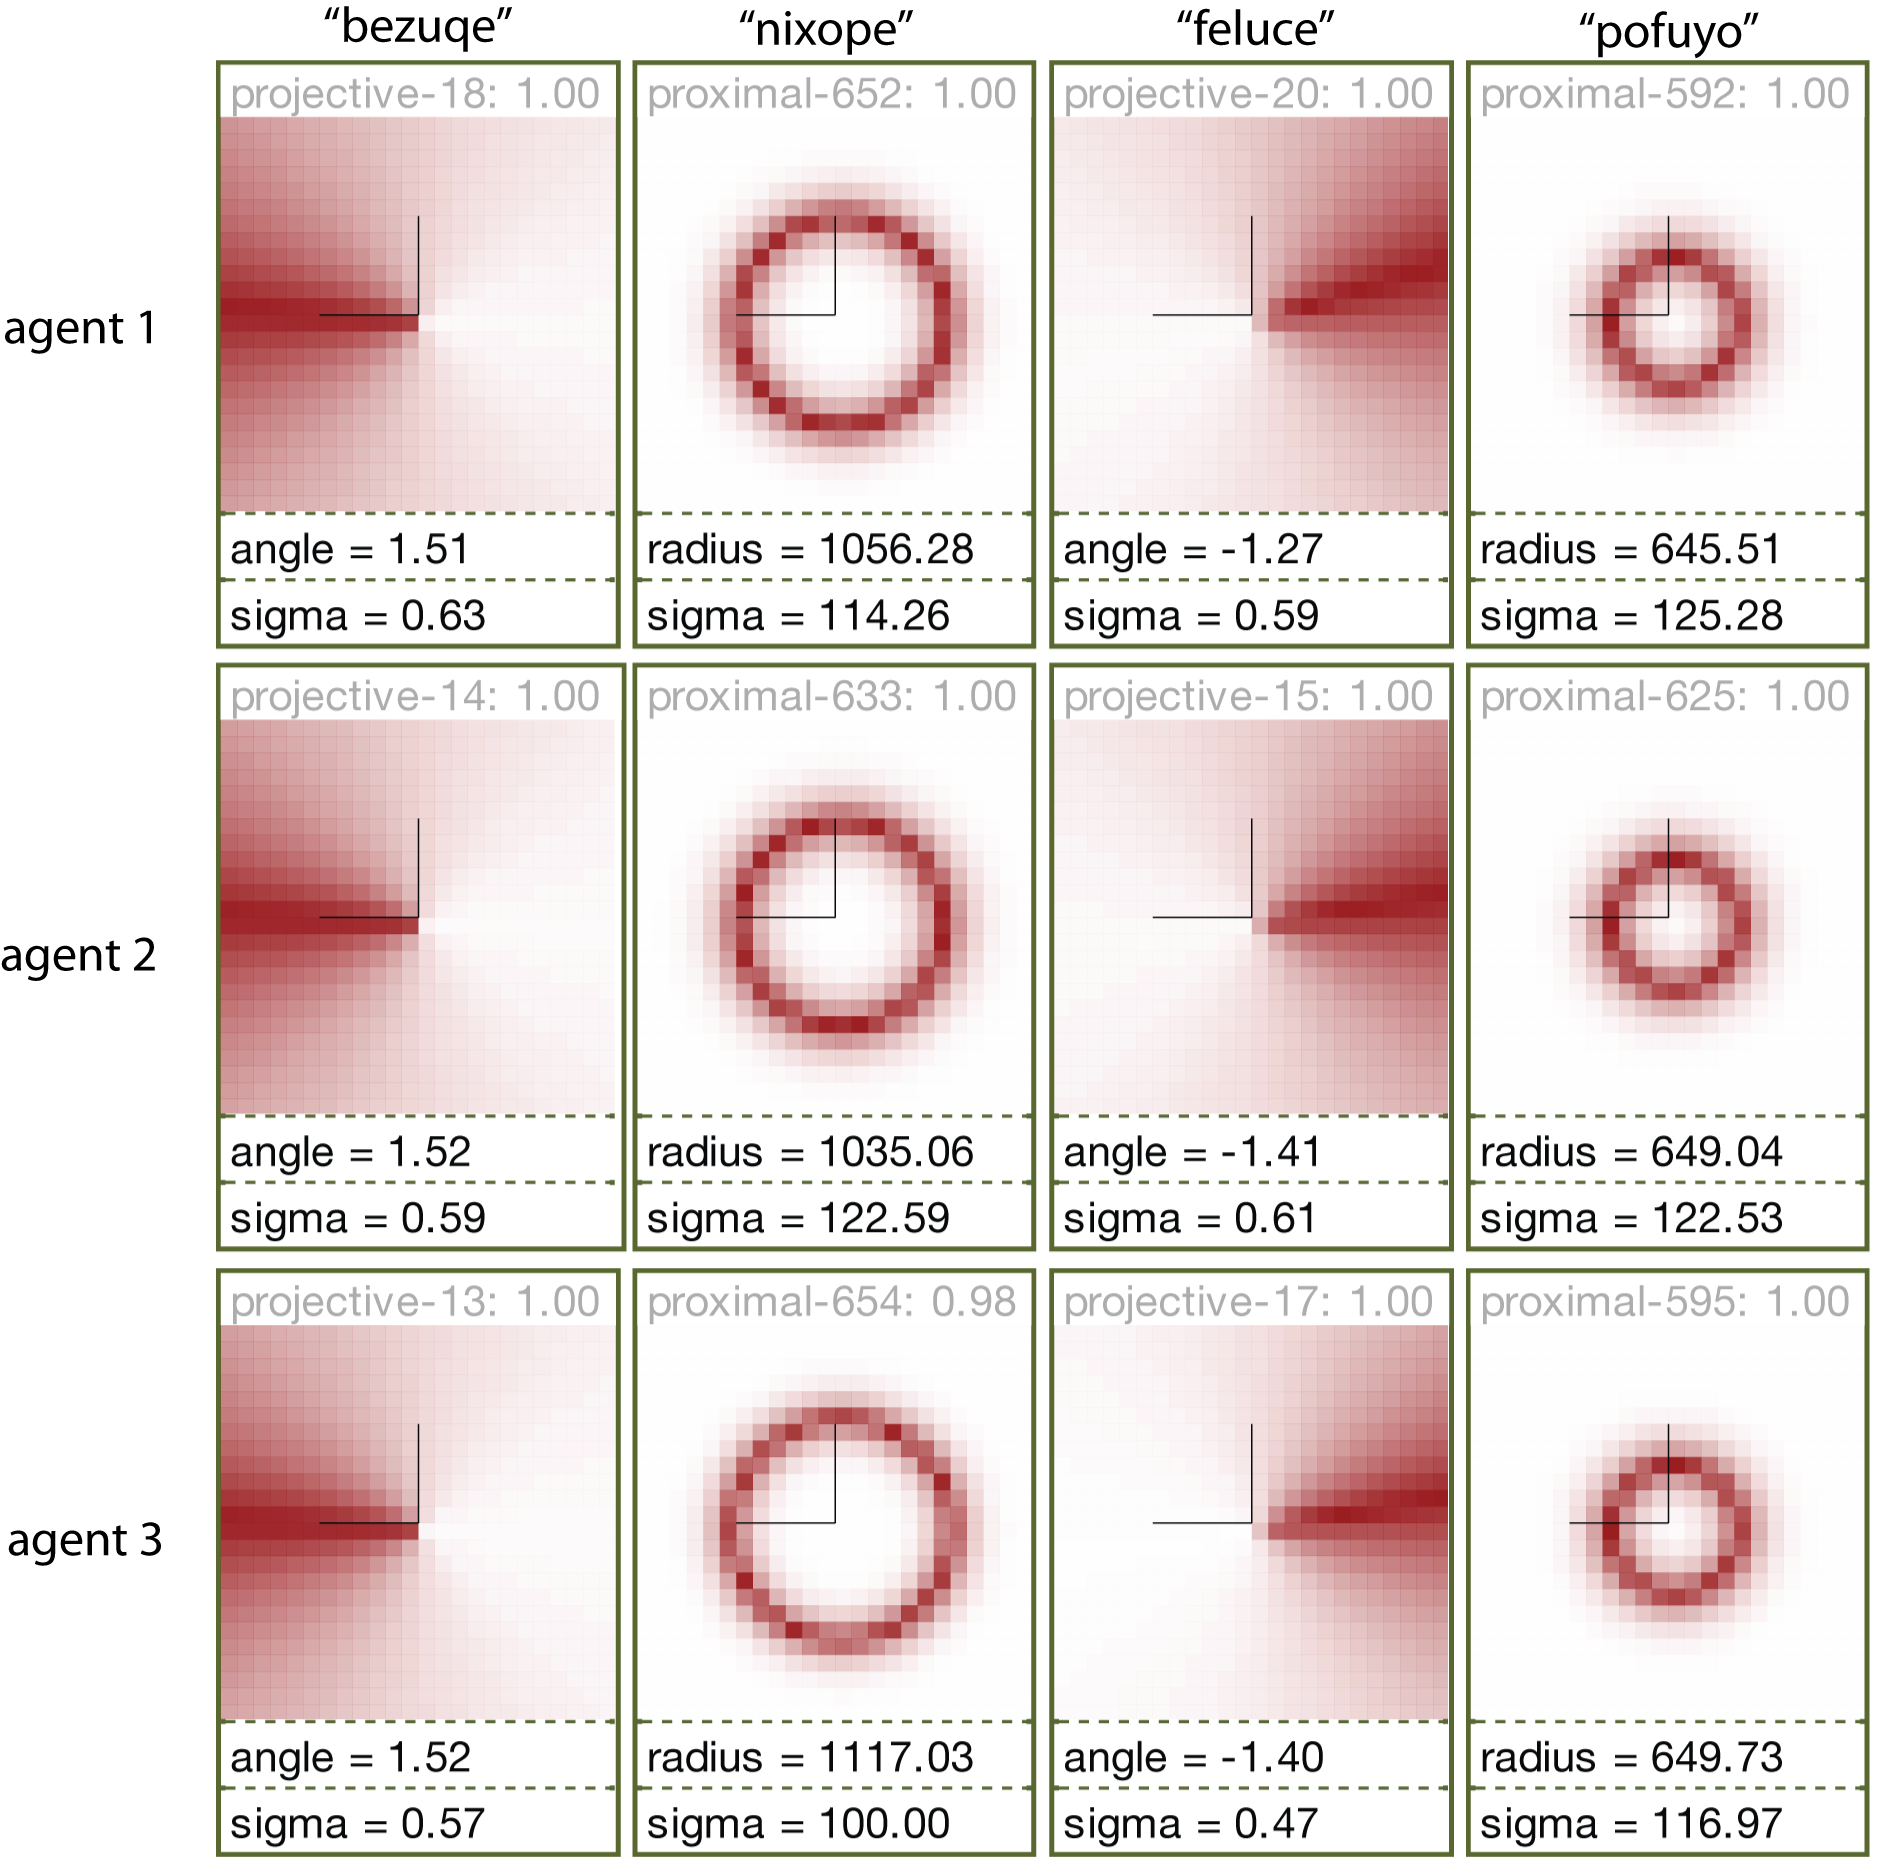
\includegraphics[width=0.8\columnwidth]{figs/category-formation-proximal+projective-results+categories-2.png}
	\end{center}
	\caption[Results simultaneous formation of proximal and projective systems]{Results for a formation experiment in which agents are equipped simultaneously
		with a proximal and projective strategy. In invention, agents use the principle of maximizing discriminative power
		to choose between the two strategies.}
	\label{f:category-formation-proximal+projective-results}
\end{figure}

\begin{figure}
	\begin{center}
		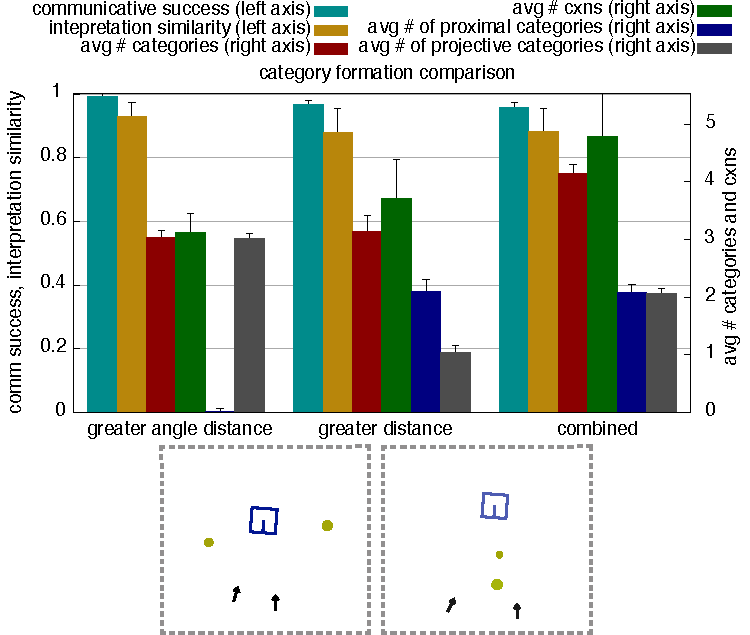
\includegraphics[width=1.0\columnwidth]{figs/category-formation-proximal+projective-compare-angle-distance-distance-combined.pdf}
	\end{center}
	\caption[Impact of different environmental conditions on 
	proximal and projective systems]{Comparison of the impact of 
		different environmental conditions on the language
		system build by a combined projective and proximal language strategy. In environmental
		conditions where objects exhibit large angle distances (bottom left shows an example scene) 
		agents prefer to rely on projective categories that allow to discriminate objects based on angle. 
		In conditions where there is a bigger distance between objects (bottom right image) 
		than angle distance agents chiefly rely on
		proximal categories. In the ``combined'' condition which has both scenes with 
		large angle distance as well as scenes with large distances between objects a balanced
		language system consisting of proximal and projective categories is developed.}
	\label{f:compare-projective+proximal}
\end{figure}

\begin{figure}
\begin{center}
% \includegraphics[width=1.0\columnwidth]{figs/category-formation-proximal-angular-results+categories}
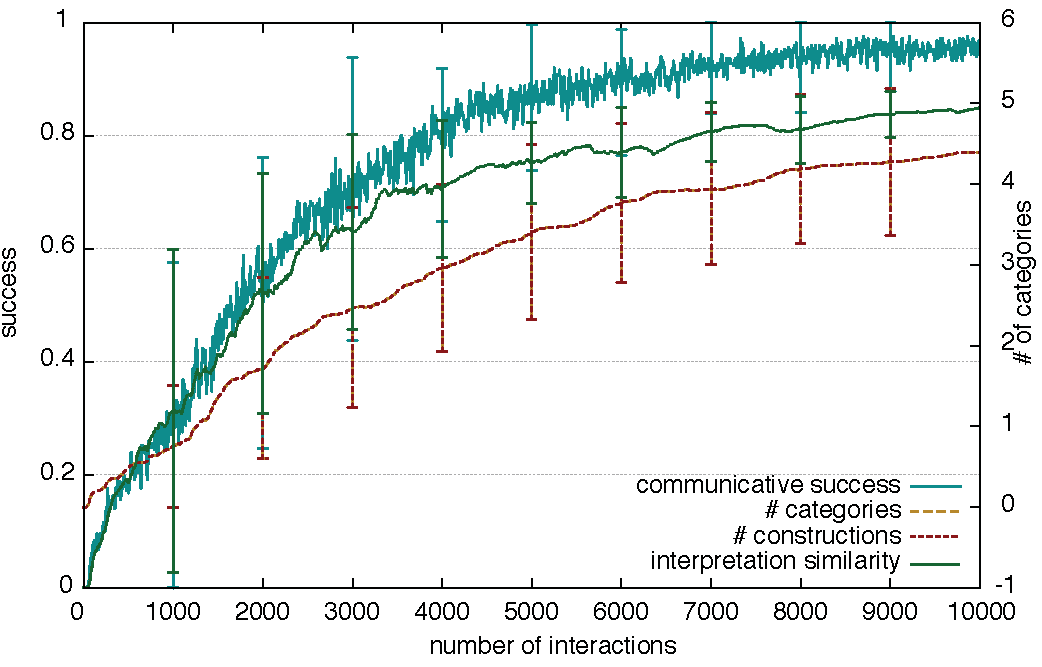
\includegraphics[width=0.9\columnwidth]{figs/category-formation-proximal-angular-results+categories-1}
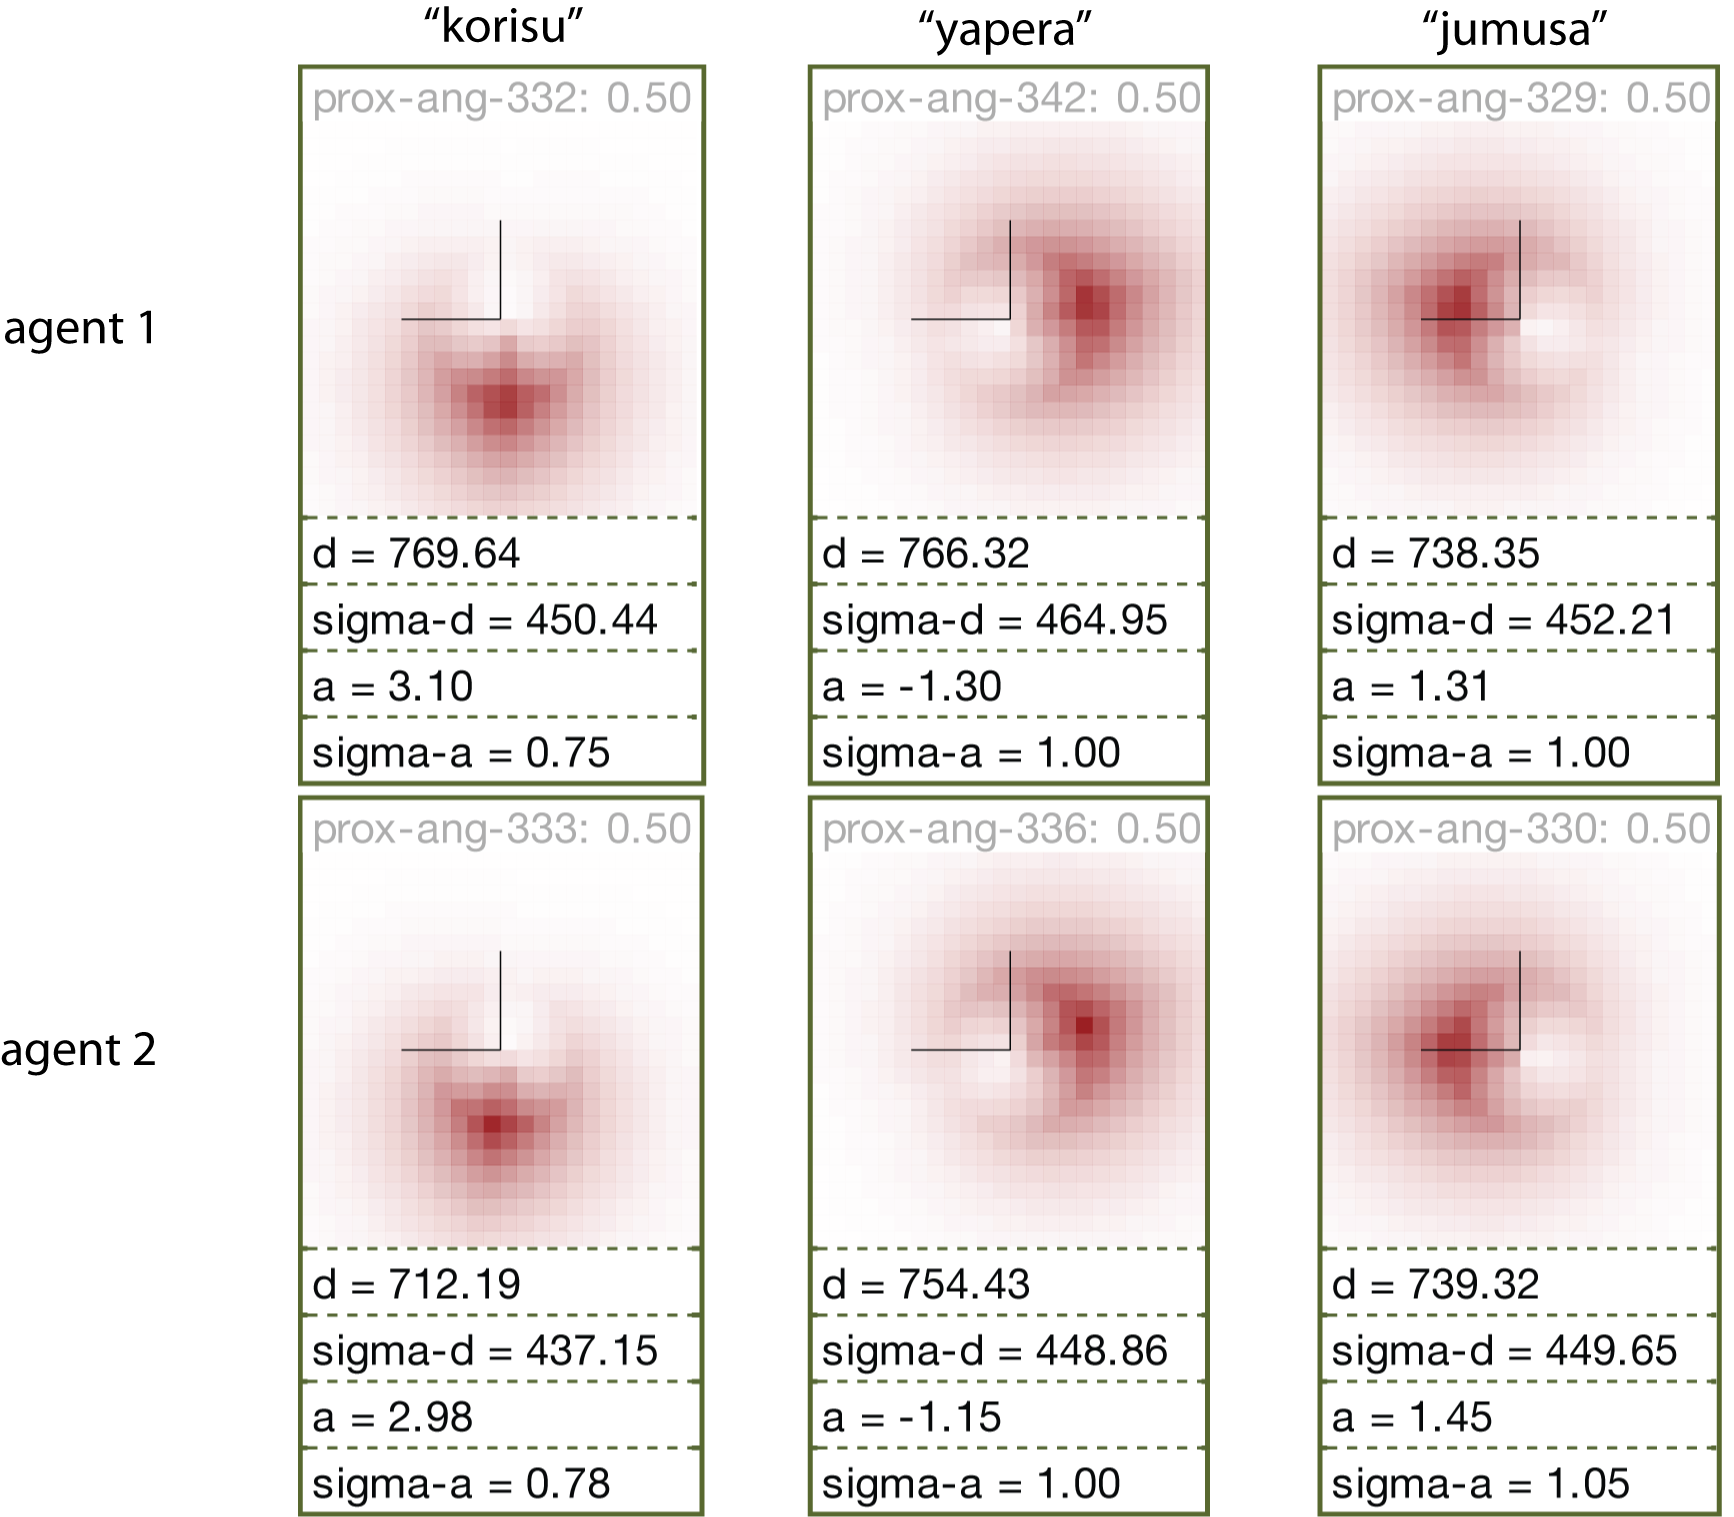
\includegraphics[width=0.8\columnwidth]{figs/category-formation-proximal-angular-results+categories-2.png}
\end{center}
\caption[Results formation of hybrid systems]{Results for a formation 
experiment in which agents are equipped with a hybrid
strategy that does not distinguish between angle and distance 
channel but combines both channels in a single 
category representation.}
\label{f:proximal-angular+results}
\end{figure}



%\bibliographystyle{diss}
%\bibliography{papers,space}
%\end{document}